\part{消化系统疾病急诊}

\chapter{急 性 胃 炎}

胃炎(gastritis)是指各种病因所致胃黏膜炎性病变,是最常见的消化道疾病之一。1990年提出的悉尼胃炎分类法,将胃炎确定为三种基本诊断:急性胃炎、慢性胃炎、特殊类型的胃炎,加上病因学、形态学、部位及内镜诊断。诊断胃炎主要依靠胃镜和组织学检查。

急性胃炎(acute
gastritis)是由各种病因引起的胃黏膜急性炎症,临床上常急性起病,有明显上腹部症状,恶心、呕吐、腹痛、嗳气等;内镜检查可见胃黏膜充血、水肿、出血、糜烂(可伴有浅表溃疡)等一过性病变;病理组织学特征为胃黏膜固有层见到以中性粒细胞为主的炎症细胞浸润。它可以不仅局限于胃,同时伴随食管炎症者称食管胃炎,伴随肠道炎症者称胃肠炎。根据其病因不同,临床上一般可分为以下几种类型:①急性幽门螺杆菌感染引起的急性胃炎:健康志愿者吞服幽门螺杆菌后的临床表现、内镜所见及胃黏膜活检病理组织学均显示急性胃炎特征。但临床上很难诊断幽门螺杆菌感染引起的急性胃炎,因为一过性的上腹部症状多不为患者注意,亦极少需要胃镜检查,加之可能多数患者症状很轻或无症状。感染幽门螺杆菌后,如不予治疗,幽门螺杆菌感染可长期存在并发展为慢性胃炎。②急性糜烂出血性胃炎(acute
erosivehemorrhagic
gastritis):又称急性胃黏膜病变(AGML),其特点是胃黏膜急性多发性糜烂和出血,或伴有浅表性溃疡,诱因有严重感染、颅脑损伤、严重烧伤、休克等。③急性腐蚀性胃炎(acute
corrosive
gastritis):系由于吞服强酸、强碱或其他腐蚀剂所造成的胃黏膜损伤,主要的病理变化为黏膜充血、水肿和黏液增多,严重者可发生糜烂、溃疡、坏死、甚至穿孔。④急性单纯性胃炎(acute
simple
gastritis):又称急性非特异性胃炎、急性浅表性胃炎,是由各种化学因素(如药物、酒精、浓茶、咖啡和香料等)、物理因素(如进食过冷过热、粗糙食物等)、微生物感染或细菌毒素等外源性刺激因子以及精神神经功能障碍、应激、变态反应等内源性刺激因子,引起的胃黏膜急性炎症。最常见,本章以其为代表。

\subsection{病因与发病机制}

急性胃炎的病因颇多,大致可分为内源性和外源性两类。有害物质通过血流或通过神经体液调节障碍引起胃黏膜急性炎症者,称内源性病因;通过口腔进入胃内引起胃黏膜急性炎症者,称外源性病因。

常见的内源性病因有病毒和细菌感染性疾病,如白喉、猩红热、肺炎、伤寒、肝炎、流感等。其他严重的全身性疾病,如尿毒症、肝硬化、慢性肺心病呼吸衰竭,以及精神神经功能障碍,应激状态或各种因素所致的机体变态反应均属内源性病因范畴。外源性病因有化学性(药物)、物理性(温度的和机械的)因素、微生物感染或细菌毒素。化学刺激可来自烟草(烟草中含有尼古丁等物质)、烈酒、浓茶、咖啡、香料和调味品,内服药物如水杨酸盐类和吲哚美辛等解热镇痛药、磺胺、肾上腺皮质激素、呋喃唑酮(痢特灵)、呋喃妥因(呋喃坦丁)、某些抗生素、抗肿瘤药物、洋地黄、氯化钾、氨茶碱、铁剂等均可刺激胃黏膜;物理刺激如过烫、过冷、过于粗糙的食物;进食被细菌或其毒素污染的食物,可引起急性胃肠炎,致病细菌以幽门螺杆菌、沙门菌属及副溶血弧菌(嗜盐菌)为常见,毒素以金黄色葡萄球菌毒素为常见,而以肉毒杆菌毒素所引起的病情最为严重。病毒感染常为流感、肠道病毒等。

急性胃炎的发病机制主要由于致病因子损伤了胃黏膜防御机制。后者包括黏膜屏障、黏液HCO\textsubscript{3}
\textsuperscript{−}
屏障、上皮快速修复功能、黏膜血流、前列腺素以及某些调节肽(表皮生长因子、生长抑素等)。各成分相互联系,可防御各种外来、内在的损害因子的损伤。而胃炎的发生首先是由于各种过强的损害因子直接或间接削弱胃黏膜防御机制的某一种或几种成分,胃腔中的H\textsuperscript{+}
反弥散到胃壁,引起血管充血、出血、黏膜水肿等炎症反应,并使胃黏膜受到胃酸、胃蛋白酶的消化而出现糜烂、出血。NSAIDs抑制环氧合酶(CoX-1)活性,抑制前列腺素合成,进而胃黏膜修复功能降低。应激性损伤表现有皮质-腺垂体-肾上腺皮质轴活动亢进。

急性胃炎在病因祛除后,可望在短时间内恢复正常,如病因长期持续存在,可能转为慢性胃炎。

\subsection{诊断}

\subsubsection{病史}

有进食化学药品、某些药物、酒类、饮食不当、暴饮暴食或进食有细菌污染之食物等病史。

\subsubsection{临床表现特点}

急性胃炎的临床表现常因病因不同而异:由于酗酒、刺激性食物和药物引起者,多有上腹部不适、疼痛、纳差、恶心、呕吐等,一般不很严重。食物中毒所致的急性胃肠炎的症状轻重不一,一般在食后数小时至24小时内发病,大多有中上腹部不适、疼痛,甚至剧烈腹绞痛、纳差、恶心、呕吐等,伴有急性水样腹泻,严重者可有发热、失水、酸中毒、休克等中毒症状。体检可有中上腹部及脐周轻压痛,肠鸣音亢进。一般病程短暂,1~2天后即好转自愈。由解热镇痛药如阿司匹林、吲哚美辛、肾上腺皮质激素和应激状态等引起的急性胃炎常以上消化道出血为主要表现。患者多有呕血与黑便,出血也呈间歇发作,大量出血者可发生休克。半数以上患者有上腹部不适、疼痛、纳差、头昏、软弱等症状。病因去除后,短期内可以痊愈。

实验室检查外周血象部分患者白细胞数增多,内镜检查见胃黏膜充血、水肿、片状渗出,并有点状、片状出血。X线钡剂检查则显示胃黏膜水肿、局部激惹。

\subsubsection{诊断注意事项}

以上腹痛为主要症状的急性胃炎应与消化性溃疡、急性胰腺炎、急性胆囊炎和急性阑尾炎等急腹症相鉴别。急性心肌梗死患者可因神经反射表现为上腹痛和呕吐,酷似急性胃炎,故对可疑者应及时作心电图检查。

\subsection{治疗}

\subsubsection{一般治疗}

去除病因,卧床休息,停止一切对胃有刺激性的饮食或药物,进清淡流质饮食,必要时禁食1~2餐。

\subsubsection{对症治疗}

上腹痛较剧烈者肌注阿托品(0.5mg)或山莨菪碱(10mg);或口服颠茄片(8mg,每天3次),或丙胺太林(普鲁本辛)(15mg,每天3次)。伴有呕吐者,可口服甲氧氯普胺(灭吐灵)(10mg,每天3次)或多潘立酮(吗丁林)(10mg,每天3次)或西沙必利(5~10mg,每天2~3次)。亦可针刺足三里和内关,有止痛或止吐效果。伴有腹泻者,可口服双八面体蒙脱石(思密达)(3g,每天3次),或复方地芬诺酯(复方苯乙哌啶片)(1~2片,每天2~4次),或洛哌丁胺(易蒙停胶囊)(2~4mg,每天2~4次)等止泻药物。并发上消化道出血时应予静脉输液,应用H\textsubscript{2}
受体阻滞剂(如雷尼替丁、法莫替丁)或质子泵抑制剂(如奥美拉唑)等药物(详见第13章第1节“上消化道出血”)。

\subsubsection{抗生素的应用}

由细菌感染引起者,可口服诺氟沙星(norfloxacin,氟哌酸)(0.2g,每天3次),或盐酸小檗碱(0.3g,每天3次)等药物,伴腹泻的严重病例可加用庆大霉素或妥布霉素8万U肌注,每天2次;或20万~24万U/d加入液体中静滴。

\subsubsection{维持水电解质平衡}

因呕吐、腹泻导致失水及电解质失衡,可静脉补液,用生理盐水或平衡盐液与5\%葡萄糖液按2∶1或3∶1的比例配合静滴。排尿后适当补钾。酸中毒者可滴注5\%碳酸氢钠。\protect\hypertarget{text00317.html}{}{}

\hypertarget{text00317.htmlux5cux23CHP11-1-4}{}
参 考 文 献

1. 李兆申.现代消化病药物治疗学.北京:人民军医出版社,2005:273

2. 陈灏珠 ,林果为.实用内科学.第13版.北京:人民卫生出版社,2009:1974

\protect\hypertarget{text00318.html}{}{}

\chapter{消化性溃疡}

消化性溃疡(peptic
ulcer,PU)指胃肠道黏膜被胃酸和胃蛋白酶消化而发生的溃疡,好发于胃和十二指肠,也可发生在食管下段、小肠、胃肠吻合口,以及异位的胃黏膜,如位于肠道的Meckel憩室。胃溃疡(gastric
ulcer,GU)和十二指肠溃疡(duodenal
ulcer,DU)是最常见的PU。溃疡的黏膜缺损超过黏膜肌层,不同于糜烂。溃疡一般为单个,胃或十二指肠同时有两个或两个以上溃疡称多发性溃疡;胃和十二指肠均有溃疡称复合性溃疡;溃疡直径大于2.0cm者称巨大溃疡;溃疡深达浆膜层与周围组织粘连,或穿入邻近组织形成包裹性穿孔者称穿透性溃疡。本病多见于男性,发病年龄DU平均为30岁,GU平均为40岁。临床主要表现为慢性、周期性发作的节律性上腹疼痛,可并发出血、穿孔或幽门梗阻,约1\%的GU发生癌变。幽门螺杆菌(helicobacter
pylori,Hp)感染和使用非甾体抗炎药(non-steroidal anti-inflammatory
drug,NSAID)是引起PU发病的两个独立因素。

\subsection{病因与发病机制}

PU的病因与发病机制尚未完全阐明。1910年Schwartz首先提出“无酸,无溃疡”的概念,这是PU病因认识的起点。1983年Marshall和Warren从人体胃黏膜活检标本中找到幽门螺杆菌,随后众多研究认为Hp与PU有密切关系。胃肠黏膜防御作用的削弱以及药物、神经精神等因素与PU发病也有密切关系。目前认为,PU的发生是一种或多种有害因素对黏膜破坏超过黏膜抵御损伤和自身修复的能力所引起的综合结果,而Hp和NSAID是损害胃肠黏膜屏障从而导致PU发病的最常见病因。

\paragraph{幽门螺杆菌}

PU患者Hp感染率高,DU患者中的检出率高达95\%~100\%,GU为70\%以上。前瞻性调查显示Hp感染者溃疡发生率约13\%~23\%,显著高于不伴Hp感染者。用抑酸治疗愈合的溃疡,停药后1年复发率为50\%~90\%,根除Hp治疗后溃疡复发率降低至1\%~5\%,并减少溃疡并发症的发生率。应用根除Hp治疗方案1~2周,不再给予抑酸治疗,4周后复查,溃疡愈合率高于常规抑酸治疗4周的愈合率。部分难治性溃疡在根除Hp后能得到愈合。表明根除Hp可有效治愈溃疡,缩短溃疡愈合时间。至于何以在感染Hp的人群中仅有小部分人发生PU,一般认为这是Hp、宿主和环境因素三者相互作用的不同结果。

Hp感染导致PU发病的确切机制尚未阐明。Hp感染导致DU发病主要有Hp-胃泌素-胃酸学说和十二指肠胃上皮化生学说,该两种学说认为,胆酸对Hp生长具有强烈的抑制作用,正常情况下Hp无法在十二指肠生存,十二指肠球部酸负荷增加是DU发病的重要环节,因为酸可使结合胆酸沉淀,从而有利于Hp在十二指肠球部生长。Hp只能在胃上皮组织定植,因此在十二指肠球部存活的Hp只有当十二指肠球部发生胃上皮化生才能定植下来,而十二指肠球部的胃上皮化生是十二指肠对酸负荷的一种代偿反应。而十二指肠球部酸负荷增加的原因,一方面与Hp感染引起慢性胃窦炎有关,Hp感染直接或间接作用于胃窦D、G细胞,削弱了胃酸分泌的负反馈调节,从而导致餐后胃泌素-胃酸分泌增加;另一方面,吸烟、应激和遗传等因素均与胃酸分泌增加有关。定植在十二指肠球部的Hp引起十二指肠炎症,炎症又削弱了十二指肠黏膜的防御和修复功能,在胃酸和胃蛋白酶的侵蚀下最终导致DU发生。同时,十二指肠炎症又导致十二指肠黏膜分泌碳酸氢盐减少,间接增加十二指肠的酸负荷,进一步促进DU的发展。Hp感染导致GU发病,一般认为是Hp感染引起的胃黏膜炎症削弱了胃黏膜的屏障功能,GU好发于非泌酸区与泌酸区交界处的非泌酸区侧,反映了胃酸对屏障受损的胃黏膜的侵蚀作用。

\paragraph{非甾体抗炎药}

研究表明,在长期服用NSAID患者中约10\%~25\%可发现胃或十二指肠溃疡,约有1\%~4\%患者发生出血、穿孔等溃疡并发症。NSAID通过削弱黏膜的防御和修复功能而导致PU发病,损害作用包括局部作用和系统作用两方面,系统作用是主要致溃疡机制,主要是通过抑制环氧合酶(COX)而起作用。COX是花生四烯酸合成前列腺素的关键限速酶,COX有两种异构体,即结构型COX-1和诱生型COX-2。COX-1在组织细胞中恒量表达,催化生理性前列腺素合成而参与机体生理功能调节,如胃肠黏膜生理性前列腺素E通过增加黏液和碳酸氢盐分泌、促进黏膜血流增加、细胞保护等作用在维持黏膜防御和修复功能中起重要作用。COX-2主要在病理情况下由炎症刺激诱导产生,促进炎症部位前列腺素的合成。阿司匹林、吲哚美辛等特异性差的NSAID,在抑制COX-2而减轻炎症反应的同时,也抑制了COX-1,导致胃肠黏膜生理性前列腺素E合成不足,削弱了黏膜的防御和修复功能而导致PU。NSAID引起的溃疡以GU较DU多见。

\paragraph{胃酸和胃蛋白酶}

PU的最终形成是由于胃酸/胃蛋白酶对黏膜自身消化所致。胃酸在溃疡形成过程中起决定性作用,是溃疡形成的直接原因。但胃酸的这一损害作用一般只有在正常黏膜防御和修复功能遭受破坏时才能发生。

\subsection{诊断}

\subsubsection{临床表现特点}

上腹痛是消化性溃疡的主要症状,性质多为灼痛,亦可为钝痛、胀痛、剧痛或饥饿样不适感。多位于中上腹,可偏左或偏右。一般为轻~中度持续性痛。部分患者可无症状或症状较轻以致不为患者所注意,而以出血、穿孔等并发症为首发症状。典型的消化性溃疡有如下临床特点:①慢性过程,病史可达数年至数十年;②周期性发作,发作与自发缓解相交替,发作期可为数周或数月,缓解期亦长短不一,短者数周、长者数年;发作常有季节性,多在秋冬或冬春之交发病,可因精神情绪不良或过劳而诱发;③发作时上腹痛呈节律性,表现为空腹痛即餐后2~4小时或(及)午夜痛,腹痛多为进食或服用抗酸药所缓解,典型节律性表现在DU多见。

部分患者无上述典型表现的疼痛,而仅表现为无规律性的上腹隐痛或不适。具或不具典型疼痛者均可伴有反酸、嗳气、上腹胀等症状。

溃疡活动时上腹部可有局限性轻压痛,缓解期无明显体征。

\subsubsection{辅助检查}

\paragraph{胃镜检查}

是确诊消化性溃疡首选的检查方法。胃镜检查不仅可对胃十二指肠黏膜直接观察、摄像,还可在直视下取活组织作病理学检查及幽门螺杆菌检测,因此胃镜检查对消化性溃疡的诊断及胃良、恶性溃疡鉴别诊断的准确性高于X线钡餐检查。

\paragraph{X线钡餐检查}

适用于对胃镜检查有禁忌或不愿接受胃镜检查者。溃疡的X线征象有直接和间接两种:龛影是直接征象,对溃疡有确诊价值;局部压痛、十二指肠球部激惹和球部畸形、胃大弯侧痉挛性切迹均为间接征象,仅提示可能有溃疡。

\paragraph{幽门螺杆菌检测}

幽门螺杆菌检测应列为消化性溃疡诊断的常规检查项目,因为有无幽门螺杆菌感染决定治疗方案的选择。

\subsubsection{特殊类型的消化性溃疡}

\paragraph{复合溃疡}

指胃和十二指肠同时发生的溃疡。DU常先于GU出现。幽门梗阻发生率较高。

\paragraph{幽门管溃疡}

幽门管溃疡与DU相似,胃酸分泌较高。幽门管溃疡上腹痛的节律性不明显,对药物治疗反应较差,呕吐多见,较易发生幽门梗阻、出血和穿孔等并发症。

\paragraph{球后溃疡}

DU大多发生在十二指肠球部。发生在球部远段十二指肠的溃疡称球后溃疡,多发生在十二指肠乳头的近端。具DU的临床特点,但午夜痛及背部放射痛多见,对药物治疗反应较差,较易并发出血。

\paragraph{巨大溃疡}

指直径大于2cm的溃疡。对药物治疗反应较差,愈合时间慢,易发生慢性穿透或穿孔。

\paragraph{无症状性溃疡}

约15\%的PU患者可无症状,而以出血穿孔等并发症为首发症状。可见于任何年龄,以老年人较多见。NSAID引起的溃疡近半数无症状。

\paragraph{老年人消化性溃疡}

胃溃疡多见。临床表现多不典型,GU多位于胃体上部甚至胃底部,溃疡常较大,易误诊为胃癌。

\paragraph{食管溃疡}

食管溃疡常发生于食管下段,多为单发。主要症状是胸骨下段后方或高位上腹部疼痛,常在进食或饮水后出现,卧位时加重。多发于伴有反流性食管炎和滑动性食管裂孔疝的患者,也可发生于食管胃吻合术或食管空肠吻合术后。

\paragraph{难治性溃疡}

通常指经正规治疗无效,仍有腹痛、呕吐和体重减轻等症状的PU。难治的因素可能有:①穿透性溃疡、有幽门梗阻等并发症;②特殊部位的溃疡,如球后、幽门管溃疡等;③病因未去除(如焦虑、紧张等精神因素)以及饮食不节、治疗不当等;④引起难治性溃疡的疾病,如胃泌素瘤、甲状旁腺功能亢进引起胃酸高分泌状态等。

\paragraph{Dieulafoy溃疡}

多发生于距贲门6cm以内的胃底贲门部。仅限于黏膜肌层的浅小溃疡,但黏膜下有易破裂出血的、管径较粗的小动脉,即恒径动脉。恒径动脉是一种发育异常的血管,易形成迂曲或瘤样扩张,一旦黏膜受损,血管容易受损而引起大出血。

\paragraph{Meckel憩室溃疡}

是常见的先天性回肠末段肠壁上的憩室,憩室内常含有异位组织,最多见是胃黏膜,其次是胰腺组织,十二指肠和空肠黏膜。异位胃黏膜组织分泌胃酸引起憩室和周围黏膜产生溃疡。儿童多见,常表现为大量出血或穿孔。死亡者多为老年人,因延误诊断所致。

\subsubsection{消化性溃疡并发症}

\paragraph{上消化道出血}

是本病最常见并发症,发生率约20\%~25\%,也是上消化道出血的最常见原因。DU多于GU。10\%~15\%的患者以出血为消化性溃疡的首见症状。详见第13章“消化道出血”部分。

\paragraph{穿孔}

溃疡穿透浆膜层达游离腹腔导致急性穿孔,穿孔部位多为十二指肠前壁或胃前壁。临床上突然出现剧烈腹痛。腹痛常起始于右上腹或中上腹,持续而较快蔓延至全腹。也可放射至肩部(大多为右侧)。因腹痛剧烈而卧床,两腿卷曲而不愿移动。体检腹肌强直,有压痛和反跳痛。腹部X线透视膈下有游离气体。十二指肠后壁和胃后壁溃疡穿透至浆膜层,易与邻近器官、组织粘连,穿孔时胃肠内容物不流入腹腔而在局部形成包裹性积液,则称为穿透性溃疡或溃疡慢性穿孔。后壁穿孔或穿孔较小者只引起局限性腹膜炎时,称亚急性穿孔。亚急性或慢性穿孔者可有局限性腹膜炎、肠粘连或肠梗阻征象,抗酸治疗效果差。

\paragraph{幽门梗阻}

大多由十二指肠和幽门管溃疡所致。溃疡周围组织的炎性充血、水肿可引起幽门反射性痉挛,此类幽门梗阻内科治疗有效,称为功能性或内科性幽门梗阻。反之,由于溃疡愈合,瘢痕组织收缩或与周围组织粘连而阻塞幽门通道所致者,则属持久性,需经外科手术治疗,称为器质性或外科性幽门梗阻。梗阻引起胃潴留,呕吐更是幽门梗阻的主要症状。空腹时上腹部饱胀和逆蠕动的胃型以及上腹部振水音,是幽门梗阻的特征性体征。

\paragraph{癌变}

GU癌变率在1\%左右,DU则否。长期GU病史,年龄45岁以上,溃疡顽固不愈者应提高警惕。对可疑癌变者,在胃镜下取多点活检做病理检查;在积极治疗后复查胃镜,直到溃疡完全愈合;必要时定期随访复查。

\subsection{治疗}

治疗的目的是消除病因、缓解症状、愈合溃疡、防止复发和防治并发症。针对病因的治疗如根除幽门螺杆菌,有可能彻底治愈溃疡病,是近年消化性溃疡治疗的一大进展。

\subsubsection{一般治疗}

生活要有规律,避免过度劳累和精神紧张。注意饮食规律,避免刺激性食物,但无须少量多餐,每日正餐即可。戒烟、酒。

\subsubsection{治疗消化性溃疡的药物及其应用}

治疗消化性溃疡的药物可分为抑制胃酸分泌的药物和保护胃黏膜的药物两大类,主要起缓解症状和促进溃疡愈合的作用,常与根除幽门螺杆菌治疗配合使用。

\paragraph{抑制胃酸药物}

抗酸药具中和胃酸作用,可迅速缓解疼痛症状,故目前多作为加强止痛的辅助治疗。包括:①碱性抗酸剂:氢氧化铝、铝碳酸镁等及其复方制剂。②H\textsubscript{2}
受体拮抗剂(H\textsubscript{2}
RA):常选用西咪替丁(800mg,每晚1次或400mg,每天2次)、雷尼替丁(300mg,每晚1次或150mg,每天2次)、法莫替丁(40mg,每晚1次或20mg,每天2次)和尼扎替丁(300mg,每晚1次或150mg,每天2次),后三种不良反应较少。H\textsubscript{2}
RA全日剂量于睡前顿服的疗效与1日2次分服相仿。临床上特别适用于根除幽门螺杆菌疗程完成后的后续治疗,及某些情况下预防溃疡复发的长程维持治疗。③质子泵抑制剂(proton
pump inhibitor,PPI):作用于壁细胞胃酸分泌终末步骤中的关键酶H-K
ATP酶,使其不可逆失活,因此抑酸作用比H\textsubscript{2}
RA更强且作用持久。是抑酸治疗首选药物。可选用奥美拉唑(20mg,每天1次)、兰索拉唑(30mg,每天1次)、泮托拉唑(40mg,每天1次)、雷贝拉唑(10~20mg,每天1次)和埃索美拉唑(20mg,每天1次)等。与H\textsubscript{2}
RA相比,PPI促进溃疡愈合的速度较快、溃疡愈合率较高,因此特别适用于难治性溃疡或NSAID溃疡患者不能停用NSAID时的治疗。对根除幽门螺杆菌的治疗,PPI与抗生素的协同作用较H\textsubscript{2}
RA好,因此是根除幽门螺杆菌治疗方案中最常用的基础药物。

\paragraph{保护胃黏膜药物}

枸橼酸铋钾(胶体次枸橼酸铋,120mg,每天4次)因兼有较强抑制幽门螺杆菌作用,可作为根除幽门螺杆菌联合治疗方案的组分,但要注意此药不能长期服用,因会过量蓄积而引起神经毒性。米索前列醇(200μg,每天4次)具有抑制胃酸分泌、增加胃十二指肠黏膜的黏液及碳酸氢盐分泌和增加黏膜血流,主要用于NSAID溃疡的预防。硫糖铝(1.0g,每天4次)已少用作一线药物。

\subsubsection{根除幽门螺杆菌治疗}

凡有幽门螺杆菌感染的消化性溃疡,无论初发或复发、活动或静止、有无并发症,均应予以根除幽门螺杆菌治疗。

\paragraph{根除幽门螺杆菌的治疗方案}

已证明在体内具有杀灭幽门螺杆菌作用的抗生素有克拉霉素、阿莫西林、甲硝唑(或替硝唑)、四环素、呋喃唑酮、某些喹诺酮类如左氧氟沙星等。PPI及胶体铋体内能抑制幽门螺杆菌,与上述抗生素有协同杀菌作用。目前尚无单一药物可有效根除幽门螺杆菌,必须联合用药。研究证明以PPI(常规剂量的倍量/天,如奥美拉唑40mg/d)或胶体铋(枸橼酸铋钾480mg/d)为基础加上两种抗生素(克拉霉素1000mg/d、阿莫西林2000mg/d或甲硝唑800mg/d,均分2次口服)的三联治疗(疗程7~14天,国内主张采用10天疗程)方案有较高根除率。以PPI为基础的方案所含PPI能通过抑制胃酸分泌提高口服抗生素的抗菌活性从而提高根除率,再者PPI本身具有快速缓解症状和促进溃疡愈合作用,是临床中最常用的方案。其中又以PPI加克拉霉素再加阿莫西林或甲硝唑的方案根除率最高。幽门螺杆菌根除失败的主要原因是患者的服药依从性问题和幽门螺杆菌对治疗方案中抗生素的耐药性。呋喃唑酮(200mg/d,分2次)耐药性少见、价廉,国内用其代替克拉霉素或甲硝唑的三联疗法亦取得了较高的根除率,但要注意呋喃唑酮引起的周围神经炎和溶血性贫血等不良反应。治疗失败后的再治疗比较困难,可换用另外两种抗生素(阿莫西林原发和继发耐药均极少见,可以不换),如PPI加左氧氟沙星(500mg/d,每天1次)和阿莫西林,或采用PPI和胶体铋合用再加四环素(1500mg/d,每天2次)和甲硝唑的四联疗法。

《消化性溃疡病诊断与治疗规范建议》(2008,黄山)认为序贯疗法治疗幽门螺杆菌感染具有疗效高、耐受性和依从性好等优点。推荐的序贯疗法为10天:前5天,PPI
+阿莫西林,后5天,PPI +克拉霉素+替硝唑;或前5天,PPI
+克拉霉素,后5天,PPI +阿莫西林+呋喃唑酮。

\paragraph{根除幽门螺杆菌治疗结束后的抗溃疡治疗}

在根除幽门螺杆菌疗程结束后,继续给予一个常规疗程的抗溃疡治疗(如DU患者予PPI常规剂量,总疗程2~4周;或H\textsubscript{2}
RA常规剂量,疗程4~6周。GU患者PPI常规剂量,总疗程4~6周;或H\textsubscript{2}
RA常规剂量,疗程6~8周)是最理想的。但对无并发症且根除治疗结束时症状已得到完全缓解者,也可停药以节省药物费用。

\paragraph{根除幽门螺杆菌治疗结束后复查}

治疗后应常规复查幽门螺杆菌是否已被根除。复查应在根除幽门螺杆菌治疗结束至少4周后进行,且在检查前停用PPI或铋剂2周,否则会出现假阴性。对未排除胃恶性溃疡或有并发症的消化性溃疡应常规进行胃镜复查。

\subsubsection{NSAID溃疡的防治}

对服用NSAID后出现的溃疡,如情况允许应立即停用NSAID,如病情不允许可换用对黏膜损伤少的NSAID如特异性COX-2抑制剂(如塞来昔布)。对NSAID溃疡的预防及治疗应首选PPI,H\textsubscript{2}
RA仅能预防NSAID十二指肠溃疡的发生,但不能预防NSAID胃溃疡的发生。应同时检测幽门螺杆菌,如有幽门螺杆菌感染应同时根除幽门螺杆菌。溃疡愈合后,如不能停用NSAID,无论幽门螺杆菌阳性还是阴性都必须继续PPI或米索前列醇长程维持治疗以预防溃疡复发。

\subsubsection{溃疡复发的预防}

有效根除幽门螺杆菌及彻底停服NSAID,可消除消化性溃疡的两大常见病因,因而能大大减少溃疡复发。对溃疡复发同时伴有幽门螺杆菌感染复发(再感染或复燃)者,可予根除幽门螺杆菌再治疗。下列情况需用长程维持治疗来预防溃疡复发:①不能停用NSAID的溃疡患者,无论幽门螺杆菌阳性还是阴性(如前述);②幽门螺杆菌相关溃疡,幽门螺杆菌感染未被根除;③幽门螺杆菌阴性的溃疡(非幽门螺杆菌、非NSAID溃疡);④幽门螺杆菌相关溃疡,幽门螺杆菌虽已被根除,但曾有严重并发症的高龄或有严重伴随病患者。长程维持治疗一般以H\textsubscript{2}
RA或PPI常规剂量的半量维持,而NSAID溃疡复发的预防多用PPI或米索前列醇。

\subsubsection{防治并发症}

\paragraph{上消化道出血}

消化性溃疡出血的治疗原则与具体措施与非静脉曲张性上消化道出血相同,详见本书第13章第1节“上消化道出血”部分,但消除活动性溃疡是防止胃、十二指肠溃疡出血的根本措施,故应同时加强抗溃疡病治疗。

\paragraph{急性穿孔}

禁食并放置胃管抽吸胃内容物,防止腹腔继发感染。饱食后发生穿孔,常伴有弥漫性腹膜炎,需在6~12小时内施行急诊手术。慢性穿孔进展较缓慢,穿孔毗邻脏器,可引起粘连和瘘管形成,必须外科手术。

\paragraph{幽门梗阻}

功能性或器质性幽门梗阻的初期,其治疗方法基本相同,包括:①静脉输液,纠正水电解质代谢紊乱和代谢性碱中毒;②放置胃管,以解除胃潴留;③口服或静注H\textsubscript{2}
RA或PPI;④不全性梗阻可应用促进胃动力药,减少胃潴留。

\subsubsection{外科手术治疗}

主要限于少数有并发症者,包括:①大出血经内科治疗无效;②急性穿孔;③瘢痕性幽门梗阻;④胃溃疡癌变;⑤严格内科治疗无效的顽固性溃疡。\protect\hypertarget{text00319.html}{}{}

\hypertarget{text00319.htmlux5cux23CHP11-2-4}{}
参 考 文 献

1. 陆再英,钟南山.内科学.第7版.北京:人民卫生出版社,2008:387-395

2. 陈灏珠
,林果为.实用内科学.第13版.北京:人民卫生出版社,2009:1981-1989

3.
中华消化杂志编委会.消化性溃疡病诊断与治疗规范建议(2008,黄山).中华消化杂志,2008,28(7):447-450

\protect\hypertarget{text00320.html}{}{}

\chapter{急性胆囊炎}

急性胆囊炎(acute
cholecystitis)系由于胆囊管梗阻、化学性刺激和细菌感染引起的胆囊急性炎症性病变,约95\%以上的患者有胆囊结石,称结石性胆囊炎(calculous
cholecystitis);5\%的患者无胆囊结石,称非结石性胆囊炎(acalculous
cholecystitis)。其临床表现可有发热、右上腹疼痛和压痛,恶心、呕吐、轻度黄疸和血白细胞增多等。是仅次于急性阑尾炎的常见急腹症。多见于中年以上女性,男女之比约为1∶2。

\subsection{病因与发病机制}

急性胆囊炎的主要病因是梗阻、感染及缺血。90\%的梗阻是由于胆结石嵌顿所致。此外尚有蛔虫、梨形鞭毛虫、华枝睾吸虫、黏稠炎性渗出物所致梗阻及胆囊管扭转畸形、胆囊管外肿大淋巴结及肿瘤的压迫等原因所致胆囊管梗阻或胆囊出口梗阻。胆囊小结石使胆囊管嵌顿,较大结石可阻塞在胆囊颈部或胆囊壶腹部,使胆囊腔内压力渐次增高,造成严重的胆绞痛。胆囊结石阻塞胆囊颈、管部常发生于进食油腻食物后,当含脂高的食糜通过十二指肠时,十二指肠及上段空肠壁内的细胞分泌胆囊收缩素,可使胆囊发生强有力的收缩,将结石推向颈、管部。此外,当患者平卧或向左侧卧位时,胆囊颈、管部处于最低位置,结石可滚落到颈部,随着胆囊黏膜分泌黏液,腔内压力增高,将结石嵌入颈、管部造成胆绞痛发作。这可理解急性胆囊炎常可由脂餐诱发,或在夜间睡眠时发作。当嵌顿结石复位后,胆绞痛可突然缓解;体位的改变,或呕吐时腹内压的改变,有时可促使嵌顿结石复位。如结石持续嵌顿,随着胆囊黏膜对胆汁中水分的吸收,胆汁中有形成分浓度增高,尤其是胆汁酸盐浓度的增加,造成对胆囊壁强烈的化学刺激,使胆囊黏膜水肿和黏液分泌增加,并因胆囊排出障碍而使胆囊膨胀,囊腔内压力增高,囊壁的血管和淋巴管受压而致缺血和水肿加重;胆囊上皮细胞也因炎症损伤而释放出磷脂酶,使胆汁中的卵磷脂变成有毒性的溶血卵磷脂,从而又加重了黏膜上皮的损害,使黏膜屏障遭受破坏。胆囊炎早期以化学性炎症为主,随着病变的发展,胆囊壁缺血和黏膜损伤,胆汁淤滞,可造成继发细菌感染。致病菌多从胆道逆行进入胆囊、或循血液循环或淋巴途径进入胆囊,在胆汁流出不畅时造成感染。主要是革兰阴性杆菌,以大肠杆菌最为常见,其次有克雷伯杆菌、粪肠球菌、铜绿假单胞菌等。常合并厌氧菌感染。

急性胆囊炎也可在胆囊内没有结石的情况下发生,称为非结石性胆囊炎。可由胆道感染使细菌逆行侵入胆囊发生,常见于胆道蛔虫症。此外,伤寒杆菌、布鲁杆菌及梨形鞭毛虫使胆囊胆汁感染,也可引起急性胆囊炎,但较少见。胆囊排空发生障碍时,在胆汁淤滞基础上,身体其他部位的感染灶,通过血运播散到胆囊,也可引起急性胆囊炎,此种情况常见于严重创伤和大手术后。某些神经与精神因素的影响:如迷走神经切断术后、疼痛、恐惧、焦虑等,也可使胆囊排空障碍,而导致胆汁淤积,囊壁受到化学性刺激引起胆囊炎。

\subsection{诊断}

\subsubsection{临床表现特点}

\paragraph{症状}

常见的症状有:①腹痛:2/3以上患者腹痛发生于右上腹,也有发生于中上腹者。如系结石或寄生虫嵌顿胆囊管引起的急性梗阻性胆囊炎,疼痛一般是突然发作,通常剧烈可呈绞痛样,多于饱餐、尤其是进食高脂肪食物后发生,也可在夜间或深夜突然发作。如短期内梗阻不能解除,则绞痛可呈刀割样,可随体位改变或呼吸运动而加剧。疼痛可放射至右肩部、右肩胛下部。当引起梗阻的结石一旦松动或滑脱,则疼痛可立即缓解或消失。急性非梗阻性胆囊炎早期,右上腹疼痛一般常不剧烈,并多局限于胆囊区,随着病情的发展,当胆囊化脓或坏疽时则疼痛剧烈,可有尖锐刺痛感,疼痛范围扩大,提示炎症加重,且有胆囊周围炎,甚至腹膜炎的可能。老年人因对疼痛敏感性降低,有时可无剧烈腹痛,甚至无腹痛症状。②恶心、呕吐:60\%~70\%的患者可有反射性恶心、呕吐,呕吐物量不多,可含胆汁,呕吐后疼痛无明显减轻。胆囊管或胆总管因结石或蛔虫梗阻者呕吐更频繁。严重的呕吐可造成脱水及电解质紊乱。③寒战、发热:热度与炎症范围和严重程度有关。发病初期常为化学性刺激引起的炎症,因而不发热或有低热,随着细菌在淤滞胆汁中繁殖,造成细菌性感染,炎症逐渐加重,体温随之升高。当发生化脓性或坏疽性炎症时,可出现高热。

\paragraph{体征}

患者多呈急性病容,严重呕吐者可有失水和虚脱征象。约20\%的患者有轻度黄疸,多系胆囊炎症、肿大胆囊、结石或乏特乳头水肿阻碍胆汁排出所致。严重黄疸是胆总管结石性梗阻的重要征象。严重病例可出现周围循环衰竭征象。腹部检查可见右上腹部稍膨胀,腹式呼吸受限,右肋下胆囊区有腹肌紧张、压痛、反跳痛、墨菲(Murphy)征阳性。有1/4~1/3的患者在右上腹可扪及肿大的胆囊和炎性包块(胆囊炎症累及网膜及附近肠管而形成的包块)。若胆囊化脓或坏疽而致局限性腹膜炎时,则肌紧张、压痛及反跳痛更显著,呈腹肌强直表现;当腹痛、压痛、反跳痛及腹肌强直扩延至腹部其他区域或全腹时,则提示胆囊穿孔,或有急性腹膜炎、重症急性胰腺炎等并发症存在。少数患者有腹部气胀,严重者可出现肠麻痹。

急性胆囊炎经过积极治疗,或嵌顿于胆囊管中的结石发生松动,患者的症状一般于12~24小时后可得到改善和缓解,经3~7天后症状消退。如有胆囊积脓,则症状持续数周。如急性胆囊炎反复迁延发作,则可转为慢性胆囊炎。

\subsubsection{辅助检查}

\paragraph{白细胞计数及分类}

一般均增高。白细胞总数和病变的严重程度及有无并发症有关,如白细胞计数>
20 × 10\textsuperscript{9}
/L,且有显著核左移,应考虑并发胆囊穿孔或坏死的可能。

\paragraph{细菌学检查}

应在未使用抗生素前,先做血培养和药物敏感试验。在超声引导下细针穿刺胆囊中胆汁作细菌培养和药物敏感试验是最有价值的确定病菌的方法。

\paragraph{B超检查}

可测定胆囊和胆道大小、囊壁厚度、结石、积气和胆囊周围积液等征象。

\paragraph{胆道造影}

对黄疸不严重、肝功能无严重损害者,可施行静脉胆道造影检查:静注30\%胆影葡胺20ml,如胆管及胆囊均显影,则可排除急性胆囊炎;胆管显影而经4小时后胆囊仍不显影时,可诊断急性胆囊炎;若胆管、胆囊均不显影,多数为急性胆囊炎。

\paragraph{CT和MRI检查}

对诊断胆囊肿大、囊壁增厚、胆管梗阻、周围淋巴结肿大和胆囊周围积液等征象有一定帮助,尤其对并发穿孔和囊壁内脓肿形成价值最大。

\paragraph{放射性核素扫描}

当超声检查结果含糊或阴性时可采用放射性核素扫描,为一项金标准检查。

\subsubsection{诊断注意事项}

右上腹急性疼痛伴发热、恶心、呕吐,体检右上腹有肌卫和压痛,Murphy征阳性,白细胞计数增高,B超检查有胆囊壁水肿,放射性核素扫描阳性,即可诊断为本病,如过去有胆绞痛病史,则诊断更可肯定。应注意与以下几种疾病鉴别:

\paragraph{急性胰腺炎}

急性胰腺炎患者常有饮酒、暴食、腹部外伤等诱因,疼痛为持续刀割样。压痛、肌紧张、反跳痛都集中表现在中上腹部偏左部位。血、尿淀粉酶增高。胆囊结石排入胆总管并在壶腹部嵌顿时,可诱发急性胰腺炎,谓之胆石性胰腺炎。此时患者主要临床表现为急性胰腺炎,可伴发或无急性胆囊炎。B超检查和CT扫描对急性胰腺炎的诊断均有价值。

\paragraph{溃疡病穿孔}

既往病史中常有溃疡病的临床表现,如反酸、胃部不适、规律性疼痛及季节性发病的特点;而胆囊结石常表现为餐后饱胀、嗳气及脂餐诱发胆绞痛时的“胃痛”症状。两者的“胃痛”表现各有特点。溃疡病急性穿孔时腹痛为突发性上腹部剧烈胀痛,并迅速扩散至全腹,出现气腹、板状腹、移动性浊音阳性等体征;而急性胆囊炎体征多局限在右上腹部,很少发生弥漫性腹膜炎,因而急性胆囊炎发作时患者辗转不安,不断变动体位,而溃疡病穿孔时患者因疼痛而保持平卧,并拒绝改变体位。两者依据临床特点和辅助检查不难鉴别。

\paragraph{冠心病(心绞痛和急性心肌梗死)}

胆囊结石患者心血管病的发病率较高。急性胆囊炎发作时可在原来心血管病的基础上,出现暂时性心电图改变,易误诊为心绞痛或心肌梗死。而急性心肌梗死患者可有上腹部疼痛的表现;或当出现急性心衰时,肝脏急性淤血肿胀,引起Glisson鞘的被动牵拉,导致上腹部出现疼痛、压痛、肌紧张等症状和体征,在既往有胆囊结石病史或胆绞痛病史的患者,易误诊为急性胆囊炎而行急诊手术。因此,对此类患者应常规行心电图检查。

\paragraph{急性病毒性肝炎}

急性重症黄疸型肝炎可有右上腹压痛和肌卫,发热,白细胞计数增高,诊断时应注意鉴别。

\paragraph{其他}

尚应注意鉴别的疾病有高位阑尾炎、右下肺炎或胸膜炎、右侧带状疱疹等。青年女性患者应与淋球菌性肝周围炎(Fitz-Hugh-Curitis综合征)相鉴别,这是由于生殖器官的淋病双球菌感染扩散至右上腹,引起肝周围炎,可有发热、右上腹部疼痛,易误诊为急性胆囊炎。如妇科检查发现附件有压痛,宫颈涂片可见淋病双球菌可资鉴别;如鉴别有困难则可行腹腔镜检查,在本病可见肝包膜表面有特殊的琴弦状粘连带。膈面胸膜炎也可有胆囊区触痛,这也是Bornholm病(流行性胸膜痛)的特征。

\subsection{治疗}

\subsubsection{非手术治疗}

\paragraph{一般处理}

卧床休息,轻者可给予清淡流质饮食或暂禁食,严重病例禁食、禁饮,并下胃管进行持续胃肠减压,避免食物及胃酸流经十二指肠时,刺激胆囊收缩素的分泌。应静脉补充营养、水及电解质。

\paragraph{解痉止痛}

①药物:可选用阿托品0.5mg或山莨菪碱10mg肌内注射,或硝酸甘油0.3~0.6mg舌下含化;疼痛剧烈者可加用哌替啶(度冷丁)50~100mg肌内注射。②针灸:针刺足三里、阳陵泉、胆囊穴、中脘、合谷、曲池,采用泻法,留针20~30分钟。

\paragraph{利胆药物}

口服50\%硫酸镁5~10ml,每天3次;去氢胆酸片0.25g或胆酸片0.2g,每天3次;消炎利胆片或利胆片亦可服用。

\paragraph{抗生素}

运用抗生素是为了预防菌血症和化脓性并发症,应选择在血和胆汁中浓度较高的抗生素。通常选用氨苄西林、克林霉素、氨基糖苷类、第二、三代头孢菌素和喹诺酮类抗生素。因常伴有厌氧菌感染宜加用甲硝唑(灭滴灵)或替硝唑。

\paragraph{中医药治疗}

用大柴胡汤加减,方剂组成:柴胡9g、黄芩15g、姜半夏9g、木香9g、广郁金12g、生大黄(后下)9g,热重加板蓝根30g、黄柏9g,有黄疸者加茵陈蒿15g,待呕吐稍减后煎汤服用。

\subsubsection{手术治疗}

行胆囊切除术是急性胆囊炎的根本治疗。手术指征:①胆囊坏疽及穿孔,并发弥漫性腹膜炎者;②急性胆囊炎反复急性发作,诊断明确者;③经积极内科治疗,病情继续发展并恶化者;④无手术禁忌证,且能耐受手术者。约30\%的患者于诊断明确,经补充水、电解质和抗生素治疗后24~48小时内行胆囊切除术;约30\%的患者因一时不能确诊,则需作进一步检查;约30\%的患者因伴有严重心、肺或其他疾病只能先行综合性内科保守治疗;约10\%的患者在住院观察期间发生急性胆囊炎的并发症(胆囊积脓、气肿性胆囊炎、胆囊穿孔等)而行紧急胆囊造瘘术,以引流脓液及去除结石,一般经6~8周,病情稳定后再行择期切除胆囊。

腹腔镜下胆囊切除术,适用于无并发症的急性胆囊炎。具有创伤小、患者术后康复快的优点,但因易发生胆管损伤和出血等并发症,而需要有一定经验的医师操作。\protect\hypertarget{text00321.html}{}{}

\hypertarget{text00321.htmlux5cux23CHP11-3-4}{}
参 考 文 献

1. 李兆申.现代消化病药物治疗学.北京:人民军医出版社,2005:445

2. 陈灏珠 ,林果为.实用内科学.第13版.北京:人民卫生出版社,2009:2149

3. Indar AA,Beckingham IJ. Acute cholecystitis. BMJ,2002,325:639

\protect\hypertarget{text00322.html}{}{}

\chapter{急性重症胆管炎}

急性重症胆管炎(acute severe
cholangitis,ASCT)即急性梗阻性化脓性胆管炎(acute obstructive
suppurative
cholangitis,AOSC),是一种严重的胆管疾病,常因胆管结石、肿瘤、蛔虫、狭窄或胰腺炎继发胆管梗阻和感染所致。临床上以右上腹痛、寒战、发热、黄疸和休克为特征,可并发脓毒症、内毒素血症以及多器官功能衰竭,死亡率高达50\%。

\subsection{病因与发病机制}

\paragraph{病因}

①梗阻因素:ASCT发病90\%以上为胆总管和十二指肠乳头部梗阻所致,以肝内外胆管结石、肿瘤、蛔虫,以及硬化型胆管炎远端瘢痕、胰腺炎、壶腹周围癌、乳头部病变致胆管狭窄为常见。②感染因素:以大肠杆菌、肺炎杆菌、副大肠杆菌多见,其次为肺炎克雷伯杆菌、产气杆菌、变形杆菌、铜绿假单胞菌、葡萄球菌及粪链球菌等。

\paragraph{发病机制}

本病的病理生理过程是胆管梗阻合并细菌感染,胆道内压增高、细菌和毒素通过胆管-静脉反流进入血道引起脓毒症、内毒素血症和多脏器衰竭(MOF)。

1962年
Jacobson提出胆管-静脉反流学说,认为胆管梗阻与感染同时存在时,引起胆管内压升高,达到一定程度时破坏胆-血屏障,导致细菌和毒素能通过胆管-静脉反流进入血,产生败血症和休克。此即胆源性内毒素血症的形成和发展过程。此外,还存在肠源性内毒素血症。由于胆管梗阻时胆汁不能正常地进入肠道,肠道内因缺乏胆盐而发生菌群失调,产生内毒素的革兰阴性菌迅速繁殖,大量的内毒素生成并经门静脉与淋巴(胸导管)进入外周血液循环,此即肠源性内毒素血症的形成与发展过程。

\subsection{诊断}

\paragraph{病史}

患者多有胆系疾病史,其中以胆石症多见,往往反复发作。有些胆管结石患者无明显症状而是经B超或CT等检查发现。

\paragraph{临床表现特点}

①患者发病急骤,病情进展快,最典型的表现是夏科(Charcot)三联征:即92\%左右的患者有剑突下或右上腹部绞痛、高热及黄疸。多数人血压低或偏低,病情进一步发展时尚可出现休克及精神症状(烦躁不安、神志淡漠、意识障碍、昏迷等)则合称为雷诺尔德(Reynold)五联征,其出现率为20\%。②查体:右上腹部或剑突下局限性压痛明显,伴发胆囊炎时则有胆囊肿大及压痛。有时出现右上腹肌紧张、肝肿大及触痛,Murphy征阳性率30\%~40\%。

值得注意的是有时脓毒症表现突出,因而掩盖了黄疸及腹痛症状,致使延误诊治。特别是某些老年患者,不但无高热而且体温降低,临床表现不典型,腹痛、腹部压痛、肌紧张不明显,有高血压基础时血压可偏高或正常,虽然胆管梗阻发展很快、很重,但脓毒症致死时,血清胆红素仍未达到很高水平。

\paragraph{辅助检查}

①实验室检查:白细胞计数明显升高,常达(15~40)× 10\textsuperscript{9}
/L,中性粒细胞明显增多。血小板计数及其聚集率降低,则提示预后严重。可出现酸中毒、低血钾、低血钠、低血氯和低血钙,少部分可有低血镁,血培养细菌阳性率约85\%,胆汁培养阳性率可达70\%。血清胆红素升高至34.2~85.5μmol/L(2~5mg/dl),且以结合胆红素为主。此外,血中碱性磷酸酶、5'核苷酸酶及转氨酶、C-反应蛋白水平亦升高。②B型超声:简单易行,有诊断价值,对胆总管结石的诊断准确性在64\%左右。可显示肝内外胆管扩张及由胆石形成的光团。③CT扫描:可显示肝内、外胆管扩张并对含钙多的结石诊断率达88\%。④ERCP
和PTC:对诊断胆总管结石的准确率高达90\%以上,可在B型超声检查不能确定胆管结石时进行。ERCP因其同时可行治疗,目前作为首选检查。⑤MRCP(magnetic
resonance
cholangiopancreatography):无创伤,能准确显示胆总管梗阻部位,可诊断出90\%以上的胆总管结石。⑥超声内镜:可显示肝外胆管扩张,对于较小的胆管结石有较高的检出率。

\paragraph{并发症}

肝脓肿,急性肾功能不全,多器官功能障碍等。

\paragraph{急性胆管炎的诊断标准(2006,东京)}

A.临床表现:①胆道疾病病史;②发热和(或)寒战;③黄疸;④腹痛(右上腹或上腹)。

B.实验室检查:①炎性反应(WBC升高,C-反应蛋白升高,等);②肝功能异常。

C.影像学检查:胆管扩张或病因学依据(狭窄,结石,支架,等)。

可疑诊断:A中两项或两项以上。

确诊:Charcot三联征(A中②+③+④);或A中两项或两项以上+ B和C中两项。

\paragraph{严重程度判断}

2006年东京急性胆管炎指南,将急性胆管炎分为轻、中、重三度,分类依据为对初始治疗的反应及是否伴有器官功能衰竭。初始治疗是指支持疗法及抗感染治疗。

不伴有器官功能衰竭且初始治疗有效果的为轻度(GradeⅠ),可择期行胆道引流。

伴有任何一项下列系统或器官受损者的为重度(GradeⅢ):①心血管系统:低血压;②神经系统:精神症状;③呼吸系统:PaO\textsubscript{2}
/FiO\textsubscript{2} < 300;④肾脏:血肌酐> 2.0mg/dl;⑤肝脏:PT-INR >
1.5;⑥血液系统:血小板< 100 × 10\textsuperscript{9}
/L。需立即行胆道引流。

介于二者之间的为中度(GradeⅡ):即初始治疗无效果,不伴有系统或器官受损者。尽早行胆道引流。

\paragraph{鉴别诊断}

脓毒症表现突出者应注意与脓毒症鉴别。本病可伴发急性胆囊炎而胆囊肿大应予鉴别,甚至在手术探查中也不能满足于胆囊炎的发现而忽略了胆总管病变。

\subsection{治疗}

\subsubsection{治疗原则}

本病的治疗原则是去除胆管梗阻,控制胆道感染和纠正并发症。

正常情况下,胆管内压力低于20cmH\textsubscript{2}
O,而胆管梗阻患者胆管内压力可高达80~90cmH\textsubscript{2}
O,大大超过了胆汁分泌压力30~40cmH\textsubscript{2}
O。因此ASCT的治疗,首先是采取各种迅速、有效的措施,进行胆管减压引流,以解除胆管-静脉反流,阻止或减少败血症、内毒素血症的发生。

ASCT时感染主要为革兰阴性的肠道需氧菌和厌氧菌,常以杆菌为主,因此,应选用主要针对革兰阴性杆菌的抗生素。

本病患者常早期发生休克、水电解质和酸碱失衡,应针对具体病情及时予以纠正。

\subsubsection{治疗方法}

ASCT是威胁患者生命的严重疾病,应有全面的救治方案。病初即应考虑输血补液、扩容、抗休克,纠正水、电解质和酸碱失衡以及静脉滴注抗生素,首选头孢菌素和甲硝唑或替硝唑,应用阿托品、654-2、硫酸镁等,使Oddi括约肌松弛、减轻胆总管下端痉挛梗阻,补充维生素C、K,改善肝肾功能、保肝利尿,及时进行营养支持、提高免疫力。整个病程宜严密监护,及早发现和防治休克及多脏器衰竭等并发症,避免病情发展为不可逆性。

\hypertarget{text00322.htmlux5cux23CHP11-4-3-2-1}{}
(一) 解除胆管梗阻和降低胆管内压

急诊减压引流是治疗的关键。本病的根本性问题是胆管梗阻合并感染,使胆管内压增高,进而通过胆-静脉反流产生败血症。在完全性胆管梗阻情况下,抗菌药物不能进入胆管,故应强调尽快对梗阻以上胆管进行减压引流。

\paragraph{ERCP}

首选方法。与外科手术引流及经皮胆管引流相比,ERCP具有创伤性小,安全性高,并发症少等多方面优势,甚至可在床边进行。ERCP通过鼻胆管引流及支架置入解除胆道梗阻。

\hypertarget{text00322.htmlux5cux23CHP11-4-3-2-1-1-1}{}
(1) 经内镜鼻胆管引流(endoscopic nasobiliary drainage,ENBD):

在内镜下经十二指肠乳头或经切开的乳头置管入胆总管引流,是近年来迅速发展起来的一种治疗方法。由于ENBD无需麻醉和开腹手术,操作时间短,对患者耐受力的要求低,且对患者生理干扰小,具有早期、微创的特点,能迅速有效地解除胆管梗阻,患者渡过急性期后,还可通过导管行胆道造影,以对胆管内病变的部位和范围作出较为准确的判断。对不能耐受手术打击的患者可能是提高疗效、降低病死率的有效途径。Leung等报告105例ASCT急诊内镜引流成功率为97\%,其中67例在乳头肌切开后用鼻胆管引流,24例直接置管作鼻胆管引流。90\%以上患者腹痛缓解,3天内退热而且肝功能改善。急诊内镜引流死亡率为4.7\%~7.6\%,明显低于急诊外科死亡率16.5\%~40\%。对凝血功能严重障碍的患者,可先置管作鼻胆管引流,不作乳头肌切开,待病情稳定后再作乳头肌切开取石。取石方法多用囊状导管或网篮,大的结石在取出前需先碎石。

内镜鼻胆管引流或乳头切开后鼻胆管引流目前已成为本病的重要疗法。此法成功率达97\%,较为安全,能迅速有效地减压,减少或防止败血症发生。有人认为传统的经“T”型胆道引流,虽是降压引流的有效方法,但因胆汁大量、长时间的体外丢失,肠道因缺胆盐而发生菌群失调,可发生肠源性内毒素血症,而内镜下鼻胆管引流则兼有内外引流的双重作用,一方面可减除胆管内高压,另一方面有部分胆汁可经导管周围流入肠腔,从而有利于维持肠内菌群平衡,减少内毒素血症的发生。一般认为本法兼有控制胆源性和肠源性内毒素血症作用,很可能是提高疗效的一个有效途径。鲁焕章和胡家石等对ASCT的治疗作前瞻性对照观察,第一组患者作内镜胆管引流加清解灵治疗,第二组作手术引流。治疗前两组患者均有胆管高压、胆汁与血中内毒素含量极高,血纤维连接素、C3水平远低于正常值而C反应蛋白水平则高于正常4倍。第一组治疗后以上指标迅速恢复正常水平,无发生并发症及死亡者;而第二组治疗后以上指标恢复很慢,50\%的患者发生心、肺、泌尿系统并发症,其中1例死亡。作者认为内镜鼻胆管引流应作为ASCT的首选引流措施。Kumar
R等报道,ENBD解除良性和恶性梗阻所致急性重症胆管炎的有效率分别达94\%、96\%。

\hypertarget{text00322.htmlux5cux23CHP11-4-3-2-1-1-2}{}
(2) 内镜下胆管内支架置入:

胆道恶性肿瘤所致ASCT患者,可在内镜下放置胆管内支架进行引流,常能解除梗阻,缓解症状,可达到与鼻胆管引流一样的效果,同时由于为内引流,不易引起胆盐丢失,也不易引起电解质紊乱。该法缺点是支架易堵塞及移位。

\paragraph{经皮经肝胆管外引流(percutaneous transhepatic cholangial}
drainage,PTCD)

为迅速有效降低胆管内压的非手术疗法,多应用于ERCP引流失败后,或梗阻部位位于肝门部以上,ERCP难以引流的。本法常在X线、B超或CT引导下进行,简单易行,如引流通畅,疗效不亚于手术引流,还可通过引流管滴注有效抗菌药物。但属创伤性操作,有一定并发症,其死亡率为1.6\%~2.4\%,并发出血者达7\%~14\%。

\paragraph{外科手术置“T”型管外引流}

是传统的疗法,引流管较粗,能迅速有效地达到减压目的。由于此类患者病情较重,急诊手术创伤较大,文献报告死亡率为16.5\%~40\%,高于内镜鼻胆管引流的4.7\%~7.6\%,同时Ⅰ期手术病灶清除率不易彻底,术后的粘连为Ⅱ期手术增添难度。因此在条件许可时,尽可能通过ERCP或经皮胆管引流,尽量避免手术。

\hypertarget{text00322.htmlux5cux23CHP11-4-3-2-2}{}
(二) 控制感染

ASCT时感染菌多系革兰阴性肠道细菌,以杆菌为主。需氧菌包括大肠杆菌、变形杆菌及铜绿假单胞菌等,培养阳性率66.7\%,球菌阳性率6.2\%;厌氧菌培养阳性率为27\%,其中球菌与杆菌各占半数。需氧菌与厌氧菌混合感染占50\%以上,特别是在病程后期,因此治疗上应予兼顾。

抗菌治疗宜选择以抗革兰阴性杆菌为主兼顾抗球菌及厌氧菌,并且在血液及胆汁中呈高浓度的药物。目前以头孢菌素类抗生素为首选,在胆汁中浓度最高者为第三代头孢菌素(如头孢哌酮1~3g,每8小时1次,静脉输注),其次为第二代头孢菌素(如头孢呋辛,0.5~1.5g,每8小时1次,静脉输注)及第一代头孢菌素(如头孢唑林,1~1.5g,每6小时1次,静脉输注)。在胆汁中浓度较高的尚有氯霉素、氨苄西林、阿莫西林(羟氨苄青霉素)。上述药物可和在血液中浓度较高的氨基糖苷类抗生素(庆大霉素或阿米卡星)联合应用,但肾功能不全患者,要慎用氨基糖苷类药物。静脉滴注甲硝唑对厌氧菌有良好效果。近年来,由于临床上新型广谱强效抗生素的不断使用,胆道细菌谱可能发生变化,对三代头孢菌素已有不同程度的耐药(29.1\%~37.5\%)。因此,在未获得病原学依据之前,抗生素应力求广谱、高效及肝肾低毒性,同时加抗厌氧菌抗生素,随后依据胆汁培养及药敏鉴定的结果,有针对性地进行调整。

中药对肠道感染常有效。胡家石等报道应用内镜下鼻胆管引流加中药“清解灵”(含蒲公英、玄参、败酱草、白头翁、大黄、甘草)治疗急性重型胆管炎取得较好疗效。他们在实验中发现“清解灵”能清除或破坏肠源性内毒素,同时能提高单核-吞噬细胞系统吞噬功能。

在使用抗生素治疗时应注意:①对高危患者,应同时使用抗内毒素和抗细胞因子抗体;②当患者出现系统性炎性反应综合征(SIRS)时,是否使用抗生素还需进一步研究。

\hypertarget{text00322.htmlux5cux23CHP11-4-3-2-3}{}
(三) 并发症的防治

积极防治休克和多脏器衰竭,是ASCT治疗成功的重要环节,治疗要点包括:①输血补液,纠正水、电解质和酸碱失衡;②心肺监护,强心利尿;③早期发现DIC,及时合理地应用肝素;④短期应用大剂量糖皮质激素对休克及内毒素血症有一定作用,有利于防治全身炎症反应综合征,但必须注意预防消化系应激性溃疡和大出血等并发症,使用原则是大剂量、短疗程,此外,在合并肝硬化的患者出现全身炎症反应综合征时,应用糖皮质激素不但不能减轻中毒症状,反而有可能加重肝功能损害及诱发消化道出血。\protect\hypertarget{text00323.html}{}{}

\hypertarget{text00323.htmlux5cux23CHP11-4-4}{}
参 考 文 献

1. 徐采朴,周建嫦.急性重症胆管炎//张文武.急诊内科学.
第2版.北京:人民卫生出版社,2007

2. Tokyo Guidelines for the management of acute cholangitis and
cholecystitis. Proceedings of a consensus meeting,April
2006,Tokyo,Japan. J Hepatobiliary Pancreat Surg,2007,14 (1):1-121

3. Lee JG. Diagnosis and management of acute cholangitis. Nat Rev
Gastroenterol Hepatol,2009,6(9):533-541

\protect\hypertarget{text00324.html}{}{}

\chapter{急性出血性坏死性肠炎}

急性出血性坏死性肠炎(acute hemorrhagic necrotizing
enteritis,AHNE),又称坏死性肠炎(necrotizing
enteritis),是以小肠的广泛出血、坏死为特征的肠道急性蜂窝织炎,病变主要累及空肠和回肠,偶尔也可侵犯十二指肠和结肠,甚至累及全消化道。临床上以腹痛、腹泻、便血、腹胀、呕吐和发热为主要表现,严重者因发生小肠坏死、穿孔而致腹膜炎和中毒性休克,病情凶险,如延误诊断或治疗不当患者可于数日至数周内死亡。任何年龄均可发病,但以学龄前儿童和青少年多见,男性多于女性。四季均可发病,但高发于夏秋季节。农村较城市发病率高。

\subsection{病因与发病机制}

近年来认为本病的发病与产生β毒素的Welchii杆菌(C型产气荚膜杆菌)感染有关。β毒素属于蛋白质外毒素,它能干扰肠黏膜表面绒毛的正常功能,从而影响肠道的清洗作用,致使病原体黏附于肠黏膜而致病;β毒素可致肠道组织坏死,产生坏疽性肠炎。营养不良和饮食不当是本病的诱因。正常情况下胰蛋白酶有破坏β毒素的作用;在蛋白酶活性缺乏或降低的情况下,如长期低蛋白膳食(使消化酶合成减少),当进食受C型产气荚膜杆菌污染或变质的食物时,不能分解破坏β毒素而致病;或进食大量的甘薯、大豆等含有耐热性胰蛋白酶抑制因子的食物(使胰蛋白酶的活性和浓度降低),可使寄生肠内的Welchii杆菌滋生并产生大量β毒素而致病。饮食习惯突然改变,从多吃蔬菜转变为多吃肉食,使肠内生态学环境发生改变,有利于Welchii杆菌的繁殖而致病。变态反应亦参与本病的发病。国内文献报道有17\%~52\%病例肠道内有蛔虫,有人认为蛔虫及其毒素是最主要的致敏因素。由于肠壁对细菌及细菌内、外毒素或病毒等过于敏感,引发肠出血、坏死、白细胞浸润、小血管纤维素样变性及坏死。本病病变以空肠和回肠最为多见且严重,有时可累及结肠、十二指肠及胃。病变常呈节段性分布,严重者融合成片。始于黏膜下层的病变,向黏膜层发展,黏膜肿胀增厚、粗糙,呈鲜红色或暗褐色,上有片状坏死和散在溃疡,黏膜下层水肿,此时患者以腹泻为主;黏膜广泛坏死脱落则大量便血;病变向浆肌层发展为主时,出现肠蠕动障碍,临床上可表现为肠梗阻;大片肠壁浆肌层或全层坏死时,肠内细菌与毒素外渗,肠壁也可穿孔,产生严重的腹膜炎和中毒性休克。

\subsection{诊断}

\subsubsection{病史}

起病急,发病前多有不洁饮食或暴饮暴食史。受冷、劳累、肠道蛔虫感染及营养不良为诱因。

\subsubsection{临床表现特点}

\paragraph{腹痛}

既是首发症状又是主要症状。病初常表现为逐渐加剧的脐周或中上腹阵发性绞痛,其后逐渐转为全腹或右下腹持续性痛并有阵发性加剧。一般在1~3天后加重,重者可产生腹膜刺激症状。常伴有恶心呕吐,呕吐常为黄水,严重者呈咖啡样或血水样。腹痛在便血控制后3~5天仍可每天发作数次,可为最后消失的症状。

\paragraph{腹泻与便血}

腹痛发生后即可有腹泻,每日数次至十数次不等。粪便初为糊状而带粪质,其后渐为黄水样,继之即呈血水状或呈赤豆汤和果酱样,甚至可呈鲜血状或暗红色血块,粪质少而具难闻的腥臭味。无里急后重。出血量多少不定,轻者可仅粪便潜血阳性无便血;严重者一天出血量可达数百毫升。腹泻和便血时间短者仅1~2天,长者可达一月余,且可呈间歇发作,或反复多次发作。严重病例后期因中毒症状严重,发生麻痹性肠梗阻时便次减少,甚至停止,但肛门指检多能发现血便为本病的特征之一。

\paragraph{全身中毒症状}

起病后不久即出现发热,一般在38~39℃左右,少数可达40℃以上,持续4~7天后渐退,偶有长达2~3周者。中毒症状严重者可出现抽搐、昏迷,也可出现四肢厥冷、皮肤暗紫花纹、血压下降、中毒性休克。腹泻、便血严重时,可出现贫血、脱水和酸中毒。

\paragraph{腹部体征}

胃肠道症状虽重,但腹部体征却相对较少。腹部饱满,有时可见肠型。触诊腹软或有轻度压痛,但也可有明显压痛、腹肌紧张和反跳痛,提示急性腹膜炎。移动性浊音可阳性,也可抽出血性腹水。肠鸣音早期亢进,有肠梗阻时可闻及气过水声或金属音。腹膜炎明显时,肠鸣音减弱或消失。

\subsubsection{辅助检查}

\paragraph{血象}

白细胞增多,一般为(12~20)× 10\textsuperscript{9}
/L,以中性粒细胞增多为主。嗜酸性粒细胞及血小板常减少。

\paragraph{粪便检查}

粪便呈血性,或潜血试验强阳性,镜检可见大量红细胞、白细胞及脱落的上皮细胞。粪便培养部分病例可有Welchii杆菌、大肠杆菌等生长。

\paragraph{尿常规}

可有蛋白尿、红细胞、白细胞及管型。

\paragraph{X线检查}

腹部透视或平片可见中腹或上腹部肠管充气、扩张,黏膜皱襞模糊、粗糙,肠壁水肿增厚,肠间隙增宽。立位片中有大小不等的液平面。肠穿孔者可有气腹。在急性期不宜做胃肠钡餐或钡灌肠检查,以免发生肠穿孔。

\paragraph{结肠镜检查}

结肠镜检查可见全结肠腔内有大量新鲜血液,但未见出血病灶,并可见回盲瓣口有血液涌出。

\subsubsection{临床分型}

本病由于病变部位不同,损伤程度不一以及机体反应性的差异,临床表现亦不一致。依其最突出的表现,可将本病分为以下几种类型:

\paragraph{急性胃肠炎型}

当病变仅累及黏膜和黏膜下层时,临床表现以腹泻为主,伴有恶心、呕吐,便血不明显。腹部X线平片示小肠充气、扩张,肠曲间隙增宽。

\paragraph{肠出血型}

病变黏膜广泛坏死脱落时,则以便血为主,量多少不等,呈血水样或暗红色,有明显贫血或急性大出血体征。

\paragraph{肠梗阻型}

病变以浆肌层为主时,因肠管肌层严重受损而浸润肿胀,肠管变僵直,丧失蠕动能力,临床表现为肠梗阻,如腹痛、腹胀、频繁呕吐,肠鸣音亢进或减弱、消失。可有肠型,腹部X线检查见多个液平面。

\paragraph{腹膜炎型}

随着浆肌层病变加重,肠内细菌毒素外渗或局部出现全层坏死,则发展成腹膜炎。表现为腹部压痛、反跳痛、腹肌紧张、肠鸣音消失。

\paragraph{中毒休克型}

全身中毒症状为主,高热、谵妄、血压下降乃至休克。

\subsubsection{诊断注意事项}

本病的诊断主要依据临床表现:突然腹痛、腹泻、便血和呕吐,特别是呈腥臭味的洗肉水样便而无明显里急后重者,或突然腹痛后出现休克症状,应考虑本病的可能。由于本病的病情变化迅速且复杂,临床分型也较多,故需与之鉴别的疾病也较多。主要有:

\paragraph{中毒性菌痢}

起病更急,开始即出现高热、惊厥、神志模糊、面色苍白,重者血压下降、休克,数小时后出现脓血便。急性出血性坏死性肠炎常以腹痛、腹泻为主,1~3天内出现红豆汤样或果酱样血便,少量黏液,无里急后重。病程、粪便性质和病原学检查可资鉴别。

\paragraph{绞窄性肠梗阻}

腹痛、呕吐、便血、休克等症状与急性出血性坏死性肠炎相似。但绞窄性肠梗阻腹痛突出而剧烈,腹胀、呕吐更重,无排便排气,血便出现晚且量少。急性出血性坏死性肠炎早期出现肠梗阻是由于病变侵及肠壁浆肌层,引起节段性运动功能障碍,多为不全性肠梗阻;后期发生的肠梗阻则由于肠管的僵硬、狭窄、粘连、坏死等原因引起,多为完全性梗阻,而且此前常先有腹泻、便血。

\paragraph{急性克罗恩病}

与本病鉴别较困难,但急性克罗恩病多转为慢性,经常复发,而急性出血性坏死性肠炎却极少复发。

\paragraph{腹型过敏性紫癜}

以腹痛、便血起病,与本病相似,但无腹泻和发热,中毒症状不重,待皮肤出现紫癜后诊断更明确。

此外,本病尚应与急性阑尾炎、肠套叠、阿米巴痢疾、细菌性食物中毒等鉴别。在临床急诊工作中,造成本病误诊的原因主要有二:一是对本病的临床特点认识不够,未能掌握其规律及其与各种疾病鉴别的要点;二是由于有时症状不典型,尤其有时相当一部分患者无腹泻或血便,对这类病例往往通过肛门指诊才获得确诊。

\subsection{治疗}

本病治疗以非手术疗法为主,加强全身支持疗法,纠正水、电解质失衡,解除中毒症状,积极防治中毒性休克和其他并发症。必要时才予以手术治疗。

\subsubsection{非手术疗法}

\paragraph{休息和禁食}

患者在发热、腹痛、腹胀、呕吐及便血期间应卧床休息与禁食,腹胀者应早做胃肠减压。禁食是一项重要治疗措施,轻者7~8天,重者14~21天,疑诊时即应禁食,确诊后更应禁食。待腹胀消失和腹痛减轻,腹部体征基本消失,无便血或大便隐血转阴,临床一般情况明显好转,方可给予易消化、无刺激性流质饮食,逐渐过渡到半流质、软食乃至正常饮食。过早恢复正常饮食可使症状再发,过晚恢复正常饮食又可影响营养状态,延迟康复。

\paragraph{支持疗法}

在禁食期间应予静脉输入高营养液,如10\%~25\%葡萄糖液、复方氨基酸液、水解蛋白,以及维生素B、C及钙剂。儿童补液量约每日80~100ml/kg,成人每日2000~3000ml。贫血或便血严重者输鲜血、血浆或代血浆。治疗期间少量多次输血,对改善全身症状、缩短病程十分有利。本病因呕吐、腹泻和禁食,常有低血钾和酸中毒,若每日尿量不少于1000ml而又有低血钾者,每日补充氯化钾量不少于3~5g;少数严重低钾(血清钾<
2.0mmol/L)患者,每日补氯化钾可达8~12g。有酸中毒时,可给适量5\%碳酸氢钠液。对重症患者及严重贫血、营养不良者,可施以全胃肠外营养(TPN)。

\paragraph{防治中毒性休克}

迅速补充有效循环血容量是治疗休克的关键。除补充晶体溶液外,应适当输血浆、新鲜全血或人体血清白蛋白等胶体液。酌情应用血管活性药物以保持正常的血压,如多巴胺、间羟胺、山莨菪碱(654-2)等。

\paragraph{肾上腺皮质激素的应用}

皮质激素可减轻中毒症状,抑制变态反应,改善和提高机体应激能力,但有加重出血和促发肠穿孔的危险。在高热、中毒休克时可以使用,原则是短期、大量、静脉给药。儿童每日用氢化可的松4~8mg/kg,或地塞米松1~2.5mg;成人每日用氢化可的松200~300mg,或地塞米松5~20mg。一般用3~5天即停药。

\paragraph{抗生素的应用}

由于本病与细菌感染有关,选用适当的抗生素控制肠道内细菌感染,有利于减轻肠道损害。常用的抗生素有氨苄西林、第三代头孢菌素和喹诺酮类药物等,抗厌氧菌感染宜用甲硝唑或替硝唑。一般选两种联合应用。给药途径以静脉滴入为宜,疗程至少1周以上。

\paragraph{抗毒血清}

采用Welchii杆菌抗毒血清42 000~85 000U静脉滴注,有较好疗效。

\paragraph{对症处理}

高热时物理降温,或加用解热药;吸氧;腹痛较剧者可用阿托品、罗痛定(rotundine,颅通定)肌注,必要时用哌替啶50~100mg肌注。严重腹胀和频繁呕吐者,应行胃肠减压。消化道出血者的治疗详见第13章第1节“上消化道出血”。

\paragraph{其他治疗}

①胰蛋白酶:本病的发生与胰蛋白酶活性减低及分泌减少有关,补充胰蛋白酶可水解Welchii杆菌的β毒素,减少其吸收,并可清除肠道坏死组织。常用胰蛋白酶0.6~0.9g口服,每天3次;对重症者可肌内注射,每次1000~2000U,每日1次。②驱虫治疗:疑为或诊断为肠蛔虫感染者在出血停止、全身情况改善后应施以驱虫治疗,可用左旋咪唑150mg口服,每日2次,连用2天。③吸附肠道的细菌毒素和保护肠黏膜,可选用液体石蜡(20ml/d)或蒙脱石散(6~9g/d)口服或胃管内注入。④调节肠道菌群,可选用双歧杆菌活菌(丽珠肠乐)1亿活菌口服。

\subsubsection{手术疗法}

临床上遇到下列情况应考虑手术治疗:①诊断不明,不能排除其他急需手术治疗的急腹症者;②有明显腹膜炎表现,疑有肠坏死、肠穿孔者;③腹腔诊断性穿刺证明有脓性或血性液体者;④腹胀严重,胃肠减压无效,有肠穿孔危险者;⑤肠出血严重,经反复输血及其他保守疗法无效而有休克趋势者。手术方法:①肠管尚无坏死或穿孔者,可予普鲁卡因肠系膜封闭,以改善病变肠段的血液循环;②病变严重而局限者可做肠段切除并吻合;③肠坏死或肠穿孔者,可做肠段切除、穿孔修补及腹腔引流术。\protect\hypertarget{text00325.html}{}{}

\hypertarget{text00325.htmlux5cux23CHP11-5-4}{}
参 考 文 献

1. 刘思纯 .急性出血性坏死性肠炎的诊断和治疗.新医学,2007,38(5):328

2. 陈灏珠 ,林果为.实用内科学.第13版.北京:人民卫生出版社,2009:2014

\protect\hypertarget{text00326.html}{}{}

\chapter{急性胰腺炎}

急性胰腺炎(acute
pancreatitis,AP)是多种病因导致胰酶在胰腺内被激活后引起胰腺组织自身消化、水肿、出血甚至坏死的炎症反应。临床以急性上腹痛、恶心、呕吐、发热和血胰酶增高等为特点。根据临床表现与累及的脏器分为轻症急性胰腺炎(mild
AP,MAP)与重症急性胰腺炎(severe
AP,SAP),前者指患者可有极轻微的脏器功能紊乱,无严重腹膜炎体征和严重的代谢功能紊乱,病情常呈自限性,预后良好;后者指患者有脏器功能障碍或衰竭、代谢功能紊乱或出现胰腺坏死、脓肿、假囊肿等局部并发症,患者可出现腹膜炎体征、皮下瘀斑征等。SAP约占急性胰腺炎病例的10\%~20\%,其中不伴有脏器功能损害的为SAPⅠ型,伴有一个及以上脏器功能损害的为SAPⅡ型。临床上,AP总体病死率为5\%~10\%。其中,SAP伴局部坏死者病死率为20\%~30\%,伴弥漫性坏死者病死率可达50\%~80\%。

\subsection{病因与发病机制}

引起急性胰腺炎的病因甚多,国内以胆道疾病为主,占50\%以上,称胆源性胰腺炎;西方国家主要与酗酒有关,约占60\%。

\paragraph{胆石症与胆道疾病}

胆石症、胆道感染或胆道蛔虫等均可引起AP,其中胆石症最常见。由于在解剖上大约70\%~80\%的胰管与胆总管汇合成共同通道开口于十二指肠壶腹部,一旦结石嵌顿在壶腹部,将会导致胰腺炎与上行胆管炎,即“共同通道学说”。其他机制尚有:①梗阻:由于上述的各种原因导致壶腹部狭窄或(和)Oddi括约肌痉挛,胆道内压力超过胰管内压力(正常胰管内压高于胆管内压),造成胆汁逆流入胰管,引起AP;②Oddi括约肌功能不全:胆石等移行中损伤胆总管、壶腹部或胆道炎症引起暂时性Oddi括约肌松弛,使富含肠激酶的十二指肠反流入胰管,损伤胰管;③胆道炎症时细菌毒素、游离胆酸、非结合胆红素、溶血磷脂酰胆碱等,也可能通过胆胰间淋巴管交通支扩散到胰腺,激活胰酶,引起AP。

\paragraph{大量饮酒和暴饮暴食}

大量饮酒引起AP的机制:①乙醇通过刺激胃酸分泌,使胰泌素和缩胆囊素(CCK)分泌,促使胰腺外分泌增加;②刺激Oddi括约肌痉挛和十二指肠乳头水肿,胰液排出受阻,使胰管内压增加;③长期酒癖者常有胰液内蛋白含量增高,易沉淀而形成蛋白栓,致胰液排出不畅。暴饮暴食使短时间内大量食糜进入十二指肠,引起乳头水肿和Oddi括约肌痉挛,同时刺激大量胰液和胆汁分泌,由于胰液和胆汁排泄不畅,引起AP。

\paragraph{胰管阻塞}

胰管结石或蛔虫、胰管狭窄、肿瘤等均可引起胰管阻塞,当胰液分泌旺盛时胰管内压增高,使胰管小分支和胰腺泡破裂,胰液与消化酶渗入间质,引起AP。胰腺分裂症(系胰腺胚胎发育异常)时,多因副胰管经狭小的副乳头引流大部分胰腺的胰液,因其相对狭窄而引流不畅。

\paragraph{手术与创伤}

腹腔手术特别是胰胆或胃手术、腹部钝挫伤等可直接或间接损伤胰腺组织与胰腺的血液供应引起胰腺炎。ERCP检查后,少数可因重复注射造影剂或注射压力过高,发生胰腺炎。

\paragraph{内分泌与代谢障碍}

任何引起高钙血症的原因,均可引起胰管钙化、管内结石导致胰液引流不畅,甚至胰管破裂,高血钙还可刺激胰液分泌增加和促进胰蛋白酶原激活。任何原因的高血脂,因胰液内脂质沉着或来自胰外脂肪栓塞并发胰腺炎。

\paragraph{感染}

AP继发于急性传染性疾病者(如急性流行性腮腺炎、传染性单核细胞增多症等)多数较轻,随感染痊愈而自行消退。

\paragraph{药物}

某些药物如噻嗪类利尿药、硫唑嘌呤、糖皮质激素、四环素、磺胺类等可直接损伤胰腺组织,可使胰液分泌或黏稠度增加,引起AP。多发生在服药最初的2个月。

\paragraph{其他}

少见原因有十二指肠球后穿透性溃疡、邻近乳头的十二指肠憩室炎、胃部手术后输入袢综合征、肾或心脏移植术后等。但仍有5\%~25\%的AP病因不明,称之为特发性胰腺炎。

AP的发病机制尚未完全阐明,已有共识的是上述各种病因,虽然致病途径不同,但有共同的发病过程,即胰腺自身消化的理论。正常胰腺分泌的消化酶有两种形式:一种是有生物活性的酶如淀粉酶、脂肪酶和核糖核酸酶等;另一种是以前体或酶原形式存在的无活性酶,如胰蛋白酶原、糜蛋白酶原、前磷脂酶、前弹性蛋白酶、激肽释放酶原和前羟肽酶等。在正常情况下,合成的胰酶绝大部分是无活性的酶原,酶原颗粒与细胞质是隔离的,胰腺腺泡的胰管内含有蛋白酶抑制物质,灭活少量的有生物活性或提前激活的酶。这是胰腺避免自身消化的生理性防御屏障。正常情况下,当胰液进入十二指肠后,在肠激酶作用下,首先激活胰蛋白酶原,形成胰蛋白酶,在胰蛋白酶作用下使各种胰消化酶原被激活为有生物活性的消化酶,对食物进行消化。与自身消化理论相关的机制:①各种病因导致其胰泡内酶原激活,发生胰腺自身消化的连锁反应;②胰腺导管内通透性增加,使活性胰酶渗入胰腺组织,加重胰腺炎症。两者在AP发病中可能为序贯作用。一旦各种消化酶原激活后,其中起主要作用的活化酶有磷脂酶A\textsubscript{2}
、激肽释放酶或胰舒血管素、弹性蛋白酶和脂肪酶。磷脂酶A\textsubscript{2}
在小量胆酸参与下分解细胞膜的磷脂,产生溶血磷脂酰胆碱和溶血脑磷脂,其细胞毒作用引起胰实质凝固性坏死、脂肪组织坏死及溶血。激肽释放酶可使激肽酶原变为缓激肽和胰激肽,使血管舒张和通透性增加,引起水肿和休克。弹性蛋白酶可溶解血管弹性纤维引起出血和血栓形成。脂肪酶参与胰腺及周围脂肪坏死和液化作用。上述消化酶共同作用,造成胰腺使之与邻近组织的病变,细胞的损伤和坏死又促使消化酶释出,形成恶性循环。近年的研究揭示急性胰腺炎时,胰腺组织的损伤过程中产生一系列炎性介质,如氧自由基、血小板活性因子、前列腺素、白细胞三烯等起着重要介导作用,这些炎性介质和血管活性物质如一氧化氮(NO)、血栓素(TXA\textsubscript{2}
)等还导致胰腺血液循环障碍,又可通过血液循环和淋巴管途径,输送到全身,引起多脏器损害,成为AP的多种并发症和致死原因。

\subsection{诊断}

\subsubsection{病因与诱因}

见上述。在我国常见的病因是胆道疾病、酗酒、饮食因素、高脂血症、乳头肌功能紊乱等。而过食油腻、饱餐和饮酒又是诱发AP的常见因素。

\subsubsection{临床表现特点}

\paragraph{腹痛}

为本病的主要表现和首发症状,突然起病,程度轻重不一,可为钝痛、刀割样痛、钻痛或绞痛,呈持续性,可伴有阵发性腹痛加剧,不能为一般胃肠解痉药缓解,进食可加剧。疼痛部位多在中上腹,可向腰背部呈带状放射,取弯腰抱膝位可减轻疼痛。MAP腹痛3~5天即缓解。SAP病情发展快,腹部剧痛延续较长,可引起全腹痛。极少数年老体弱患者可无或轻微腹痛,而仅表现为明显腹胀。AP腹痛的机制主要是:①胰腺的急性水肿,炎症刺激和牵引其包膜上的神经末梢;②胰腺的炎性渗出液和胰液外溢刺激毗邻的腹膜和腹膜后组织,产生局限性腹膜炎;③胰腺炎症累及肠道,导致肠胀气和肠麻痹;④胰管阻塞或伴胆囊炎、胆石症引起疼痛。

\paragraph{恶心、呕吐及腹胀}

多在起病后出现,有时颇频繁,吐出食物和胆汁,呕吐后腹痛并不减轻。伴腹胀,甚至出现麻痹性肠梗阻。

\paragraph{发热}

多数患者有中度以上发热,持续3~5天。持续发热一周以上不退或逐日升高,应怀疑有继发感染,如胰腺脓肿或胆道感染等。

\paragraph{低血压或休克}

SAP常发生。患者烦躁不安、皮肤苍白、湿冷等;有极少数休克可突然发生,甚至发生猝死。

\paragraph{体征}

MAP患者腹部体征较轻,往往与主诉腹痛程度不十分相符,可有腹胀和肠鸣音减少,无肌紧张和反跳痛。SAP患者上腹或全腹压痛明显,并有腹肌紧张,反跳痛。肠鸣音减弱或消失,可出现移动性浊音,并发脓肿时可扪及有明显压痛的腹块。伴麻痹性肠梗阻且有明显腹胀。腹水多呈血性。少数患者有皮肤瘀斑(因胰酶、坏死组织及出血沿腹膜间隙与肌层渗入腹壁下,致两侧胁腹部皮肤呈暗灰蓝色,称Grey-Turner征;可致脐周围皮肤青紫,称Cullen征)。在胆总管或壶腹部结石、胰头炎性水肿压迫胆总管时,可出现黄疸。后期出现黄疸应考虑并发胰腺囊肿或假囊肿压迫胆总管或因肝细胞损害所致。SAP患者还可出现其他脏器功能不全的表现,如急性呼吸窘迫综合征(ARDS)、急性肾功能衰竭等,或者患者呈现躁动谵妄或意识不清的胰性脑病状态,还有的发生胰源性消化道出血。

\subsubsection{辅助检查}

\paragraph{淀粉酶测定}

强调血清淀粉酶测定的临床意义,尿淀粉酶变化仅作参考。血清淀粉酶在起病后6~12小时开始升高,48小时开始下降,持续3~5天。血清淀粉酶超过正常值3倍可确诊为本病。尿淀粉酶在起病后12~14小时开始升高,下降缓慢,持续1~2周恢复正常。血清淀粉酶活性高低与病情不呈相关性。患者是否开放饮食或病情程度的判断不能单纯依赖于血清淀粉酶是否降至正常,应综合判断。血清淀粉酶持续增高要注意病情反复、并发假性囊肿或脓肿、疑有结石或肿瘤、肾功能不全、巨淀粉酶血症等。要注意鉴别其他急腹症(如消化性溃疡穿孔、胆石症、胆囊炎、肠梗阻等)引起的血清淀粉酶增高,但一般不超过正常值2倍。

\paragraph{血清脂肪酶活性测定}

常在起病后24~72小时开始升高,持续7~10天。血清脂肪酶活性测定具有重要临床意义,尤其当血清淀粉酶活性已经下降至正常,或其他原因引起血清淀粉酶活性增高,血清脂肪酶活性测定有互补作用。同样,血清脂肪酶活性与疾病严重度不呈正相关。

\paragraph{血清标志物}

①C反应蛋白(CRP):CRP是组织损伤和炎症的非特异性标志物,有助于评估与监测AP的严重性。发病72小时后CRP
>
150mg/L提示胰腺组织坏死。②动态测定血清白细胞介素-6水平增高提示预后不良。

\paragraph{血、尿胰蛋白酶原测定}

人胰蛋白酶可分为胰蛋白酶1和胰蛋白酶2,其相应前体分别为胰蛋白酶原1和胰蛋白酶原2。AP时大量胰蛋白酶原2被释放于外周血中,造成血清免疫反应性胰蛋白酶(IRT)的升高。AP时,血清IRT较正常值高10~40倍,且在AP发病30分钟即开始升高,可维持5~7天;病情好转时IRT下降缓慢。因此,IRT测定对AP的早期诊断、延期诊断及血清淀粉酶不增高的AP患者的诊断均有裨益。尿中主要是胰蛋白酶原2,以50μg/L作为判别值(cut
off value),其对AP的诊断敏感性94\%,特异性95\%。

\paragraph{生化检查}

①暂时性血糖升高常见,可能与胰岛素释放减少和胰高血糖素释放增加有关。持久的空腹血糖>
10mmol/L反映胰腺坏死,提示预后不良。②暂时性低钙血症(<
2mmol/L)常见于SAP,低血钙程度与临床严重程度平行,若血钙<
1.5mmol/L提示预后不良。

\paragraph{影像学检查}

①B超检查:应作为常规初筛检查。在发病初期24~48小时行B超检查,可以初步判断胰腺组织形态学变化,同时有助于判断有无胆道疾病,但受AP时胃肠道积气的影响,对AP不能做出准确判断。②CT扫描:推荐CT扫描作为诊断AP的标准影像学方法。必要时行增强CT或动态增强CT检查。根据炎症的严重程度分级为A~E级。A级:正常胰腺。B级:胰腺实质改变,包括局部或弥漫的腺体增大。C级:胰腺实质及周围炎症改变,胰周轻度渗出。D级:除C级外,胰周渗出显著,胰腺实质内或胰周单个液体积聚。E级:广泛的胰腺内、外积液,包括胰腺和脂肪坏死,胰腺脓肿。A~C级:临床上为MAP;D~E级:临床上为SAP。③胸、腹部X线平片检查:SAP常有上腹部密度增加,横膈升高、胃扩张,十二指肠液平面和扩张,局限性肠胀气,甚至显示麻痹性肠梗阻之影像。本项检查也可用于除外有无胃肠穿孔、肠系膜动脉栓塞等其他急腹症。还能助于观察胰腺区有无钙化,胰周及肠腔外有否气泡,协助明确有否慢性胰腺炎或胰腺囊肿形成。若炎症波及胸膜,可见左胸腔少许积液或左肺野模糊。SAP者肺间质呈绒毛状影像,但无心影扩大,提示ARDS。

\subsubsection{疾病严重程度的判定}

1.Ranson标准(1974年提出,共11条) 入院时:年龄> 55岁;血糖>
11.2mmol/L;白细胞> 16 × 10\textsuperscript{9} /L;ALT >250U/L;LDH >
350U/L。入院后48小时内:Hct下降> 10\%;血钙< 2.2mmol/L;碱缺失>
4mmol;BUN上升> 5mg\%;估计失液量> 6L;PaO\textsubscript{2} <
60mmHg。

2.APACHE-Ⅱ(急性生理和慢性健康指标评估)计分≥8分者,预后不良。APACHE-Ⅱ计分方法详见第147章“危重病严重程度评估方法介绍”。

3.CT影像学分级标准

(1) Balthazar和Ranson
CT分级系统:本分级系统包括胰腺的CT表现和CT中胰腺坏死范围大小两部分组成。①胰腺的CT表现(见上述):A级计0分;B级计1分;C级计2分;D级计3分;E级计4分。②胰腺坏死范围计分:无坏死,计0分;坏死范围<
33\%,计2分;坏死范围≥33\%,< 50\%,计4分;坏死范围>
50\%,计6分。总分:CT表现(0~4)+坏死范围计分(0~6),分值越高,预后越差。

(2)
国内建议使用的CT分级标准:将胰腺分为头、体、尾三部分,每部再分为4小份,每小份计为1分,全胰为12分。胰外包括小网膜腔、肠系膜血管根部、左、右结肠旁沟,左、右肾区,每区1分,如有全后腹膜分离,再加1分。判定:Ⅰ级<
6分;Ⅱ级7~10分;Ⅲ级11~14分;Ⅳ级≥15分。

\subsubsection{临床分型}

\paragraph{轻症 AP(MAP)}

具备AP的临床表现和生化改变,而无器官功能障碍或局部并发症,对液体补充治疗反应良好。Ranson评分<
3,或APACHE-Ⅱ评分< 8,或CT分级为A、B、C级。

\paragraph{重症 AP(SAP)}

具备AP的临床表现和生化改变,且具下列之一者:局部并发症(胰腺坏死,假性囊肿,胰腺脓肿);器官衰竭;Ranson评分≥3;APACHE-Ⅱ评分≥8;CT分级为D、E级。

\subsubsection{诊断注意事项}

通过详细询问病史,仔细观察全身及腹部体征变化,配合必要的辅助检查,一般能及时作出确切的判断,对早期AP疑似病例,多次测定血淀粉酶可有助诊断。对不典型病例应与急性胃炎、胆囊炎、胆石症、胃肠穿孔、肠系膜动脉栓塞、肠梗阻、宫外孕等其他急性腹痛,乃至心肺等疾病引起的腹痛相鉴别。确诊为AP还需进一步判断其病情严重程度,其中关键是在发病48~72小时内密切监测病情和实验室检查的变化,综合评判。有以下表现者应当按SAP处置:①临床症状:烦躁不安、四肢厥冷、皮肤呈斑点状等休克症状;②体征:腹肌强直、腹膜刺激征,Grey-Turner征或Cullen征;③实验室检查:血钙显著下降(<
2mmol/L),血糖>
11.2mmol/L(无糖尿病史),血尿淀粉酶突然下降;④腹腔诊断性穿刺有高淀粉酶活性的腹水。

几点建议:①对临床上SAP患者中病情极其凶险者冠名为:暴发性胰腺炎(fulminate
pancreatitis),或早期重症AP。其定义为:SAP患者发病后72小时内出现下列之一者:肾功能衰竭(血清肌酐>
176.8μmol/L)、呼吸衰竭{[}PaO\textsubscript{2} ≤60mmHg (1kPa =
7.5mmHg){]}、休克(收缩压≤80mmHg,持续15分钟)、凝血功能障碍{[}凝血酶原时间<
70\%和(或)部分凝血活酶时间> 45秒{]}、脓毒症(T > 38.5℃、WBC > 16.0
× 10\textsuperscript{9}
/L、剩余碱≤4mmol/L,持续48小时,血/抽取物细菌培养阳性)、全身炎症反应综合征(T
> 38.5℃、WBC > 12.0 × 10\textsuperscript{9}
/L、剩余碱≤2.5mmol/L,持续48小时,血/抽取物细菌培养阴性)。②临床上不使用病理性诊断名词“急性水肿性胰腺炎”或“急性坏死性胰腺炎”,除非有病理检查结果。临床上废弃“急性出血坏死性胰腺炎”,“急性出血性胰腺炎”,“急性胰腺蜂窝炎”等名称。③临床上AP诊断应包括病因诊断、分级诊断、并发症诊断,例如:AP(胆源性、重型、急性呼吸窘迫综合征),AP(胆源性、轻型)。④AP临床分级诊断如仅临床用,可应用Ranson标准或CT分级;临床科研用,须同时满足APACHE-Ⅱ积分和CT分级。

\subsection{治疗}

\subsubsection{轻症急性胰腺炎的治疗}

1.抑制胰腺分泌
①禁食与胃肠减压:可减少胰腺分泌。禁食与胃肠减压应持续到腹痛消失,发热消退,血白细胞计数及血清淀粉酶降至接近正常时,可考虑去除胃肠减压管,随后试行饮水,病情依旧平稳者可进清流食,如:米汤或冲服藕粉等以碳水化合物为主,忌油腻。若病情仍处于稳定状态则可逐渐增加食量,乃至低脂、少渣、低蛋白的半流食,避免饱餐和油腻食品。若腹痛再现,血清淀粉酶又复升高,则需继续禁食,使胰及胃肠处于“休息”状态。②抑制胃酸分泌:法莫替丁20~40mg,或奥美拉唑40~80mg加入液体中静滴,或静脉注射,每天1~2次。③生长抑素及类似物:具有多种内分泌活性:抑制胃酸分泌;抑制胰腺的外分泌,使胰液量、消化酶分泌减少;抑制生长激素、胰高血糖素、胆囊收缩素等多种激素的释放;降低门脉压和脾血流等。在AP早期应用,能迅速控制病情、缓解临床症状、减少并发症、缩短住院时间、提高治愈率。奥曲肽0.1mg皮下注射,6~8小时1次;或生长抑素首剂250μg缓慢静脉注射后按每小时250μg的剂量持续静脉滴注,疗程均3~7天。SAP患者应尽早应用。

2.静脉补液 ,积极补足血容量,维持水电解质和酸碱平衡。

3.止痛治疗
疼痛剧烈时考虑镇痛治疗。在严密观察病情下,可注射盐酸哌替啶(度冷丁)。不推荐应用吗啡或胆碱能受体拮抗剂,如阿托品,654-2等,因前者会收缩奥狄括约肌,后者则会诱发或加重肠麻痹。

4.抗生素的应用
对于非胆源性MAP不推荐常规使用抗生素。对于胆源性MAP,或SAP应常规使用抗生素。胰腺感染的致病菌主要为革兰阴性菌和厌氧菌等肠道常驻菌。抗生素的应用应遵循:抗菌谱为革兰阴性菌和厌氧菌为主、脂溶性强、有效通过血胰屏障等三大原则。推荐甲硝唑联合喹诺酮类药物为一线用药,疗效不佳时改用其他广谱抗生素,疗程为7~14天,特殊情况下可延长应用。要注意真菌感染的诊断,临床上无法用细菌感染来解释发热等表现时,应考虑到真菌感染的可能,可经验性应用抗真菌药,同时进行血液或体液真菌培养。

5.抑制胰酶活性、减少胰酶合成
①抑肽酶(aprotinin):可抗胰血管舒缓素,使缓激肽原不能变为缓激肽,尚可抑制蛋白酶、糜蛋白酶和血清素。每日用量20万~50万U,分2次溶入葡萄糖液静滴,疗程1~2周。②加贝酯(FOY,gabexate):为一种非肽类蛋白分解酶抑制剂,可抑制蛋白酶、血管舒缓素、凝血酶原、弹力纤维酶等,另外对Oddi括约肌有松弛作用。剂量为100mg,加入250ml补液内,每8小时1次,共3天,症状减轻后100mg,每天1次,均经静脉滴入,疗程7~10天。滴速为1mg(/kg•h),不宜>
2.5mg(/kg•h)。需注意有对多种药物过敏者、孕妇及儿童禁用,给药中,一旦发生过敏现象应及时停药并对症治疗。③乌司他丁:系从人尿中提取的糖蛋白,为一种蛋白酶抑制剂,可以抑制胰蛋白酶等各种胰酶,此外,它还有稳定溶酶体膜、抑制溶酶体酶的释放,抑制心肌抑制因子产生和炎性介质的释放。用法:10万U加入补液500ml内静滴,1~2小时内滴完,每天1~3次。

\subsubsection{重症急性胰腺炎的治疗}

SAP必须采取综合性救治措施,在上述MAP的治疗措施上还应:

\paragraph{监护}

SAP应入ICU监护治疗。目的是纠正水、电解质紊乱,支持治疗,防止局部及全身并发症。内容包括:血、尿常规测定,粪便隐血、肾功能、肝脏功能测定;血糖测定;心电监护;血压监测;血气分析;血清电解质测定;胸片;中心静脉压测定。动态观察腹部体征和肠鸣音改变。记录24小时尿量和出入量变化。上述指标可根据患者具体病情作相应选择。禁食与胃肠减压至少两周,过早进食会导致胰腺假性囊肿的发生。

\paragraph{抗休克}

抗体克应给予白蛋白、鲜血、血浆及其代用品,维持水电解质和酸碱平衡。

\paragraph{营养支持}

早期一般采用全胃肠外营养(PTN);如无肠梗阻,应尽早进行空肠插管,过渡到肠内营养(EN)。肠内营养的实施系指将鼻饲管放置Treitz韧带远端,输注能量密度为4.187J/ml的要素营养物质,如能量不足,可辅以肠外营养,并观察患者的反应,如能耐受,则逐渐加大剂量。EN能维持肠屏障功能,是防止肠道衰竭的重要措施。EN增加肠黏膜血流灌注和促进肠蠕动,预防肠源性感染和MODS,改善疾病的严重程度和预后。通过肠黏膜与营养素的接触,可以直接向肠黏膜提供其代谢所需的营养物质,阻止肠黏膜的氧化损伤,避免肠道屏障功能的破坏和菌群易位,维持肠道内细菌的平衡和肠道免疫的“觉醒”状态,改善肠道的通透性,从而限制由肠道介导的全身炎症反应。EN显著降低了总的并发症,费用及住院时间明显缩短。应注意补充谷氨酰胺制剂。对于高脂血症患者,应减少脂肪类物质的补充。进行肠内营养时,应注意患者的腹痛、肠麻痹、腹部压痛等胰腺炎症状和体征是否加重,并定期复查电解质、血脂、血糖、总胆红素、血清白蛋白水平、血常规及肾功能等,以评价机体代谢状况,调整肠内营养的剂量。

\paragraph{应用广谱高效抗生素}

宜选用第三代头孢菌素或硫霉素类(如亚胺培南),尽早应用,至少维持14天。

\paragraph{生长激素和生长抑素联合疗法}

外源性生长激素可以通过促进肠上皮的增生、维持肠黏膜屏障的完整性而防治肠道内细菌移位的发生。生长激素的用法:4~8U皮下注射,每日2次。应注意高血糖的副作用。

\paragraph{预防和治疗肠道衰竭}

对于SAP患者,应密切观察腹部体征及排便情况,监测肠鸣音的变化。及早给予促肠道动力药物,包括生大黄、硫酸镁、乳果糖等;给予微生态制剂调节肠道细菌菌群;应用谷氨酰胺制剂保护肠道黏膜屏障。同时可应用中药,如皮硝外敷。病情允许下,尽早恢复饮食或实施肠内营养对预防肠道衰竭具有重要意义。

\paragraph{中医中药}

单味中药如生大黄,和复方制剂如清胰汤、柴芍承气汤等被临床实践证明有效。

\paragraph{肾上腺糖皮质激素}

多不主张用。仅在中毒症状明显、休克难以纠正、ARDS时短时应用2~3天。

\paragraph{血管活性物质的应用}

推荐应用改善胰腺和其他器官微循环的药物,如前列腺素E\textsubscript{1}
制剂、血小板活化因子拮抗剂、丹参制剂等。

\paragraph{并发症的处理}

AP有胰液积聚者,部分会发展为假性囊肿。对于胰腺假性囊肿应密切观察,部分会自行吸收,若假性囊肿直径>
6cm,且有压迫现象和临床表现,可行穿刺引流或外科手术引流。胰腺脓肿是外科手术干预的绝对指征。急性呼吸窘迫综合征、弥散性血管内凝血、上消化道出血等并发症的处理参见有关章节。

\paragraph{内镜下}

Oddi括约肌切开术(EST)
适用于胆源性急性胰腺炎合并胆道梗阻或胆道感染者。行Oddi括约肌切开术及(或)放置鼻胆管引流。

\paragraph{手术治疗}

坏死胰腺组织继发感染者在严密观察下考虑外科手术。对于重症病例,主张在重症监护和强化保守治疗的基础上,经过72小时,患者的病情仍未稳定或进一步恶化,是进行手术治疗或腹腔冲洗的指征。

急性胰腺炎临床处理流程见图\ref{fig115-1}。

\begin{figure}[!htbp]
 \centering
 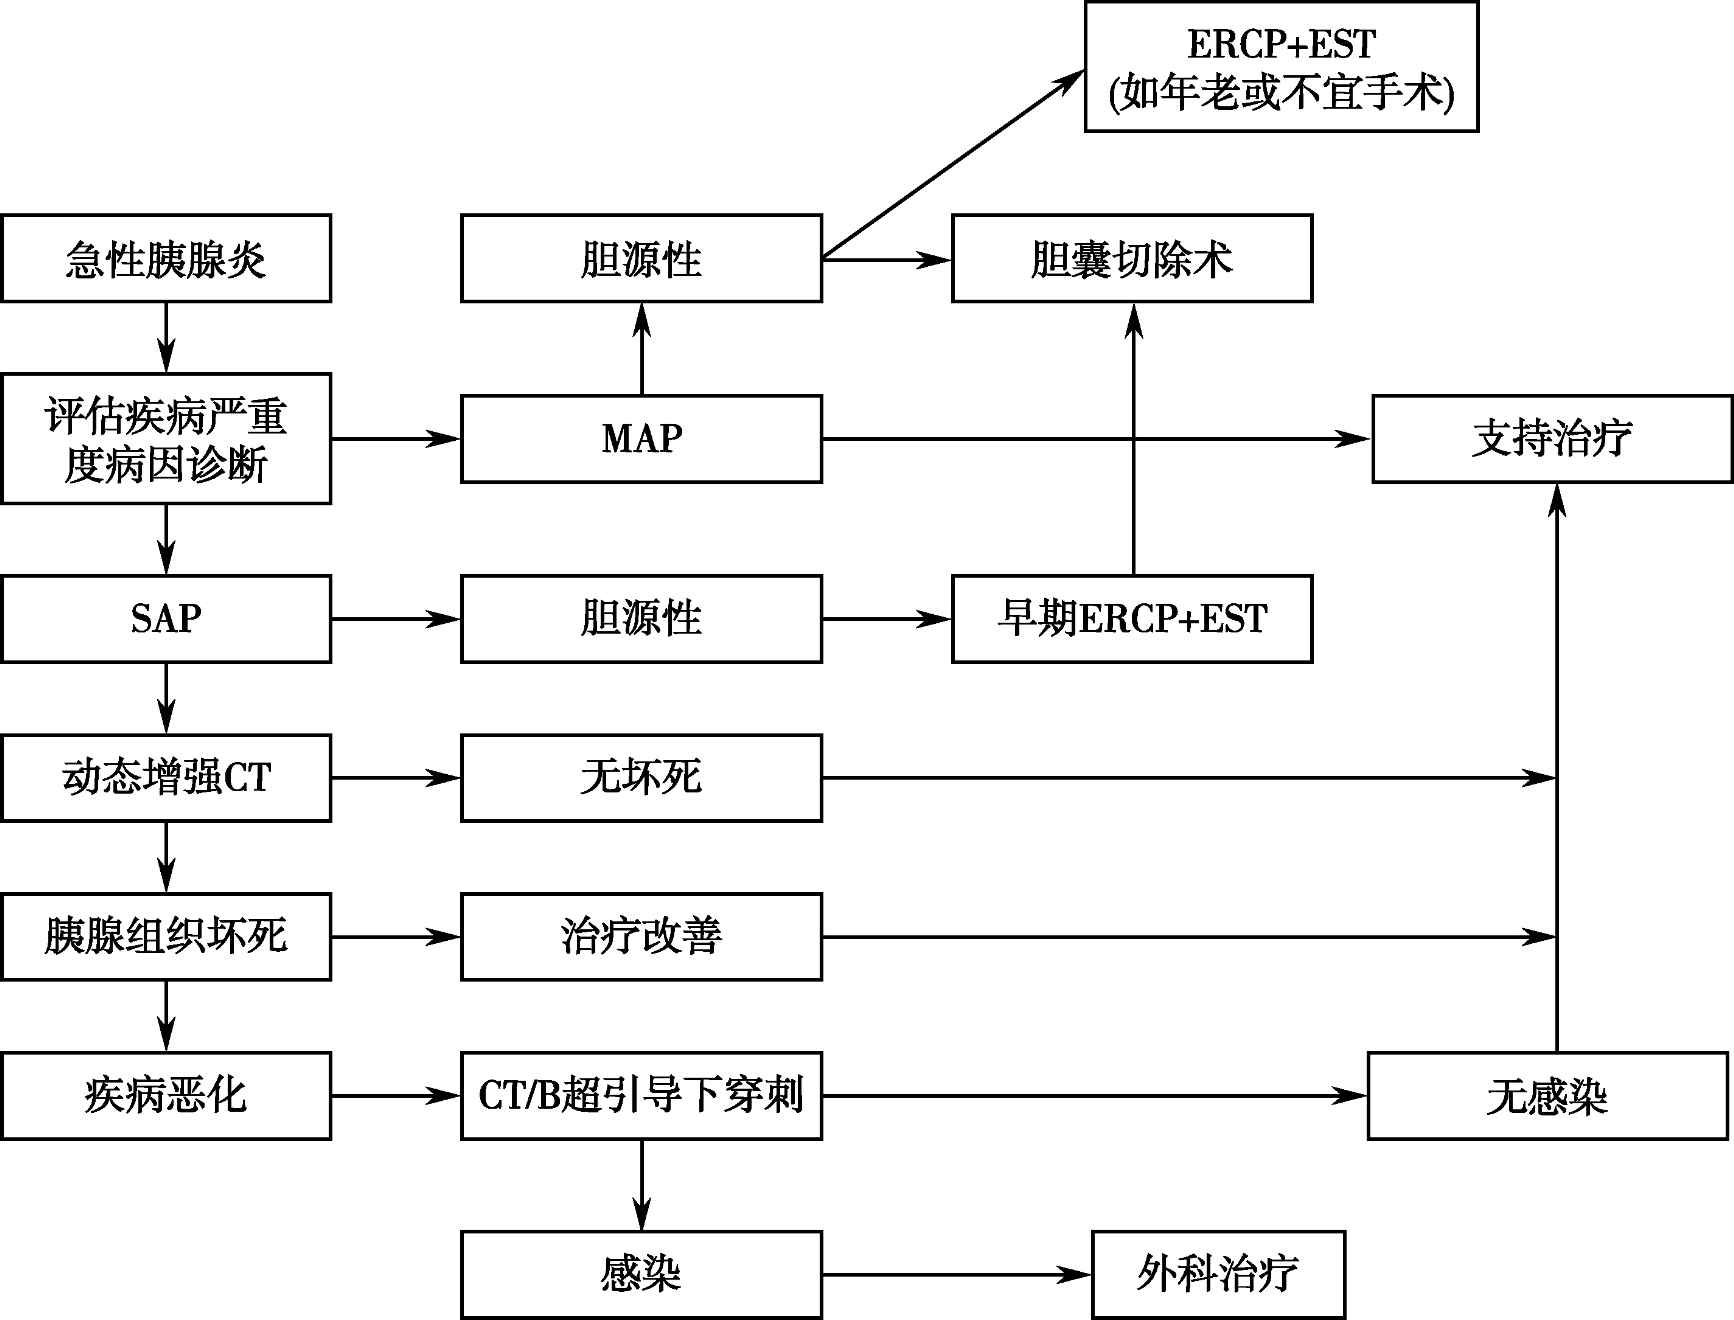
\includegraphics[width=4.75in,height=3.61458in]{./images/Image00488.jpg}
 \captionsetup{justification=centering}
 \caption{急性胰腺炎临床处理流程}
 \label{fig115-1}
  \end{figure} \protect\hypertarget{text00327.html}{}{}

\hypertarget{text00327.htmlux5cux23CHP11-6-4}{}
参 考 文 献

1. 中华医学会消化病学分会胰腺疾病学组
.中国急性胰腺炎诊治指南(草案).中华内科杂志,2004,43(3):236

2. 陈灏珠 ,林果为.实用内科学.第13版.北京:人民卫生出版社,2009:2129

3. 陆再英,钟南山.内科学.第7版.北京:人民卫生出版社,2008:469

4. Heinrich S,Schafer M,Rousson V,et al. Evidence-based treatment of
acute pancreatitis:a look at established paradigms. Ann
Surg,2006,243(2):154

\protect\hypertarget{text00328.html}{}{}

\chapter{肝硬化急症}

\section{肝硬化并上消化道出血}

上消化道出血(hemorrhage of upper digestive
tract)是肝硬化门脉高压症最常见的并发症,其特征是起病突然,出血量大且易反复,内科治疗常难以控制,病情发展迅速,危及生命,病死率较高,达42\%~90\%。若抢救成功,亦会表现有进一步的肝细胞损害,导致肝功能衰竭,诱发肝肾综合征、肝性脑病等严重并发症。

\subsection{病因与发病机制}

肝硬化患者发生上消化道出血并不全是由食管胃静脉曲张破裂所致,可能是多种因素共同作用的结果。其常见的病因有:

\paragraph{食管胃底静脉曲张破裂出血(esophageal and gastric variceal}
bleeding,EGVB)

是肝硬化最常见且最凶险的并发症。食管胃底静脉曲张是门脉高压症的特征性表现,门脉高压症食管胃静脉曲张破裂出血的机制有:①“糜烂”学说(erosion
theory):该学说认为曲张静脉出血是由于黏膜炎症影响曲张静脉的牢固性,在吞咽粗糙、刺激性食物或胃食管反流时,直接损伤薄的、脆弱的静脉壁所致。②“爆裂”学说(explosion
theory):认为导致出血的主要因素是曲张静脉内过高的流体静压,导致静脉曲张的因素同样也会导致静脉破裂。目前认为,决定静脉是否破裂的因素不是压力本身,而是曲张静脉壁的张力,出血仅发生于静脉壁张力过高时。按Laplace定律,静脉壁张力与其他因素的关系可以下式表示:张力=(P\textsubscript{1}
− P\textsubscript{2} )× r/W。式中,P\textsubscript{1}
表示曲张静脉内压力,P\textsubscript{2}
代表食管腔内压力,r为曲张静脉半径,W为静脉壁厚度。该式显示:曲张静脉愈粗,其内压力愈高,加于静脉壁上张力也愈大。粗的(Ⅳ度)、壁薄的(内镜下蓝色基调、红色征阳性)静脉曲张,即使静脉内压不太高,也易破裂。总之,导致静脉破裂出血的因素是相互关联的,首先,门脉高压促发侧支循环形成和食管胃静脉曲张。持续门脉高压合并血流量增加,导致曲张静脉不断扩张增粗,静脉壁也逐渐变薄,从而使静脉壁张力提高到“高危”水平,此时,任何能进一步导致曲张静脉内压升高,静脉管径进一步变大的因素,如恶心、呕吐或体位不当促使腹内压突然升高而使曲张静脉破裂出血。食管胃静脉曲张破裂出血是肝硬化最常见的致死性并发症,约有50\%的肝硬化患者存在食管胃底静脉曲张,每年静脉曲张破裂出血的发生率为5\%~15\%。胃食管静脉曲张与肝病的严重程度有关,Child
A级仅40\%有食管胃底静脉曲张,而Child
C级85\%存在食管胃底静脉曲张。无静脉曲张的肝硬化患者每年静脉曲张的发生率为8\%,小静脉曲张的患者每年有8\%发展成为大静脉曲张。

\paragraph{门脉高压性胃病(portal hypertensive gastropathy,PHG)}

肝硬化时胃黏膜可见淤血、水肿和糜烂,呈马赛克或蛇皮样改变,称为门脉高压性胃病(PHG),是引起肝硬化患者非曲张静脉破裂出血的主要原因,其发生率与门脉高压的严重程度相关,据报道PHG出血占门脉高压性上消化道出血的10\%~60\%。目前认为肝硬化门脉高压合并PHG的发病机制主要涉及到以下方面:①门脉高压时合并低氧血症,导致胃黏膜血管扩张和毛细血管网开放,加重胃黏膜充血;②胃黏膜血流量减少,营养物质丢失和代谢障碍,胃内H\textsuperscript{+}
逆弥散增加,胃黏膜易发生糜烂出血;③肝硬化门脉高压时胃肠道水肿、缺血、缺氧,通透性增加,有利于内毒素吸收,且肝脏对内毒素的清除能力减退,引起内毒素血症,可引起胃黏膜血管扩张充血和出血;④肝功能减退时,肝脏合成凝血因子减少,凝血功能障碍,加重胃黏膜糜烂出血;⑤门脉高压时胃黏膜内毛细血管扩张、扭曲,形成动静脉短路及动脉瘤,易破裂出血。PHG病变主要累及胃底和近端胃体,与静脉曲张破裂出血相比,此类患者出血量一般较小,部分患者以黑便为首发症状,出血前患者可有上腹部疼痛或灼热感,有的可查询到服用有关药物史。

\paragraph{肝源性溃疡(hepatic ulcer,HU)}

肝硬化患者溃疡的发病率可明显增高,门脉高压是其发病的确切危险因子,其发生与门静脉高压致使胃黏膜保护机制下降,促酸分泌物质如组胺、5-羟色胺、胃泌素等在肝脏的灭活下降及内毒素血症有关。HU的发生率是普通胃、十二指肠溃疡的2~7倍,HU患者的疼痛症状多不明显,常被肝病本身的消化道症状所掩盖,许多患者是在并发出血后行急诊胃镜检查时才发现有溃疡存在。

\paragraph{其他}

食管胃底曲张静脉破裂、门脉高压性胃病、肝源性溃疡是引起肝硬化患者上消化道出血最常见的三个原因,其他少见的原因还有:异位静脉曲张、胃窦毛细血管扩张症及肝性胃肠功能衰竭等,其原因均与门静脉压力有关。

此外,因肝脏合成凝血因子减少或脾功能亢进时血小板减少,和毛细血管脆性增加所导致的凝血机制异常,直接或间接参与消化道出血的发生,同时也进一步增加止血治疗的困难。

\subsection{诊断}

\subsubsection{临床表现特点}

\paragraph{肝功能减退和门脉高压的症状和体征}

患者多有慢性肝病的基础,有消瘦乏力、食欲减退、上腹部饱胀不适、恶心呕吐、腹泻甚至黄疸等肝功能减退的症状;有腹水、脾肿大、腹壁与脐周静脉曲张、痔核形成等门脉高压、侧支循环建立与开放的表现。

\paragraph{消化道出血的表现}

呕血与黑便,是上消化道出血的特征性表现。出血量大或出血速度较快时会出现呕新鲜血或血块,粪便可呈暗红色甚至鲜红色。

\paragraph{失血性周围循环衰竭和贫血}

急性大量失血由于循环血量迅速减少而导致周围循环衰竭,一般表现为头昏、乏力、心悸,严重时出现晕厥甚至休克状态。急性大量出血后均有失血性贫血,一般在出血后3~4小时出现,多为正细胞正色素性贫血。

\paragraph{并发症}

肝硬化上消化道出血的患者极易出现水电解质平衡紊乱、自发性腹膜炎、肝性脑病及肝肾综合征等严重的并发症。

\subsubsection{实验室检查和其他检查}

\paragraph{血常规}

有轻重不等的贫血表现,脾功能亢进时还可伴有白细胞和血小板计数的减少。

\paragraph{肝功能试验}

多有肝功能异常的表现,转氨酶可有不同程度的升高,一般以ALT升高较为显著,肝细胞严重坏死时可有AST的明显升高;血清总蛋白正常、降低或增高,但白蛋白降低,球蛋白增高,白/球比例倒置;血清胆红素水平有不同程度的升高;胆固醇酯低于正常;凝血酶原时间有不同程度的延长,经注射维生素K亦不能纠正;细胞外基质增加,血清Ⅲ型前胶原肽(PⅢP)、透明质酸、层粘连蛋白等浓度常增高。

\paragraph{病原学检查}

病因为病毒性肝炎者,乙型、丙型或乙型加丁型肝炎病毒标记呈阳性反应。

\paragraph{影像学检查}

食管静脉曲张时行食管吞钡检查可显示虫蚀样或蚯蚓状充盈缺损,胃底静脉曲张时可见菊花样充盈缺损。CT和MRI检查可显示肝左、右叶比例失调,右叶萎缩,左叶增大,肝表面不规则,脾大,腹水等征象。超声显像亦可显示肝大小、外形改变和脾大,门静脉高压者门静脉主干内径>
13mm,脾静脉内径>
8mm,应用多普勒检查尚能检测门静脉的血流速度、方向和血流量。

\paragraph{内镜检查}

是诊断的金标准,能在直视下明确出血的原因,患者应在建立静脉通道,充分扩张血容量,有备血及相应止血治疗措施下及早进行内镜检查,明确出血的原因和部位。肝硬化并上消化道出血患者常见的内镜下表现有:

\hypertarget{text00328.htmlux5cux23CHP11-7-1-2-2-5-1}{}
(1) 食管静脉曲张(EV):

内镜下EV的定义:即食管内注气扩张,消除正常黏膜皱襞后,可见有向腔内突出的静脉为曲张静脉。2000年3月中华消化内镜学会参照日本门脉高压研究会标准制订了我国食管胃底静脉曲张内镜诊断标准,是目前我国应用较为广泛的内镜下EV诊断标准。该诊断标准主要根据食管静脉曲张内镜下形态(F)、曲张静脉部位(L)、基本色调(C)、红色征(RC)及有无伴发食管炎进行描述和判断。①食管静脉曲张内镜下形态(F):EV消失为F\textsubscript{0}
,EV呈直线形或略有迂曲描述为F\textsubscript{1}
,EV呈蛇形迂曲隆起为F\textsubscript{2}
,EV呈串珠状、结节状或瘤状为F\textsubscript{3}
;②曲张静脉的部位(L):以其与门齿的距离分为食管上段(LS,距离门齿15~25cm),食管中段(LM,距离门齿25~32cm)和食管下段(LI,距离门齿32~40cm);③曲张静脉的基本色调:分为白色和蓝色,数条静脉可能不一致,以最粗的色调为代表。白色曲张静脉(CW)与正常黏膜色泽一致,蓝色曲张静脉(CB)呈现与周围黏膜明显不同的蓝色,与CW相比多有紧满感。④红色征(RC):可表现为红斑、红色条纹或血泡样改变。无红色征为RC(−),有红色征为RC(+)。⑤是否伴发食管炎:主要指糜烂,有糜烂为E
+,无者为E。按照EV的形态和出血的危险程度,中华消化内镜学会建议将EV分为轻、中、重3级(表\ref{tab116-1})。

\begin{table}[htbp]
\centering
\caption{食管静脉曲张分级标准}
\label{tab116-1}
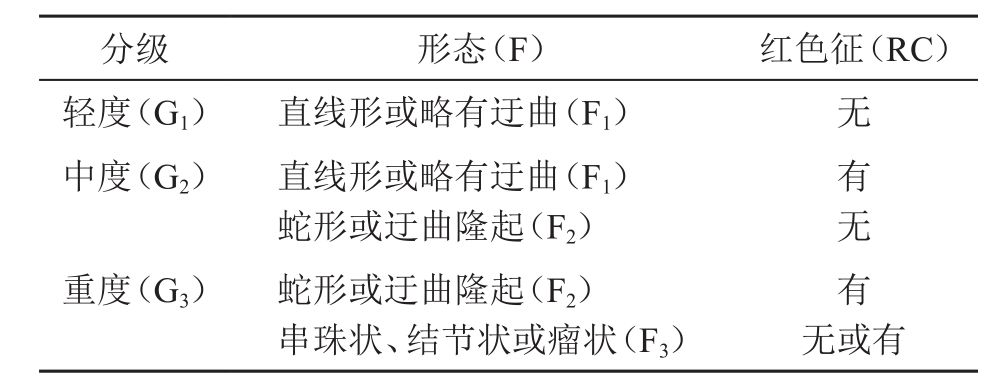
\includegraphics[width=3.29167in,height=1.27083in]{./images/Image00489.jpg}
\end{table}

2007年美国肝病研究学会实践指南建议尽可能简化曲张静脉的分级
,可简单根据曲张静脉的大小分为两类,以直径为5mm为分界线,>
5mm为大曲张静脉,< 5mm为小曲张静脉。

\hypertarget{text00328.htmlux5cux23CHP11-7-1-2-2-5-2}{}
(2) 胃底静脉曲张(GV):

5\%~33\%门静脉高压患者存在胃静脉曲张,其发生率低于食管静脉曲张。胃底静脉曲张根据直径分为大、中、小三种,分别为>
10mm,5~10mm和<
5mm。胃底静脉曲张常根据与食管静脉曲张关系和曲张静脉在胃的部位进行分类,胃食管静脉曲张(GOV)是由食管静脉曲张发展而成,分为两个类型,最常见的是GOV1型,即曲张静脉沿胃小弯延伸,是食管曲张静脉的延续而来。GOV2型从胃底沿胃大弯呈更长和更大的盘曲延伸。无食管静脉曲张的单纯胃静脉曲张(IGV)也被分为两型,1型(IGV1)见于胃底部,且形态更扭曲和复杂;2型(IGV2)见于胃体,胃窦或幽门附近。IGV1型胃底部静脉曲张患者需排除脾静脉血栓的存在。

\hypertarget{text00328.htmlux5cux23CHP11-7-1-2-2-5-3}{}
(3) 门脉高压性胃病(PHG):

内镜下表现为各种形态的充血性红斑(尤其是蛇皮征、马赛克征、樱桃红斑)和糜烂,伴或不伴有出血。Papazian等描述PHG的“特征性胃镜图像”为一种主要位于胃近端,有淡黄色网格镶嵌的多发性小红斑,类似于马赛克,故称之为“马赛克征”。

\hypertarget{text00328.htmlux5cux23CHP11-7-1-2-2-5-4}{}
(4) 其他:

常见的内镜表现还包括消化性溃疡、胃窦毛细血管扩张症等。

\paragraph{超声内镜(EUS)检查}

食管静脉曲张的超声内镜声像图表现为黏膜或黏膜下层的无回声结构,沿食管走行呈管状分布,可显示胃镜不能发现的食管周围和胃周围侧支静脉扩张现象。

对于食管静脉曲张患者,内镜是首选的检查方法,由于EUS检查时间较长,有引起静脉破裂出血的危险,一般不列为常规检查。其检查的适应证应予控制,主要在以下几个方面:①辅助诊断及分级;②观察食管周围侧支静脉曲张情况,侧支静脉扩张预示有出血危险性;③曲张静脉硬化治疗或套扎术后的追踪观察和疗效判断。

\paragraph{门脉高压的评估}

由于肝静脉压力梯度(HVPG)与门静脉压之间有良好的相关性,故HVPG常用于门静脉压的评估及治疗疗效的判断。将测压导管经股静脉、肘静脉或颈静脉送入肝静脉开口处测得游离肝静脉压(FHVP),进一步将导管向肝静脉深处送入至导管嵌入肝静脉测得肝静脉嵌塞压(WHVP)。WHVP
− FHVP =
HVPG。其变化值随时间推移对食管胃底静脉曲张的进展,破裂出血风险及死亡均有预测价值。

\subsubsection{诊断注意事项}

患者有肝病病史,在肝功能减退和门脉高压的基础上,出现呕血、黑便或便血的消化道出血表现,肝硬化并上消化道出血的诊断一般不难明确。

食管胃底静脉曲张破裂出血也是失代偿期肝硬化的严重表现,因此,此类患者常同时有严重肝病的表现。如腹水、脾肿大、腹壁与脐周静脉曲张,痔核形成等门脉高压、侧支循环建立与开放的表现;以及消瘦、纳差、出血倾向、贫血、蜘蛛痣与肝掌等肝硬化的表现。同时,对肝脏储备功能的评估不但有助预后评估,且对治疗方案的选择具有重要意义,临床常用Child-Pugh分级来评估(表\ref{tab116-2}\footnote{在PBC患者评分时对SB的标准提高:SB <68μmol/L,1分;68~170μmol/L,2分;> 170μmol/L,3分}),总分:A级≤6分,B级7~9分,C级≥10分。注意:对原发性胆汁性肝硬化(primary
biliary cirrhosis,PBC)患者评分时,总胆红素(SB)水平相应提高。

\begin{table}[htbp]
\centering
\caption{肝硬化患者 Child-Pugh分级标准}
\label{tab116-2}
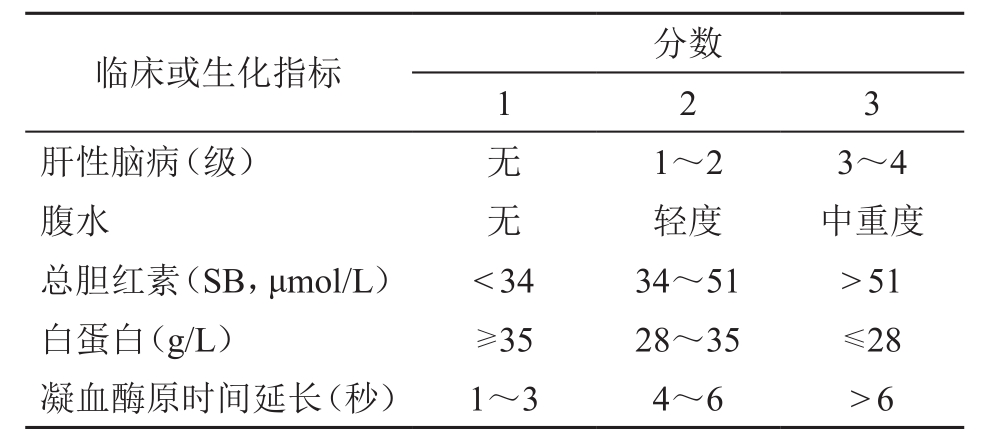
\includegraphics[width=3.30208in,height=1.45833in]{./images/Image00490.jpg}
\end{table}



诊断关键在于出血病因的明确,食管胃底曲张静脉破裂、门脉高压性胃病、肝源性溃疡是引起肝硬化患者上消化道出血三个最常见的原因,其他少见的原因还有:异位静脉曲张、胃窦毛细血管扩张症及肝性胃肠功能衰竭等。在诊断过程中,要重视病史和体征在病因诊断中的作用,一般在肝功能代偿相对良好的患者,发生急性大出血,不伴应激因素存在时,多数为静脉曲张破裂出血;患者肝功能减退明显,而出血量相对较少,或同时有应激因素(感染、肝肾综合征)存在时,应考虑非静脉曲张破裂出血(门脉高压性胃病、肝源性溃疡、肝性胃肠功能衰竭等)。

内镜检查是病因诊断的关键,能直接发现病变的性质、部位及程度,应尽早在出血后24~48小时内进行,并备好止血的药物和器械,对于出血量大的患者应先迅速纠正循环衰竭,待血红蛋白上升至70g/L后再进行内镜检查,危重患者内镜检查时应进行血氧饱和度和心电、血压的监护。

肝硬化门静脉高压食管胃静脉曲张出血的防治共识(2008,杭州)关于EGVB继续出血或再出血的评估:①提示EGVB出血未控制的征象:72小时内出现以下表现之一者为继续出血。6小时内输血4个单位以上,生命体征不稳定。收缩压<
70mmHg,HR > 100次/分或心率增加> 20
次/分;间断呕血或便血,收缩压降低20mmHg以上或心率增加>
20次/分,继续输血才能维持Hb含量稳定;药物或内镜治疗后新鲜呕血,在没有输血的情况下,Hb含量下降30g/L以上。②提示EGVB再出血的征象:出现以下表现之一者为再出血。出血控制后再次有活动性出血的表现(呕血或便血;收缩压降低20mmHg以上或心率增加>
20
次/分;在没有输血的情况下,Hb含量下降30g/L以上)。早期再出血:出血控制后72小时~6周内出现活动性出血。迟发性再出血:出血控制6周后出现活动性出血。

\subsection{治疗}

治疗原则是迅速补充血容量,纠正失血性休克,降低门脉高压和及时止血,防治肝性脑病等并发症。

\subsubsection{一般处理及重症监护}

\paragraph{休息}

绝对卧床休息、保持安静、保持呼吸道通畅,基于站立位比平卧位时肝血流量会减少20\%~30\%,而肝硬化患者比正常人肝血流量要减少20\%~40\%,因此确保肝脏血流量充足,保持静卧是改善肝循环状态最有效的治疗方法。烦躁不安时可注射小剂量地西泮(安定)、东莨菪碱,禁用吗啡、水合氯醛及速效巴比妥类药物。

\paragraph{吸氧}

可改善失血引起的肝脏及大脑的缺氧状态,对预防肝性脑病有利。

\paragraph{积极补充血容量}

谨慎快速扩充血容量,维持血流动力学稳定和血红蛋白达80g/L。即恢复所有丢失的血液和门脉压力水平。但门脉压力高于基线水平会引起再出血及病死率增加。应避免输入过多含钠溶液,以免增加静脉曲张破裂出血,加重或诱发腹水及血管外液体积聚。

\paragraph{禁食 、灌肠}

宜在出血停止后24~48小时才能进食流质。为预防肝性脑病,暂禁蛋白质食物,口服乳果糖30~100ml/d,使肠道pH降低,抑制氨的吸收;也可清洁灌肠后(忌用碱性溶液)用食醋30~50ml加水100~200ml保留灌肠以排除肠内积血和酸化肠道。

\paragraph{严密观察病情}

包括:①观察神志、血压、脉搏、呼吸,肢体是否温暖,皮肤与甲床色泽情况;②记录出血量与尿量;③定期复查RBC、Hb、Hct和BUN等;④应注意:测定中心静脉压或肺动脉嵌塞压虽然有助于判断患者的心血管状态,但在肝硬化门脉高压患者,由于外周血管阻力障碍,内脏血管床内血潴留增加,以致测出中心静脉压或肺动脉嵌塞压往往较低,其结果不能反映患者真正的血容量状态。

\subsubsection{药物治疗}

在活动性EGVB时,应首选药物治疗或药物联合内镜下治疗。目前认为有效的止血药物主要有生长抑素及其类似物和血管加压素及其类似物。

\hypertarget{text00328.htmlux5cux23CHP11-7-1-3-2-1}{}
(一) 生长抑素及其类似物

生长抑素及其类似物能选择性地直接作用于内脏血管平滑肌
,使内脏循环血流量降低,从而减少门脉及其侧支循环血流量,降低门静脉压。该类药物止血效果肯定,因不伴全身血流动力学改变,故短期使用几乎没有严重不良反应,已成为治疗EGVB最常用药物。常用的品种有:

\paragraph{14肽天然生长抑素(somatostatin,思他宁)}

用法为首剂250μg静脉缓注,继以250μg/h持续静脉滴注,维持3~5天;如仍有出血,可增加剂量至500μg/h维持。本品半衰期极短,注射后2分钟作用消失,应注意滴注过程中不能中断,若中断超过5分钟,应重新注射首剂。

\paragraph{奥曲肽(octreotide,善得定,sandostatin)}

是8肽的生长抑素类似物,半衰期较天然生长抑素长30倍,常用量为首剂50~100μg静脉缓注,继以25~50μg/h持续静脉滴注,首次控制出血率为85\%~90\%,无明显不良反应,持续应用3~5天或更长时间。

\paragraph{伐普肽(vapreotide)}

是新近人工合成的生长抑素类似物,用法为起始剂量50μg静脉缓注,继以50μg/h持续静脉滴注。生长抑素及其类似物与内镜治疗联合应用,效果优于单一药物或内镜治疗。

\hypertarget{text00328.htmlux5cux23CHP11-7-1-3-2-2}{}
(二) 血管加压素及其类似物

血管加压素及其类似物也是治疗食管静脉曲张破裂出血的常用药物
,通过收缩全身及肠系膜动脉、肝动脉等内脏血管,减少门脉血流量,降低曲张静脉压力,达到止血的目的。

\paragraph{垂体后叶素}

含血管加压素(vasopressin,VP)和催产素(oxytocin)。VP能直接收缩内脏血管床的小动脉和毛细血管前括约肌,增加毛细血管前、后阻力之比值,使内脏循环血容量减少,从而减少门静脉血流量;能收缩肝动脉以减少其流量;使肝窦内压暂时性下降而致门静脉压降低;能明显降低胃左静脉和食管曲张静脉的血流灌注,直接减低曲张静脉壁的张力和压力。VP大部分在肝、肾破坏,故应维持用药。此外,本药尚有升高血压,增强肠蠕动,排出积血,减轻氮质血症与吸收热的作用,可作为休克治疗的辅助药物。

垂体后叶素虽能减少门静脉血流量、门体侧支循环血流量和曲张静脉压力,止血有效率60\%~80\%,但病死率未获降低,且不良反应较多(如腹痛、血压升高、心律失常、心绞痛,严重者可致心肌梗死)。加用硝酸甘油可增强血管加压素的降门脉压力作用,减少其心血管副作用,提高止血有效率和耐受性,对存活率无影响,且联用硝酸甘油后的不良反应仍高于特利加压素、生长抑素及其类似物。为减少不良反应,静脉持续使用最高剂量血管加压素的时间≤24小时。血管加压素的推荐用法是0.2U/min静脉持续滴注,视治疗反应,可逐渐增加剂量至0.4U/min(目前国内所用垂体后叶素含等量加压素与缩宫素)。联用硝酸甘油(其剂量为每15~30分钟舌下含0.4~0.6mg,或以10~50μg/min静滴)。冠心病、高血压、孕妇、肾功能不全者禁用。

\paragraph{三甘氨酰赖氨酸加压素(又名特利加压素,terlipressin)}

是血管加压素的合成类似物,可持久有效地降低HVPG、减少门静脉血流量,且对全身血流动力学影响较小。止血效果肯定,不良反应少。其止血效果优于血管加压素,与生长抑素、血管加压素联用硝酸甘油、气囊压迫和内镜治疗相当。特利加压素的推荐起始剂量为每4小时静注2mg,出血停止后可改为每日2次,每次1mg,一般维持5天,以预防早期再出血。

\hypertarget{text00328.htmlux5cux23CHP11-7-1-3-2-3}{}
(三) 血管扩张剂

血管扩张剂能使门静脉分支和肝内血管扩张
,致门静脉压下降;同时由于动脉压下降,反射性引起内脏动脉收缩,使门脉血流量减少,从而明显降低门脉压。目前主要与缩血管药物合用或止血后预防再出血,不主张在大出血时单独应用血管扩张剂。

\paragraph{硝酸甘油(nitroglycerin,NTG)}

为快作用的硝酸酯类制剂。常在静脉滴注VP后或同时应用。其剂量为每15~30分钟舌下含0.4~0.6mg,或静滴10~40μg/min。NTG与VP合用可以避免或减轻VP的全身性血管收缩所致副作用。

\paragraph{酚妥拉明(regitine)}

为α肾上腺素能受体阻滞剂。在静滴垂体后叶素0.2~0.4U/min的同时,静滴本品0.1~0.3µg/min,出血控制后减量维持,止血12小时后停药。

\hypertarget{text00328.htmlux5cux23CHP11-7-1-3-2-4}{}
(四) 抑酸药物

制酸剂可有效提高胃内
pH,既可促进血小板聚集和纤维蛋白凝块的形成,又可避免血凝块过早溶解,有利于止血和预防再出血,是目前治疗门脉高压性出血的基本药物。临床上常用的制酸剂主要包括H\textsubscript{2}
受体拮抗剂(H\textsubscript{2}
RA)和质子泵抑制剂(PPI)两大类。其应用参见本书第13章“消化道出血”。

\hypertarget{text00328.htmlux5cux23CHP11-7-1-3-2-5}{}
(五) 去甲肾上腺素的局部应用

去甲肾上腺素可使胃肠道局部血管收缩
,减少血流量而达到止血。方法是先经胃管将胃内血块清除后,以去甲肾上腺素16mg溶入200ml生理盐水内,口服或经胃管注入,20~30分钟后抽取胃内容物,观察有无出血。如出血未止,可每4小时一次。此法简便,局部用药不引起血压升高,如使用时间不长,不会引起胃肠道缺血。老年患者慎用。

\hypertarget{text00328.htmlux5cux23CHP11-7-1-3-2-6}{}
(六) 抗生素的应用

活动性出血时常存在胃黏膜和食管黏膜炎性水肿,预防性使用抗生素有助于止血,并可减少早期再出血及预防感染。荟萃分析表明,抗生素可通过减少再出血及感染提高存活率。因此,使用抗生素预防和(或)治疗细菌感染,是治疗EGVB的一个不可缺少的部分,应及时给予,持续7~10天。静脉途径或口服给药效果无差别,常开始静脉用药随后予以口服维持。大多数首选喹诺酮类抗生素,对喹诺酮类耐药者也可使用头孢类抗生素。

\hypertarget{text00328.htmlux5cux23CHP11-7-1-3-2-7}{}
(七) 止血药物

确切作用尚未证实
,不能作为一线药物使用,对有凝血功能障碍者,可静脉注射维生素K\textsubscript{1}
;为防止继发性纤溶,可使用氨甲苯酸(止血芳酸)等抗纤溶药物;云南白药等中药也有一定的疗效。此外还可使用局部止血药,如口服凝血酶等。应避免滥用止血药。

\hypertarget{text00328.htmlux5cux23CHP11-7-1-3-2-8}{}
(八) 输血或血制品

肝硬化患者由于肝功能不良和脾功能亢进
,多合并有血小板减少和(或)凝血机制障碍。对于合并消化道出血的患者,可根据个体情况选择输注新鲜血、血小板或新鲜冰冻血浆,可纠正患者贫血,补充血小板和凝血因子有助于止血,并可以改善患者一般情况。

\subsubsection{内镜治疗}

内镜治疗的目的是控制急性食管静脉曲张出血,并尽可能使静脉曲张消失或减轻以防止其再出血。一般经药物治疗(必要时加气囊压迫)大出血基本控制,患者基本情况稳定,在进行急诊内镜检查(出血后24~48小时内)同时进行治疗。方法有内镜下硬化剂注射治疗(endoscopic
injection sclerotherapy,EIS)、内镜下曲张静脉套扎治疗(endoscopic
variceal
ligation,EVL)和内镜下组织黏合剂注射治疗,均是治疗EGVB的一线疗法,各医院可根据具体情况选用。

\paragraph{内镜下硬化剂注射治疗(EIS)}

EV硬化治疗的适应证有:①急性EV破裂出血;②既往有EV破裂出血史行预防性注射;③外科手术后EV再发者;④内科药物治疗失败,又不适于手术治疗者。重度黄疸、休克、肝性脑病患者不适于此项治疗。

硬化剂治疗的机制在于:硬化剂注射入静脉后首先破坏血管内皮,引起白细胞浸润,形成血栓性静脉炎,同时出现成纤维细胞增生,一周左右发生局部组织坏死,重者形成溃疡,于10~14天出现肉芽组织,3~4周发生纤维化,血管闭塞。

常用的硬化剂有5\%鱼肝油酸钠(sodium
morrhuate)、5\%油酸氨基乙醇(ethanolamine
oleate)、1\%乙氧硬化醇(aethoxysklerol)、1.5\%十四烷基磺酸钠(sodium
tetradecyl sulfate)及纯酒精(absolute
alcohol)等。操作方法有单纯注射法、内镜附加气囊注射法,内镜附加外套管注射法。注射方法有静脉内注射和静脉旁加黏膜下注射。

第一次硬化治疗后可行第二次、第三次硬化治疗,直至曲张静脉消失或基本消失,每次硬化治疗间隔时间1~2周左右,疗程结束后一个月复查胃镜,以后每3~6个月复查一次胃镜,曲张静脉再生或复发出血时需要追加治疗。

EIS急性止血的成功率为81\%~98\%,曲张静脉的根除率为80\%~93\%,出血的复发率在19\%~50\%。不同的Child-Pugh分级患者疗效不同,EIS对Child-Pugh分级A、B食管静脉曲张患者有确切疗效,对Child-Pugh分级C患者疗效相对较差。EIS的并发症主要有胸骨后疼痛、短暂发热、注射部位出血、食管溃疡及狭窄、纵隔、胸腔积液、异位栓塞等。

\paragraph{内镜下曲张静脉套扎治疗(EVL)}

EVL出现于20世纪80年代,其原理就是将套扎的皮圈拉开后直接放在与内镜前端紧密连接的透明帽上,利用负压将曲张静脉直接吸引至透明帽内,而后将皮圈退出,将皮圈直接扎于曲张静脉上,从而达到结扎曲张静脉的目的。利用该方法将曲张静脉分段进行套扎,就可使曲张静脉血流中断,形成血栓,达到治疗静脉曲张的目的。

EVL主要适应于存在食管曲张静脉出血,曲张的食管静脉直径小于1cm。一般一次套扎5~12处,在进行EVL治疗时要求一次将能见到的所有曲张静脉全部结扎完毕,以免遗漏未结扎的静脉压力增高导致出血。一般间隔2周,进行下次套扎治疗。EVL的主要并发症为吞咽困难、胸骨后疼痛,多在1~3天内缓解,严重的并发症为早期结扎环脱落导致致命性的大出血。

\paragraph{胃底曲张静脉的治疗}

十年前,胃静脉曲张作为上消化道出血的原因并不显得重要,因为不论食管或胃静脉曲张出血均采用门体分流术治疗。近十年来,由于EIS、EVL的成功应用,较少采用门体分流术,胃静脉曲张发生率和出血率才被人们重视。

胃静脉曲张的治疗原则上以手术治疗为主,但对急诊的胃静脉曲张出血的治疗可首选组织黏合剂(组织胶)治疗,为手术创造条件。组织胶注射入血管内接触到血液时会在1/20秒内发生聚合反应,形成固体,堵塞球形扩张的曲张静脉,从而迅速闭塞曲张静脉,起到止血的作用。常用的组织胶有氰丙烯酸盐及TH胶等。主要并发症有排胶引起的近期再发出血,肺动脉和门静脉栓塞,但发生率较低。

\paragraph{联合治疗}

EVS联合EIS治疗近年来文献报告甚多,临床上常采用套扎+硬化序贯之治疗,一般在两次套扎治疗后再对残留的小曲张静脉行硬化治疗。

\subsubsection{气囊压迫止血}

将三腔双囊管或四腔双囊管插入上消化道内,将胃气囊和(或)食管气囊充气以压迫曲张静脉达到止血目的,是一种行之有效的急救方法,其疗效确切,对控制急性出血成功率高。但患者痛苦大、并发症多(如吸入性肺炎、窒息、食管炎、食管黏膜坏死、心律失常等),气囊放气后再出血率高。目前已不推荐气囊压迫作为首选止血措施,其应用宜限于药物不能控制出血时作为暂时止血用,以赢得时间去准备其他更有效的治疗措施。进行气囊压迫止血时,应根据病情8~24小时放气1次,拔管时机应在血止后24小时,一般先放气观察24小时若仍无出血即可拔管。此外,在三腔二囊管压迫止血时特别要注意保护好呼吸道。用法参见本书第141章“三腔二囊管压迫止血术”。

\subsubsection{放射性介入治疗}

放射介入疗法如TIPS可有效地控制出血,但明显增加肝性脑病的危险,适用于对药物和内镜治疗难以控制的曲张静脉出血和等待肝移植的患者。

\paragraph{胃冠状静脉栓塞术}

是治疗门脉高压食管胃底静脉曲张出血的有效方法,但该疗法不能降低门脉压力甚至使门脉压力升高,在预防远期再出血方面疗效不满意,因此常联合其他的方法如部分脾静脉栓塞术或经颈静脉肝内门体分流术等方法同时进行。临床应用时应严格掌握适应证:用于临床保守治疗或内镜下治疗无效的食管胃底静脉曲张破裂出血,治疗主要在出血期进行。有明显出血倾向或终末患者为禁忌。本方法在操作时直接门静脉造影,显示胃冠状静脉或胃短静脉以及增粗扭曲的食管静脉丛,借助导管导丝进入胃冠状静脉及胃短静脉进行栓塞治疗,先用无水乙醇10~30ml分次推注,再用高压消毒过的明胶海绵长条进行栓塞,最后用钢圈栓塞其主干。然后将导管置入脾静脉重复造影,见曲张静脉完全阻断则治疗满意。胃冠状静脉栓塞术既能使曲张血管形成血栓,又能使其主干血流完全阻断,急性出血止血率可达100\%。联合部分脾静脉栓塞术或经颈静脉肝内门体分流术可明显降低远期再出血率,与内镜下治疗相比优势在于对贲门胃底曲张静脉破裂出血也有效。

\paragraph{经颈静脉肝内门体分流术(transjugular intrahepatic portosystemic}
shunt,TIPS)

是在门腔静脉分流术的基础上产生和发展起来的一种介入治疗方法。此法经颈内静脉插入穿刺导管,通过肝右静脉,在肝实质内穿刺门静脉的左支或右支,以建立起门静脉-肝静脉通道,进而用球囊扩张通道,放入可扩张性血管支架,保持分流道通畅。TIPS将肝外门腔分流转移至肝内,可有效降低门脉压力,同时肝内分流道起到“限制性分流”的作用,血流方向为“进肝流向”,这就维持了肝脏所需的含“肝营养因子”的胰腺血流,使肝功能得到改善,属限制性门体分流术。

TIPS的适应证:①门静脉高压症食管胃底曲张静脉破裂出血经药物和内镜治疗无效而肝功能差不适于手术者;②断流术后再出血者;③门脉高压所致顽固性腹水;④肝移植术前准备;⑤断流术术前准备。TIPS术近期止血效果确切,手术成功率达90\%左右,静脉曲张的消失及基本消失率为41.4\%,总有效率为79.3\%,腹水减少或消失为62\%。但中远期效果并不理想,主要存在两个问题:①肝性脑病;②分流道狭窄,术后半年的再狭窄率为20\%~30\%,一年后再狭窄率为40.5\%~55\%。因此从门脉高压症的远期疗效考虑,TIPS不宜作为首次食管胃底曲张静脉破裂出血的首选方法。

\subsubsection{手术治疗}

急诊外科手术控制曲张静脉出血和预防再出血的效果确实,但围术期病死率高,术后肝性脑病发生率高。仅在药物和内镜治疗无效、无法施行TIPS的情况下方可使用。Child-Pugh
C级肝硬化患者不宜施行急诊外科手术。必要时可考虑肝移植。

尽管使用有效的药物及内镜治疗,但仍有约10\%~20\%的患者不能控制静脉曲张出血和早期再出血。肝静脉压力梯度大于20mmHg(出血24小时内检测)是治疗失败的预测因子。

分流手术如外科分流或TIPS作为对内镜或药物治疗失败患者的挽救治疗已被临床证实有效。

\subsubsection{防治并发症}

主要包括吸入性肺炎、肝性脑病、感染、低氧血症和电解质紊乱等,参见有关章节。

\subsection{预防}

\subsubsection{初次出血的预防}

初次出血患者的病死率高达50\%,因此对于可能发生EGVB的人群,应积极采取措施预防出血。

\paragraph{高危人群的筛查和识别}

曲张静脉出血的危险性和预后与肝病的严重程度和曲张静脉大小关系密切。肝病严重程度以肝功能Child-Pugh分级来评定。曲张静脉大小则以内镜检查来评估,推荐以下人群应施行内镜检查,以评估曲张静脉大小:①Child-Pugh
A级,伴有门静脉高压征象,尤其是血小板计数< 14 × 10\textsuperscript{9}
/L的肝硬化患者;②门静脉直径>
13mm的肝硬化患者;③Child-Pugh分级B或C级的肝硬化患者;④胆红素>
20μmol/L的原发性胆汁性肝硬化和原发性硬化性胆管炎等淤胆性疾病。对于初次内镜检查未发现食管胃静脉曲张者,应2~3年复查内镜;对于发现细小曲张静脉者,应每1~2年复查内镜;对于酗酒、严重肝功能损害和曲张静脉表面有红色征者,曲张静脉增长速度很快,应每年复查内镜。以下患者应常规予以预防干预:①肝功能Child-Pugh分级B级或C级,且曲张静脉呈Ⅱ度者;②曲张静脉呈Ⅲ度者。预防措施以药物为主,也可根据患者具体情况和医疗条件采取内镜治疗和外科手术。

\paragraph{药物治疗}

非选择性β受体阻滞剂(普萘洛尔和纳多洛尔)可收缩内脏血管和减少心输出量,降低门静脉压力梯度、减少奇静脉血流及曲张静脉压力,是预防曲张静脉出血首选的措施,可有效地预防和延缓曲张静脉初次出血和EGVB的病死率。早期应用普萘洛尔可延缓食管细小曲张静脉的增长速度。普萘洛尔起始剂量10mg,每日2次,口服,渐增至最大耐受剂量;纳多洛尔起始剂量20mg,每日1次,口服,渐增至最大耐受剂量,应长期使用。也可应用长效普萘洛尔制剂以提高患者依从性。服用普萘洛尔过程中不宜骤然停药,否则有诱发出血的危险性。应答达标的标准:HVPG下降至12mmHg以下或较基线水平下降>
20\%。若不能检测HVPG,则应使静息心率下降到基础心率的75\%或静息心率达50~60次/分。禁忌证:窦性心动过缓、支气管哮喘、慢性阻塞性肺部疾病、心功能衰竭、低血压、房室传导阻滞、胰岛素依赖性糖尿病、外周血管病变、肝功能Child-Pugh分级C级、急性出血期。单硝基异山梨酯与非选择性β受体阻滞剂联合应用,可协同降低门静脉压力,可以试用,但尚缺乏循证医学证据支持。目前不提倡单用单硝基异山梨酯预防EGVB。

\subsubsection{再出血的预防}

首次出血后存活的患者如不给予预防措施,2/3的患者可能在2个月内再次出血。因此,所有发生曲张静脉出血的患者,在控制曲张静脉活动性出血后,即应采取积极的预防措施,包括药物、内镜治疗、放射介入和外科手术等。

\paragraph{内镜治疗}

EVL和EIS可显著地降低EGVB患者的再出血率和病死率,是预防曲张静脉再出血的有效方法。一般根据患者肝功能状况选择,肝功能良好者以EIS更为多用,肝功能不佳者,则建议选择EVL。提倡在内镜治疗后短期内应用质子泵抑制剂以预防溃疡形成和促进溃疡愈合。

\paragraph{药物治疗}

药物治疗的主要目标是将反映门静脉压力的肝静脉压力梯度降至12mmHg以下或降低20\%以上,以预防再次出血。非选择性β受体阻滞剂普萘洛尔具有降低再出血率和提高存活率的效应,合用单硝基异山梨酯将进一步降低再出血率。

\paragraph{放射介入和外科手术}

Child-Pugh A或B级肝硬化患者可以采用手术治疗,Child-Pugh
C级肝硬化患者则考虑肝移植。暂无手术条件者,可先行TIPS。

EGVB的诊治流程见图\ref{fig116-1}。

\begin{figure}[!htbp]
 \centering
 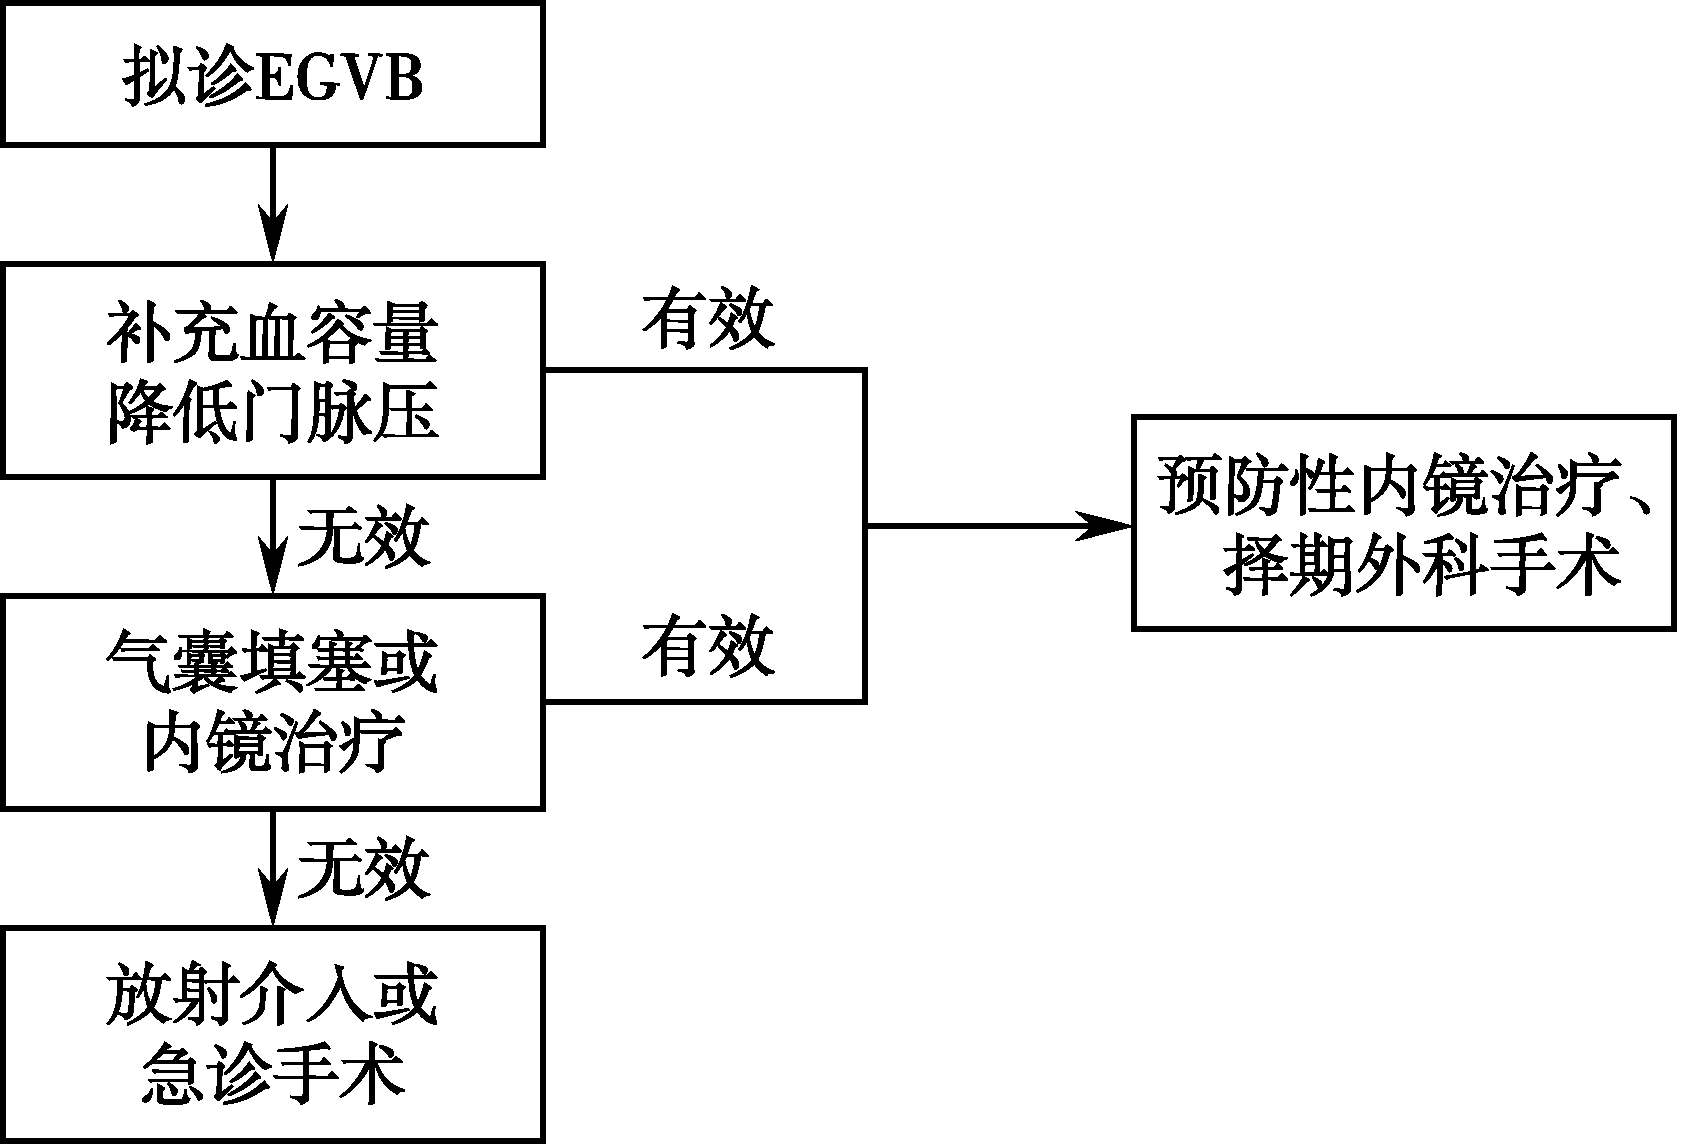
\includegraphics[width=2.8125in,height=1.90625in]{./images/Image00491.jpg}
 \captionsetup{justification=centering}
 \caption{食管胃静脉曲张出血诊治流程图}
 \label{fig116-1}
  \end{figure} \hypertarget{text00328.htmlux5cux23CHP11-7-1-5}{}
参 考 文 献

1. Garcia-tsaol. AASLD Practice guidelines. Prevention and management of
gastroesophageal varices and variceal hemorrhage in cirrhosis.
Hepatology,2007,46:922-938

2. 中华医学会消化病学分会
,中华医学会肝病学分会,中华医学会内镜学分会.肝硬化门静脉高压食管胃静脉曲张出血的防治共识(2008,杭州).中华消化杂志,2008,28(8):551

3. Dimaio CJ,Stevens PD. Nonvariceal upper gastrointestinal bleeding.
Gastrointest Endoscopy Clin N Am,2007,17:253-272

4. 中华内科杂志编委会
.食管胃静脉曲张出血的诊治建议(草案).中华内科杂志,2006,45(6):524

5.
《中华内科杂志》编委会,《中华消化杂志》编委会,《中华消化内镜杂志》编委会.急性非静脉曲张性上消化道出血诊治指南.中华消化杂志,2009,29(10):682-685.

\protect\hypertarget{text00329.html}{}{}

\section{肝硬化并自发性细菌性腹膜炎}

自发性细菌性腹膜炎(spontaneous bacterial
peritonitis,SBP)是指在腹腔及邻近组织无感染源(如腹腔脓肿、急性胰腺炎、胆囊炎、肠穿孔等)情况下发生的腹水感染,常见于肝硬化患者。有关该病的最早病例报告见于1907年,但美国学者Conn于1964年最先使用“自发性腹膜炎”这一术语。据统计在肝硬化患者SBP的发生率高达10\%~30\%,肝硬化患者并发SBP后,因其症状变化多样,诊断困难,预后较差。

\subsection{病因与发病机制}

\subsubsection{病原学}

SBP感染多来自肠道细菌,绝大多数为单一细菌感染,混合感染少见。革兰阴性与革兰阳性细菌的比例分别为70\%~80\%与20\%~30\%左右,肠源性革兰阴性菌感染最为常见,其中又以大肠杆菌为主,其次为肺炎克雷伯菌、阴沟肠杆菌等。革兰阳性菌感染则以肺炎链球菌最为常见,此外还包括肠球菌、其他链球菌以及金黄色葡萄球菌等。但金黄色葡萄球菌感染一般少见,常与接受腹腔-颈静脉分流术或腹水回输等操作有关。相对而言,腹水还保持了较高的抗厌氧菌活性,因此厌氧菌的感染率相对为低,约占总感染病例的10\%以下。

近年来随着广谱抗生素的广泛应用,SBP的细菌学及其耐药性发生了一定的变迁,表现为产生超广谱β内酰胺酶(ESBLs)阳性的大肠杆菌的感染数量有逐渐增多的趋势,约占33\%,真菌感染性SBP较前增多。最近有研究显示,在SBP抗生素药敏试验中,无耐药者只占22.5\%,至少对一种抗生素耐药的细菌(单药耐药)为77.5\%,对三类以上抗生素耐药者(多重耐药)为32.5\%。

\subsubsection{感染途径}

肝硬化腹水患者并发SBP的感染途径(即细菌来源)有:①血源性感染:SBP患者在血液和腹水同时分离出同种致病菌者可达50\%,而部分患者腹水培养尚处于阴性时,血培养已有细菌生长。此外,呼吸道、泌尿道感染时,部分可合并SBP,且同时培养出相同致病菌,也支持SBP的血源性感染。②经肠壁直接感染:即透壁假说也逐渐被认同,肠道细菌经肠壁直接感染腹水是常见途径。③胸腔内感染:可通过横膈淋巴管道到达腹腔,较为少见。④外源性感染:腹腔穿刺抽取腹水或反复排放腹水,腹部巨大脐疝伴糜烂渗出及动、静脉插管术等,有可能致SBP。

\subsubsection{发病机制}

在肝硬化失代偿期患者中,高龄、腹水低蛋白(<
10g/L)、高血清胆红素水平(>
51.3μmol/L)、消化道出血等均为SBP易患因素。SBP的发生机制并未完全明了,目前认为可能涉及到以下方面:

\paragraph{肠道细菌易位}

细菌易位,即具有繁殖活性的细菌由肠腔内原居住处迁移至肠系膜淋巴结和其他肠道部位,被认为是导致SBP的主要机制之一。正常人除回肠有少量细菌生长外,在此以上部位均无细菌生长,而肝硬化患者存在有肠道内菌群上移,在小肠上部、空肠、回肠皆可有大肠杆菌繁殖。肝硬化门脉高压引起的肠壁淤血水肿以及腹泻、肠道黏膜感染等均使肠黏膜防御功能下降和肠壁通透性升高,肠腔内细菌可直接穿过肠壁进入腹腔而感染。此外,上消化道出血时给患者使用垂体后叶素,可使肝硬化患者在内脏淤血水肿的基础上,因内脏动脉收缩致血流降低,组织缺氧和酸中毒,使业已减弱的肠黏膜屏障进一步遭破坏,以致肠内细菌进入血液或直接穿过肠壁进入腹腔。对肠腔内、肠系膜淋巴结以及腹水中的细菌进行分子生物学的鉴定,发现细菌的DNA指纹符合率高。因此肠道细菌过度繁殖并从肠道到腹腔的易位是造成SBP的一种既简单又最具可能性的解释。

\paragraph{侧支循环开放}

肝脏对清除血液循环的细菌起着重要作用,这主要是因肝内丰富单核巨噬细胞系统。肝硬化门脉高压患者,由于肝内外功能上和解剖上的分流,使得经胃肠道进入血液循环的细菌,能绕过肝脏的单核巨噬细胞,进入体循环并长期存在,已证明肝硬化患者可使80\%的门脉血通过肝内、外门体分流直接进入体循环。

\paragraph{机体防御功能低下}

①肝内单核巨噬细胞系统,特别是Kupffer细胞功能低下,使得本来能被Kupffer细胞清除的肠道菌直接进入体循环,进而引起腹腔内感染。②免疫系统功能低下。长期慢性肝病有营养不良,机体抵抗力下降,加上脾功能亢进,因而干扰削弱免疫功能。肝硬化患者机体内白细胞趋化功能低下,细胞介导的免疫功能受损,血浆补体水平降低,纤维连接蛋白降低,调理作用低下,多核白细胞及单核细胞功能也有一定程度降低,所有这些都构成了细菌逃避血液清除的条件。③腹水蛋白含量低下。肝硬化合并严重感染时,大多数细菌属抗血清性(serum
resistant),必须由吞噬细胞杀灭。吞噬过程要求细菌表面被IgG和(或)C3包裹;补体固定于细菌表面是调理化的最关键步骤。腹水总蛋白、C3、C4浓度与其调理活性密切相关;补体缺乏时易发生细菌感染。大量研究表明,当腹水中总蛋白、总补体、C3、C4浓度低于一定阈值时,其调理活性明显降低,不能杀灭细菌,此类患者易发生SBP。当腹水总蛋白<
10.0g/L时,几无调理活性,发生SBP的可能性较腹水总蛋白>
10.0g/L的患者大10倍。目前认为腹水蛋白浓度是预测SBP的特异性标志。腹水对细菌的调理作用与腹水蛋白含量成正比,调理性蛋白被稀释到一定阈值以下时,腹水就失去了清理细菌的能力。

\paragraph{诊疗性技术操作}

如胃镜、结肠镜、乙状结肠镜及注射硬化剂疗法、腹腔穿刺及频繁的穿刺检查等,常发生自发性菌血症,但目前并未证实这些技术操作与SBP的发生有直接关系。但选择性动脉造影,尤其是结合动脉滴注血管加压素为SBP较肯定的诱因。

\subsection{诊断}

\subsubsection{诱因}

部分肝硬化患者发生SBP前,可能存在一些诱发和加重因素,如上述的各种诊疗性技术操作、并发上消化道出血、静脉滴注血管加压素、肺部或尿路感染及大量应用皮质激素等;腹泻也是本病的重要诱因。

\subsubsection{临床表现特点}

主要的临床表现有肝硬化和腹膜炎两部分。患者多在原有肝功能减退和门脉高压症的基础上出现以下症状和体征:

\paragraph{发热}

多为低热或不规则热,其次为弛张热或稽留热;但部分患者因全身情况差,体温可正常甚至低于正常。

\paragraph{腹痛与腹部压痛}

多为脐周疼痛,也有部分患者表现为上腹部疼痛,疼痛性质一般呈阵发性或持续性隐痛伴有阵发性加剧。常伴全腹压痛,肠鸣音减弱或消失;部分患者右下腹明显压痛、反跳痛而酷似阑尾炎。患者因存在腹水致使腹肌紧张不明显。

\paragraph{其他}

患者原有的腹水、黄疸等肝硬化表现常有不同程度的加重,14\%~70\%患者发生低血压,重者可发生休克、肾功能衰竭;33\%~69\%的患者发生肝性脑病;常有恶心呕吐,部分患者表现为顽固性呃逆。

值得注意的是存在许多不典型病例:部分患者起病慢,1/5患者无发热或仅有不规则低热;1/3的患者仅表现为发热、伴恶心、呕吐、腹泻及寒战而缺乏明确腹膜炎体征,很易漏诊。

\subsubsection{临床分型}

根据主要表现的不同,可将肝硬化合并SBP分为以下临床类型:

\paragraph{急腹症型(普通型)}

急性起病,突然腹痛,继而发热或先有不规则热而后腹痛。检查全腹有压痛,腹壁轻中度紧张,有反跳痛。腹水常规检查,符合急性炎症性改变。应与胃肠穿孔和急性阑尾炎鉴别。

\paragraph{腹水骤增型}

以腹水迅速增多为特征,尿少,腹围每日可增加1~3cm。但缺乏典型腹膜炎体征,腹痛较轻,或仅感腹胀加重,腹膜刺激征不明显,无发热或低热。

\paragraph{休克型}

常有剧烈腹痛或急性发热后不久,数小时至14天内迅速出现循环衰竭。休克发生后体温不升,一般情况笃重,唇指发绀,休克不易纠正。腹部检查可发生压痛,诊断有赖于腹水检查。

\paragraph{肝性脑病型}

常无发热、腹痛等主诉,表现为早期出现神经精神症状,迅速进入昏迷。黄疸很深,肝功能严重损害。若仔细检查腹部,仍可能发现疼痛表情,此种病例不作腹水常规检查,容易漏诊。

\paragraph{隐匿型(无症状型)}

属感染较轻、原本体质和肝功能均较良好患者。不能明确叙述发病日期,除可有轻微腹胀或偶尔低热外,平素尚可自由走动。仔细检查腹部,深触诊时方可发现有轻度压痛,若不作腹水检查,极易漏诊。

\subsubsection{实验室检查}

\paragraph{血常规}

由于多数患者有脾功能亢进,血白细胞计数不一定增高,但多有中性粒细胞比例增高和核左移。

\paragraph{病原学检查}

①血培养:约50\%SBP患者血培养可检出与腹水培养相同的细菌,有1/3腹水培养阴性的患者,血培养可呈阳性。②腹水培养:腹水培养阳性对于SBP有确诊意义并可指导治疗,但SBP患者的腹水中并不一定均能分离出细菌,相当比例的SBP患者其腹水培养为阴性,阳性率不足60\%。为提高腹水细菌培养的阳性率,目前建议,在抽取腹水后应立即将腹水接种至血培养瓶中,所接种的腹水量至少为10ml。

\paragraph{诊断性腹腔穿刺检查}

是诊断SBP的常规和必要检查。①腹水常规检查:由于肝硬化漏出性腹水和感染的相互影响,SBP患者的腹水性质常介于漏出液与渗出液之间。腹水外观黄浊、可呈脓性或血性;比重多在1.010以上,但很少超过1.018;黏蛋白定性(Rivalta)试验多为阳性,蛋白定量多在9~18g/L,腹水蛋白浓度<
15g/L的患者发生SBP的风险性增加,预防性应用抗菌药物将会使腹水蛋白浓度<
15g/L的患者发生SBP的概率降低。②腹水细胞学检查:由于仅部分SBP患者腹水细菌培养为阳性,且腹水培养需要数天才出结果,故腹水多形核细胞(PMN)计数是临床上诊断SBP重要而常用的指标。腹水WBC计数>
0.5 × 10\textsuperscript{9} /L,PMN计数> 0.25 × 10\textsuperscript{9}
/L为诊断标准已为我国学者所接受。Conn等曾提出以腹水WBC计数> 0.3 ×
10\textsuperscript{9} /L,PMN计数> 0.25 × 10\textsuperscript{9}
/L为诊断SBP的标准,但此值稍低,因而特异性可能降低。③其他指标:尚有腹水乳酸脱氢酶(LDH)、腹水pH与血-腹水pH梯度、腹水乳酸盐、血-腹水乳酸盐梯度、腹水腺苷脱氨酶(ADA)等。但因这些指标的敏感性较低或检查过于复杂等原因,临床上应用较少。

\paragraph{腹水培养及血培养}

腹水培养应在床边进行,接种至血培养瓶中,其对SBP的诊断不是必需的,但有利于指导抗生素治疗。由于血道感染亦可导致SBP,所有怀疑SBP的患者在开始抗生素治疗前均应行血培养。

\paragraph{其他}

近年来,一些新的技术应用于SBP的诊断,其中最为简便的是将尿液分析的试纸用于腹水分析,此试纸通过检测标本中白细胞酯酶而间接反映标本中白细胞数量,可在床边操作,在1~2分钟内即有结果。有研究用Nephur-Test试纸检测245份腹水标本,发现此方法对SBP诊断的敏感性、特异性、阳性预测值和阴性预测值分别为88.2\%、99\%、93.8\%和99.1\%。此外还有国外研究发现SBP患者腹水中的前炎症细胞因子,如肿瘤坏死因子-α、白细胞介素-6和一氧化氮浓度均有不同程度的升高,可作为SBP诊断的辅助依据。

\subsubsection{诊断注意事项}

在原有肝硬化腹水病史基础上出现典型发热及腹膜炎症状体征者,临床上较易诊断。但临床上约1/3的患者临床表现不典型,诊断较为困难。为了早期明确诊断并及时治疗,许多学者提出肝硬化腹水患者如出现以下情况:①不明原因发热或不同程度腹痛;②肝硬化腹水在短期内迅速增加、用利尿剂无效的顽固性腹水;③短期内出现黄疸或原有黄疸迅速加深;④顽固性腹胀;⑤无诱因肝性脑病、突然出现的休克、上消化道出血、肾功能异常等,即使患者无典型腹膜炎表现,亦应高度怀疑SBP,须尽早作腹水检查,并多次穿刺以提高诊断的阳性率。

目前普遍采用的SBP的诊断标准为:①有肝硬化病史,具有腹腔内感染的症状和体征;②腹水培养阳性;③腹水中PMN计数>
0.25 × 10\textsuperscript{9}
/L;④排除继发性感染。对于肝硬化伴腹水患者,无论有无腹膜感染的症状或体征,均应行诊断性腹腔穿刺检查,作腹水常规和细菌培养,以提高SBP的早期诊断率。腹水PMN计数>
0.25 × 10\textsuperscript{9}
/L为主要诊断标准,腹水培养阳性不是诊断SBP的必需条件。

诊断SBP时,尚应注意与以下情况鉴别:①与外科急腹症(继发性腹膜炎)鉴别;②与其他感染性疾病所致持续发热鉴别;③与结核性腹膜炎鉴别。肝硬化并结核性腹膜炎的特点是,起病缓慢,一般情况较好,腹痛轻微而无反跳痛,腹壁柔韧或有揉面感,可触及包块,腹水白细胞增高,以淋巴细胞为主,常有原发结核灶存在;对抗结核治疗效果良好,腹水培养或动物接种、结核菌试验阳性,另外,腹水腺苷脱氨酶(ADA)增高更明显。

\subsection{治疗}

在过去的20年里,SBP的预后有了很大改善。在1980年以前,SBP的治愈率为25\%~50\%,患者的生存率低于20\%。近年来,随着SBP早期诊断率的提高和有效抗菌药物的应用,住院SBP患者的治愈率和生存率分别提高至70\%~90\%和50\%~70\%。

\subsubsection{抗生素治疗}

早期、正确、合理应用抗生素是治疗的关键,对提高SBP患者存活率具有重要意义。目前的共识是当腹水PMN计数>
0.25 × 10\textsuperscript{9} /L,应接受抗生素经验性治疗;当腹水PMN计数<
0.25 × 10\textsuperscript{9}
/L,同时伴有全身炎症或感染的征象时,也应给予经验性抗生素治疗;若腹水培养阳性,依据药敏试验结果选取最佳抗生素治疗。

抗菌治疗应遵循早期、足量、联合、广谱、避免肝肾毒性的原则。临床上常用的抗生素有:

\paragraph{头孢菌素类}

第三代头孢菌素的抗菌谱广,肾毒性小,治疗剂量与中毒剂量之间的距离大,且能迅速进入腹水,在腹腔内达到杀菌浓度,故将其作为治疗SBP的一线用药。首选头孢噻肟(cefotaxime),2.0g,静脉注射,每8小时一次。本品尚有一个优点,即对从SBP患者腹水中分离到的最常见厌氧菌-脆弱杆菌有效。其他头孢菌素类如头孢他啶(头孢噻甲羧肟,ceftazidime,复达欣)、头孢曲松(ceftriaxone,头孢三嗪,菌必治)、头孢哌酮(cefoperazone,头孢氧哌唑)等也可选用,此类药物常用剂量为每次2.0g,每8小时一次,多为静脉用药。β-内酰胺酶抑制剂与头孢菌素合用可减少耐药,增加疗效。

\paragraph{青霉素类}

①青霉素G:对革兰阳性和阴性球菌有杀菌作用,对革兰阳性杆菌如白喉杆菌、破伤风杆菌也有作用。若致病菌对本品敏感则绝大多数β-内酰胺类,包括新发现的品种在内,均难以与其抗菌活性相匹敌。常用大剂量(800万~1200万U/d)静脉滴注,1天量宜分2~4次给予。但由于目前细菌谱和耐药性的变迁,耐药菌特别是产ESBL阳性菌感染比例增加,目前已较少单独应用。②氨苄西林:广谱,对肝肾无损害,曾作为治疗肝病合并感染的首选药物。常用量为6~10g/d。但由于肠杆菌类细菌对本品耐药者较多,故其应用范围渐趋减少;同时,本品皮疹发生率较高,常因此而停药。③新型合成青霉素:包括替卡西林(ticarcillin,羧噻吩青霉素)、哌拉西林(piperacillin,氧哌嗪青霉素)、美洛西林(mezlocillin,磺唑氧苄青霉素)等,其抗菌谱比氨苄西林(氨苄青霉素)更广,对铜绿假单胞菌、大肠杆菌、吲哚阳性变形杆菌有显著抗菌效果,还能抑制厌氧菌生长。与氨基糖苷类有协同作用;对肝、肾、骨髓无明显毒性,其他不良反应亦少。哌拉西林的用法为2~6g/d,分4次肌注;或12~16g/d,分2~4次静滴。

近年来研究结果显示,广谱青霉素类与β-内酰胺酶抑制剂组成的复合制剂,如阿莫西林与克拉维酸组成的制剂或氨苄西林/舒巴坦具有较好的临床效果。

\paragraph{喹诺酮类药物}

喹诺酮类抗生素抗菌谱广、耐受性好,目前在SBP治疗中也作为常用药物。氟喹诺酮类药物:包括诺氟沙星(norfloxacin,氟哌酸)、氧氟沙星(ofloxacin,氟嗪酸)、环丙沙星(ciprofloxacin,环丙氟哌酸)等,毒性相对较小,均能迅速进入腹水,达到杀菌浓度。抗菌谱较广,对革兰阳性和阴性细菌都有效。

Rimola等认为对于一般情况较好的非医院获得性SBP患者,如无肾功能损害、肝性脑病等并发症,喹诺酮类药物临床效果较好。国内研究也证实,在单纯性SBP(指无休克、肠梗阻、消化道出血、肝性脑病以及肾功能不全等并发症)患者中单用口服氧氟沙星(400mg每日2次)与静脉注射头孢噻肟(每次2g,每日4次)的疗效相仿。

\paragraph{新型氨基糖苷类抗生素}

氨基糖苷类药物因其肾毒性,对肝硬化患者尤为显著,应尽量在治疗SBP时避免应用,如确实治疗需要,宜选用肾毒性相对较小和新一代氨基糖苷类,在用药过程中密切注意肾功能,疗程不宜过长。新型氨基糖苷类药物有:①阿米卡星(amikacin,丁胺卡那霉素):成人0.4g/d,儿童5~8mg/(kg•d),分2次肌注,或加入葡萄糖液中静滴。②妥布霉素:与青霉素类、头孢菌素类联合应用,常有协同作用,其肾毒性相对较弱。成人常用16万~20万U/d分次加入葡萄糖液中静脉滴注。

\paragraph{抗厌氧菌药物}

由于厌氧菌感染发生率低,在初期用药时通常不联合应用抗厌氧菌药物,如临床证实或高度怀疑厌氧菌或混合感染,可选用甲硝唑或替硝唑等药物。

抗菌治疗的疗程过去认为不应少于2周,近年来,也有不少学者建议可将抗菌治疗的疗程缩短至5~10天。一般以患者的临床症状、体征及腹水PMN计数、细菌培养作为疗效考核指标,判断抗生素有效的指标是:①全身和局部感染症状、体征消失;②腹水PMN计数<
0.25 × 10\textsuperscript{9}
/L;③腹水培养转阴。建议在抗菌治疗2天后复查腹水PMN计数,并与治疗前的检测结果作比较,以评价疗效,尽早发现治疗失败者,以便及时更换抗菌药物。若PMN计数没有下降至治疗前的25\%,有可能对治疗没有应答,此时应高度怀疑耐药菌引起的感染,需根据体外药敏试验或经验基础或再次腹穿结果调整抗生素治疗。由于肠杆菌科细菌目前仍是SBP的主要致病菌,而产ESBL的肠杆菌科细菌所占比例有逐渐增多的趋势,因此,当第三代头孢菌素的治疗效果不佳时,应考虑产ESBL细菌感染,需改换为碳青霉烯类抗菌药物治疗。对于经上述治疗疗效仍然不佳的SBP患者,还应考虑高度耐药的粪肠球菌或表皮葡萄球菌感染,可选用多肽类抗菌药物治疗,但在治疗过程中应注意监测患者的肾功能(尤其是接受万古霉素或去甲万古霉素治疗者);亦可选用替考拉宁,其副作用相对较小。少数患者腹水PMN计数降低较慢,应反复作腹水培养,根据腹水培养结果及时调整抗生素种类和剂量,同时也需除外有无继发性腹膜炎的可能。

\subsubsection{腹水的处理}

\paragraph{限制水 、钠盐摄入}

应给予无盐或低盐饮食,限制钠的摄入。一般每日水的总入量应限制在1000~1500ml,如有严重低钠血症,应限制在500ml以内。

\paragraph{利尿剂的应用}

通过利尿可以增高腹水中的蛋白浓度,从而增加腹水中的免疫调理素活性,有利于感染的控制。宜根据患者具体情况来决定是否使用利尿剂,一般来说在严格限钠和水饮食后4天,患者体重减轻小于1kg,需考虑使用利尿剂,利尿剂使用的类型、剂量宜个体化。

利尿剂的治疗主要是用于减少肾脏对钠的重吸收,临床上常用的有两类,一类为作用于髓袢,以呋塞米(速尿)为代表,是强有力的排钠、排钾利尿剂,单独使用时应注意补钾;另一类作用于远端肾小管,以螺内酯(安体舒通)为代表,为排钠保钾的利尿剂。通常先使用一种利尿剂,必要时可以联合应用。严格来说利尿剂的选择应根据24小时尿钠来决定,若24小时尿钠<
5mmol/L,二者均选用;若24小时尿钠为5~25mmol/L,则选用螺内酯;若24小时尿钠>
25mmol/L,则仅仅低钠饮食即可。

在单用利尿剂效果欠佳时,可应用多巴胺20~40mg,呋塞米40~60mg腹腔内注射,同时每日3次口服螺内酯(40mg/次)。可根据利尿效果及腹水消退情况,将多巴胺增加至40~60mg,呋塞米80mg、160mg或240mg,每隔24~72小时腹腔内注射1次,直至腹水消失。

每隔3~5天据患者尿量及腹水情况调整利尿剂的剂量,当出现血钠<
120mmol/L、进行性肾衰竭(血肌酐>
180μmol/L)以及不可控制的肝性脑病时,停用利尿剂。

\paragraph{腹腔引流}

可以减轻腹膜炎症和减少毒素的吸收。腹腔引流是指每日或隔日放腹水1000~2000ml,术后注入抗生素并裹以腹带加压。腹腔灌洗是指用腹腔穿刺针同时在腹腔两侧穿刺,一处放腹水,另一处灌入林格液与5\%葡萄糖液各半,每日或隔日1次。每次可根据病情放出腹水3000~5000ml,灌入2000~3000ml液体,灌毕再注入抗生素。要求操作严格无菌,每次腹水皆作常规检查,待炎性腹水恢复为漏出液时,方可停止引流或灌入;此治疗方法继发感染的可能性较大,并可导致蛋白质、电解质等的过量丢失故新近的治疗指南未再推荐。

\subsubsection{对症支持疗法}

\paragraph{一般支持治疗}

应卧床休息,给予高热量富含维生素且易于消化食物为宜。重症者有恶心、呕吐、进食甚少时,可静脉给予高渗葡萄糖液和氨基酸,以补充机体必需的热能;输液中可加维生素B、C、肌苷、胰岛素、能量合剂、氯化钾等。当有脾功能亢进、贫血、白细胞降低时,宜反复输少量新鲜血液。并注意纠正水、电解质与酸碱失衡,防治DIC、肝肾综合征、肝性脑病等。

\paragraph{输注白蛋白}

大剂量输注白蛋白可提高血清白蛋白浓度,改善有效血容量,降低肾素浓度,可明显预防肝肾综合征的发生,降低死亡率。目前研究发现大剂量白蛋白与抗生素联用治疗SBP的疗效显著优于单用抗生素治疗。白蛋白的初始剂量为1.5g/kg的较大剂量,随后可减为1.0g/kg。

\subsection{预防}

预防性口服应用肠道不吸收的抗生素如诺氟沙星、庆大霉素及新霉素等能降低感染的发病率。诺氟沙星不易为肠道所吸收,对革兰阴性菌有高度活性,在抑制肠道细菌的同时,可显著增加患者腹水和血清中补体C3的浓度,增加杀菌能力,且不良反应较少,目前列为首选。

但目前对预防性用药也存在一定的忧虑,认为其可增加耐药菌株所致的感染,改变SBP的病原谱,发生二重感染。因此预防性用药需掌握一定的指征:①并发上消化道出血的患者。此类患者不论有无腹水,在出血的最初几天都有严重的细菌感染的危险性,包括SBP。②既往多次发生SBP者。这类患者1年内再次发生SBP的概率为40\%~70\%。③肝硬化患者需行口腔科操作治疗或内镜检查者。多项研究结果证实,上述患者给予预防性应用抗生素,可减少SBP的发生率,并改善其预后。

使用非抗生素类药物防止细菌易位。普萘洛尔和西沙比利等药物能有效降低细菌的过度繁殖和易位,另外,肠道微生态制剂如乳酸杆菌、酪酸菌(米雅BM片)、双歧杆菌(培菲康)等对预防SBP的发生也有一定的作用。

2010年欧洲肝病学会关于自发性腹膜炎预防性治疗的推荐意见
:①对于消化道出血和严重肝脏疾病的患者,可选用头孢曲松,而肝病程度相对较轻者,可口服诺氟沙星或其他喹诺酮类药物。②已患过SBP的患者预防使用抗生素能够减少复发风险,可选用诺氟沙星口服(400mg/d)。其他可以选用的抗生素还有环丙沙星(750mg每周一次,口服)、复方磺胺甲{}
唑(800mg磺胺甲{}
唑与160mg甲氧苄啶每日一次,口服),但这些药物选用的证据级别不及诺氟沙星。③腹水蛋白<
15g/L以及未患过SBP但肝病程度较为严重的患者应当长期给予诺氟沙星进行预防性治疗;腹水蛋白<
15g/L以及未患过SBP且肝病程度相对较轻的患者,喹诺酮预防SBP效果以及对生存率的影响还不十分明确。④SBP治愈患者的远期生存率低,建议行肝移植。\hypertarget{text00329.htmlux5cux23CHP11-7-2-5}{}
参 考 文 献

1. Bruce A. Runyon. American Association for the Study of Liver
Diseases. Management of Adult Patients with Ascites Due to Cirrhosis:An
Update. Hepatology,2009,49:2090-2107.

2. European Association for the Study of the Liver. EASL clinical
practice guidelines on the management of ascites,spontaneous bacterial
peritonitis,and hepatorenal syndrome in cirrhosis. Journal of
Hepatology,2010,53:397-417.

3. Erwin Biecker. Diagnosis and therapy of ascites in liver cirrhosis.
World J Gastroenterol,2011,17:1237-1248.

\protect\hypertarget{text00330.html}{}{}

\section{肝肾综合征}

肝肾综合征(hepatorenal
syndrome,HRS)是指肝衰竭患者发生的肾功能衰竭,病理特点是肾动脉收缩,肾灌注锐减,使肾小球滤过率降低。临床以少尿或无尿、低钠血症与低尿钠、氮质血症为特点。值得注意的是,许多全身性累及多脏器的疾病同时有肝肾损害,如脓毒症、休克、结缔组织病、药物中毒等所谓的“假性肝肾综合征”(pseudohepatorenal
syndrome)均不属于HRS的范畴。肝性肾功能不全的发病率:肝硬化合并肾功能不全为11\%~34\%,而在肝硬化腹水住院患者中为10\%左右,肝硬化腹水患者1年HRS的发病率为20\%,而5年发病率可高达40\%。

\subsection{病因与发病机制}

肝肾综合征的发病机制至今仍未彻底阐明。肾内血流动力学改变致肾灌注不足是引起肝肾综合征的基本因素。包括系统动脉循环的改变、门静脉压升高、血管活性物质平衡的失调。近年,有人提出HRS发病机制的二次打击学说。总的看来,血管活性物质生成、代谢紊乱、内毒素血症、全身血流动力学变化等因素均可能与肝肾综合征有关。

\subsubsection{血流动力学改变}

许多学者注意到肝硬化门脉高压患者普遍存在着高心排出量、高动脉血流灌注、低外周内脏血管的高动力循环状态。其中,内脏高动力循环对门脉高压的维持起重要作用。研究证明,这种高动力循环状态的形成是由于动脉扩展所致。Schrier将肝硬化血流动力学改变归纳为“外周动脉血管扩张所致”(peripheral
arterial vasodilation
hypothesis),认为周围动脉扩张是肝硬化门脉高压、钠水潴留、腹水形成及肝肾综合征发生的始动因素。Bomzn等认为肝硬化时体内一些扩血管物质如内源性一氧化氮(NO)、前列腺素(PGI\textsubscript{2}
)、高血糖素、腺苷、胆酸、γ-氨基丁酸、血小板启动因子等除了可直接舒张血管外还可使血管对肝硬化门脉高压时机体中增多的缩血管物质敏感性下降,导致周围动脉扩张。外周血管扩张致有效血容量减少,通过血管壁压力感受器刺激交感神经及肾素-血管紧张素-醛固酮系统(RAAS),引起肾动脉收缩,痉挛,肾血流量进一步减少,肾皮质灌注不足,肾小球滤过率(GFR)及尿量减少,水、钠潴留,严重者出现HRS。临床上肝硬化患者对血容量不足的因素如消化道出血、大量放腹水、强烈利尿等特别敏感的事实支持这一解释。

\subsubsection{血管活性物质平衡失调}

据研究,肝功能衰竭时体内多种血管活性物质的浓度或活性发生变化。其中突出表现为血管收缩性物质与舒血管物质平衡失调:

\paragraph{肾素 -血管紧张素-醛固酮系统(RAAS)}

多数肝硬化失代偿患者血浆肾素活性、血管紧张素Ⅱ、去甲肾上腺素水平增高。HRS患者更明显,且其升高程度与GFR、尿量呈负相关。肾素、血管紧张素Ⅱ等升高的原因是肝脏灭活作用减弱或肾脏分泌增多,也可能继发于低血容量、肾血流不足。

\paragraph{前列腺素及血栓素 A\textsubscript{2} 不平衡}

肾脏内源性花生四烯酸代谢产物中前列腺素(PGE\textsubscript{2}
、PGI\textsubscript{2} )具有扩张肾血管作用,而血栓素A\textsubscript{2}
(thromboxane A\textsubscript{2} ,TXA\textsubscript{2}
)具有收缩血管作用。肝硬化腹水不伴肾功能衰竭患者尿中PGE\textsubscript{2}
、PGI\textsubscript{2}
、PGFα明显增多,表明肾脏合成增加。还可能是一种代偿机制以拮抗肾素-血管紧张素和TXA\textsubscript{2}
的缩血管作用。HRS患者尿中PGE\textsubscript{2} 、PGI\textsubscript{2}
明显减少,提示肾脏内源性PG产物不平衡是HRS发病环节之一。临床上对肝硬化失代偿期患者使用非甾体抗炎药物如吲哚美辛等,由于其具有抑制肾内前列腺素合成酶的作用,可诱发本病,应予警惕。

\paragraph{心房钠肽(ANP)}

ANP是由心房细胞分泌的一种活性肽,它作用于肾脏并具有强利钠、利尿作用。大多数研究证实HRS患者血浆ANP水平明显高于正常。故考虑HRS患者对ANP的反应性降低,其可能原因为:①有效血容量减少,而ANP的利尿利钠作用有赖于充足的循环血量;②高浓度的肾素、血管紧张素、儿茶酚胺等物质的拮抗作用;③肾内ANP受体敏感性降低。

\paragraph{精氨酸血管加压素(AVP)}

亦称为抗利尿激素,它的分泌受循环血量、渗透压、动脉血压等因素的调节,可促进肾脏对水钠的重吸收,使尿量减少。有研究表明HRS患者AVP升高。

\paragraph{内皮素(ET)}

内皮素是由血管内皮细胞产生的具有较强缩血管作用的活性肽。多数研究表明ET水平明显高于正常,且与肾衰竭程度呈正相关。

由于肾内多种血管物质增加,而某些局部血管舒张物质相对减少,因而肾组织内(尤其肾皮质内)血管阻力显著增加,造成肾组织尤其皮质灌注不足。Epstein等对HRS患者进行选择性肾动脉造影显示:肾小叶间及近侧弓形动脉呈明显串珠状、迂曲、肾皮质血管不充盈,肾皮质影像不显示,而在患者死后再次作肾血管造影,肾内血管及分支充盈,分布均正常。上述异常现象消失,这有力证明肾血管痉挛收缩、肾血流量减少、肾皮质灌注不足是肾衰竭的病理基础。

\subsubsection{内毒素血症}

肠道菌群本身或肝硬化并发的其他感染均可产生大量的内毒素。肝肾综合征时内毒素血症发生率很高(41\%~84\%,平均65\%),而且内毒素血症的程度与肾衰竭程度呈明显相关。内毒素的生物活性十分复杂,可致发热反应、血压下降、局部过敏、血小板消耗和下降、补体启动、刺激血管活性物质的合成及释放等多种作用。因而可直接或间接引起肾内血流动力学变化。Guarner等研究发现肝硬化患者中NO代谢产物NO\textsubscript{2}
/NO\textsubscript{3}
明显升高,且与血中内毒素含量呈正相关。口服肠道非吸收抗生素可使内毒素及NO\textsubscript{2}
/NO\textsubscript{3}
水平下降,证实肝硬化时存在的内毒素浓度显著增加,肾内血管阻力增加,因而肾皮质显著缺血,GFR下降,引起急性肾衰(HRS)。

\subsection{诊断}

\subsubsection{临床表现特点}

\paragraph{少尿或无尿}

进行性和严重少尿是发生肝肾综合征的标志,尿量< 500ml/d或< 300ml/d。

\paragraph{诱因}

肾功能衰竭可以发生在无明显诱因的肝病过程中,突然出现。常见的诱因:腹腔穿刺放液后、即便抽腹水仅2~3L也可发生;大量利尿造成体液丢失;肝进行性衰竭;消化道出血;某些影响前列腺素合成的药物如非甾体类抗炎药物如吲哚美辛等;血容量因其他原因减低及合并休克,皆可诱发肾功能衰竭。

\paragraph{腹水 、黄疸}

一般都有腹水,但程度不同,大多为难治性腹水。黄疸程度波动很大,从胆红素轻度升高到显著和进行性黄疸。多数患者发生肾功能衰竭时黄疸加深;也有严重病例于肾功能衰竭时黄疸反而减轻。

\paragraph{低血压、昏迷}

部分病例中观察到发生肝肾综合征时,血压比以前下降。而有肝肾综合征时肝硬化患者50\%以上同时合并肝昏迷。

\subsubsection{实验室检查}

\paragraph{尿常规}

一般呈酸性,常含少量蛋白、透明及颗粒管型,镜下有少量红、白细胞,尿比重大于1.020。

\paragraph{尿钠}

一般尿钠低于10mmol/L,包括无尿病例在内,通常4~10mmol/L,甚至低于1mmol/L。

\paragraph{血钠、钾}

血钠浓度在早期可以正常。但病情进一步发展,尽管机体总钠量并不减低,但血钠浓度一般降低,属于稀释性低钠血症,尿渗透压/血浆渗透压>
1,大多数患者血钾偏低,早期出现低血钾,晚期为高血钾,可造成致死性心律失常,但不常见。

\paragraph{血肌酐 、尿素氮}

呈进行性升高,肌酐> 133μmol/L (1.5mg/dl)。

\paragraph{肾小球滤过率和肾血流量}

肾小球滤过率和肾血流量下降,滤过分数GFR/RPF稍低或正常。肝硬化合并肾功能衰竭时,肾血流量下降,较急性肾小管坏死而无肝硬化患者降低程度更显著。

\subsubsection{诊断标准}

诊断肝肾综合征前需注意排除其他原因引起的肾功能衰竭,因而HRS是一种排他性诊断。国际腹水俱乐部于1996年制订了HRS的诊断标准,于2005年进行了修订。新标准如下:①肝硬化伴有腹水;②血肌酐>
133μmol/L
(1.5mg/dl);③应用白蛋白扩容并停用利尿剂至少2天后,血肌酐值无改善,未降至133μmol/L以下,白蛋白推荐剂量为1g/(kg•d),最大可达100g/d;④无休克的临床表现;⑤当前或近期未使用肾毒性药物;⑥不存在肾实质性疾病及尿蛋白<
500mg/d,无镜下血尿(红细胞< 50个/HP)和(或)肾脏超声检查无异常表现。

相对于1996年的标准,新的改动为:①使用肌酐值来代替原来的肌酐清除率;②肾功能障碍且有感染存在时,只要患者不是处于休克状态,也可以诊断HRS;③扩容治疗应选择白蛋白而不是生理盐水;④原有的次要诊断标准全部删除。

\subsubsection{临床分型}

\paragraph{Ⅰ型HRS}

以快速进展的肾功能减退为特征,在两周内血清肌酐水平升高至最初的两倍(高于226μmol/L),或24小时肌酐清除率下降50\%(低于20ml/min)。Ⅰ型HRS病情进展速度快,预后差,发病后平均存活期少于2周。

\paragraph{Ⅱ型HRS}

表现为进展缓慢稳定的中度肾衰竭,循环功能紊乱,难治性腹水为其突出表现。此型患者血肌酐值在133~226μmol/L(1.5~2.5mg/dl)之间,或肌酐清除率少于40\%,多为自发性起病,亦可由自发性腹膜炎等诱发。其存活期较Ⅰ型HRS长,但较无氮质血症的肝硬化腹水者生存期短。

\subsubsection{鉴别诊断}

\paragraph{肾前性氮质血症}

多有由于失水、失血等导致循环血容量不足病史,并伴有明显血压降低,少尿或无尿及氮质血症,尿钠在10mmol/L以下,与HRS极相似,扩容治疗后可迅速纠正,发病前无急性肾功能损害。

\paragraph{急性肾小管坏死}

严重肝病,特别是胆汁淤积症患者,易并发肾小管坏死,临床表现与HRS颇相似。其鉴别点见表\ref{tab116-3}。

\begin{table}[htbp]
\centering
\caption{肝肾综合征和急性肾小管坏死的鉴别要点}
\label{tab116-3}
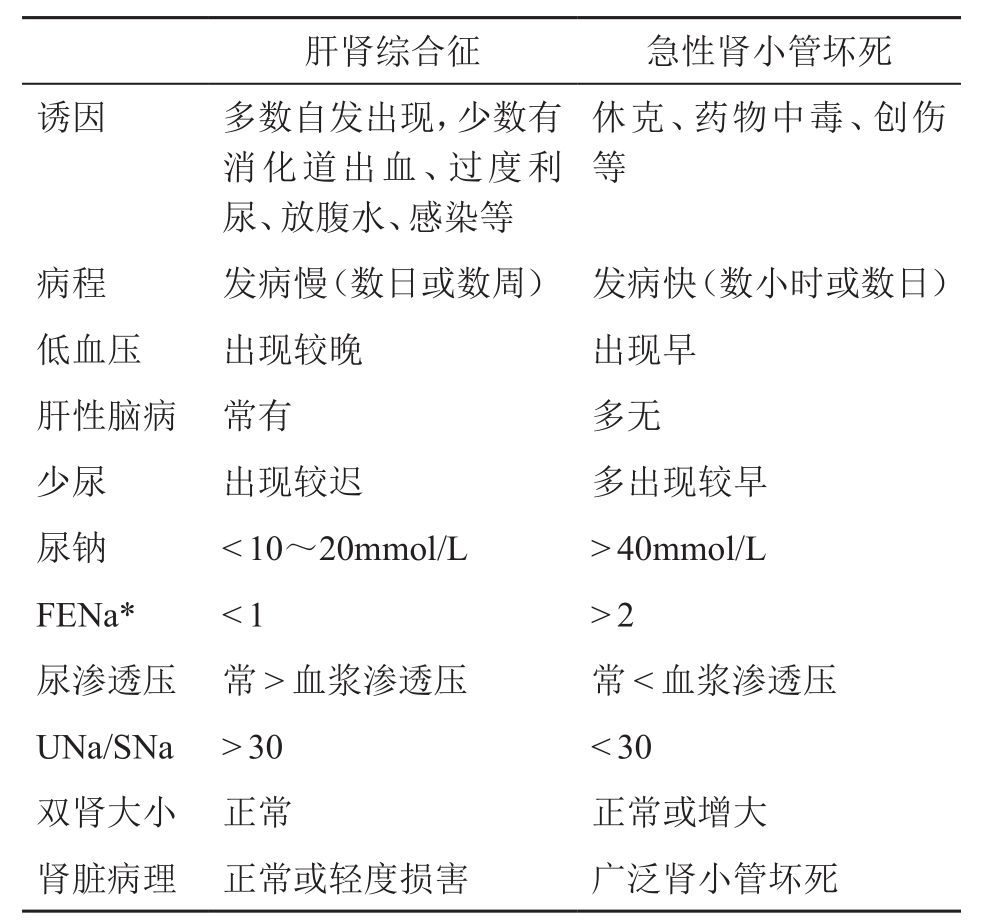
\includegraphics[width=3.32292in,height=3.0625in]{./images/Image00494.jpg}
\end{table}

FENa =滤过钠排泄分数;FENa = UNa•Scr/(SNa•Ucr);UNa =尿钠;SNa
=血清钠;Scr =血清肌酐;Ucr =尿肌酐

\paragraph{全身性疾病}

如脓毒症、钩端螺旋体病、结缔组织病及多囊肝和多囊肾等可同时累及肝肾,有时亦不易鉴别。

\subsection{治疗}

肝功能衰竭患者一旦出现肝肾综合征,多在1~2周内肾功能急剧恶化。患者常死于消化道出血、感染、肝昏迷或多器官功能衰竭,而很少死于肾衰,其临床自发缓解率仅为0~15\%,治疗极其困难。因此在治疗肝病、改善肝功能的同时,应在肾功能损害期即采取措施,改善肾血流量,避免任何原因的有效循环血量的减少,以及任何有损肾功能的因素。病程中一旦出现少尿或无尿,应立即按肝肾综合征采取积极的治疗措施。

\subsubsection{一般措施}

Ⅰ型HRS患者病情凶险且不稳定,需密切监测患者生命体征、液体摄入量、体重、血液生化学指标及尿量。中心静脉压的监测对评价血容量状态十分有意义,尤其对排除由于血容量不足导致的肾功能意义重大。对有稀释性低钠血症的患者,水的摄入应限制在1L/d以下。对有顽固性腹水的患者,治疗性放腹水每次5L,同时输白蛋白6~8g/L,但对Ⅰ型HRS患者,放等量或更多的腹水是否会导致肾功能进一步恶化尚不清楚。

Ⅱ型HRS患者,其危险性较低,且大部分患者的腹水可通过穿刺放液与静脉输注白蛋白得以纠正。

\subsubsection{消除诱因}

有肾毒作用的庆大霉素、卡那霉素等药物及抑制肾内前列腺素合成的非甾体类抗炎药物如水杨酸类、吲哚美辛等,均可使肾功能进一步恶化,应避免使用。任何可以改变血流量的因素如过度利尿、呕吐、腹泻、消化道出血、大量腹腔穿刺放液而没有给相应的扩容治疗,均可导致有效循环血量的急剧减少而诱发HRS,对这些因素均应及时发现予以纠正。

\subsubsection{利尿治疗}

是肝硬化腹水稳定尿量的有效手段。选择利尿药时应注意袢利尿剂与醛固酮拮抗剂要伍用,强或中效利尿剂与弱效利尿剂要伍用。一般以醛固酮拮抗剂为主,辅以作用于升支粗段皮质部的中效利尿剂噻嗪类,后者应以间歇性用药为宜。作用于升支粗段的髓质和皮质部的强利尿剂类常在上述药物无效时应用,不宜作为肝硬化腹水利尿治疗的首选药物。螺内酯常由小剂量开始,每日120~180mg,若5天后不出现疗效,剂量可增至400mg/d。肝硬化腹水患者在一般利尿失效或尿量明显减少,有发展成HRS可能时可用呋塞米。为迅速纠正少尿,呋塞米最大剂量可达160mg/d,如大剂量利尿剂治疗无效,不应继续增加利尿剂剂量,可通过联合用药途径而达到利尿效果。笔者应用呋塞米40~200mg/d联合多巴胺20~80mg腹腔内注射治疗顽固性腹水,有显著疗效。利尿过程中应注意血容量的减少及电解质的紊乱,尤其要注意低钾血症或高血钾。

\subsubsection{血管活性药物的应用}

是近年来HRS治疗研究的进展。其机制是应用扩血管药物起到扩张肾血管、增加肾血流量及肾小球滤过率作用。但临床应用结果尚不完全一致。

\paragraph{血管扩张剂}

多巴胺(dopamine,DA)为选择性肾血管扩张药物。非升压剂量{[}2.0~3.5μg/(kg•min){]}的DA静脉注射可直接刺激肾小球DA受体,改善肾血流量及滤过功能,增加尿钠排泄。多巴酚丁胺为β受体兴奋剂,也有增加肾血流量及尿量作用。多巴胺联合多巴酚丁胺静脉滴注能有效地改善全身循环及维持有效循环血量,比单用多巴胺的肾功能改善作用更佳。前列腺素类如PGE\textsubscript{2}
(米索前列醇)有改善血流,促进钠水排泄及肌酐清除的作用。其机制可能与扩张肾血管、对抗循环中缩血管物质及抵消不正常的肝细胞释放的某些未知激素物质有关。

\paragraph{血管收缩剂}

内脏血管的扩张是HRS的首发因素,因此血管收缩剂合并扩容治疗可有效纠正肾功能衰竭。目前用于HRS的血管收缩剂包括血管加压素类似物(如特利加压素)、生长抑素类似物(如奥曲肽)以及α-肾上腺素能激动剂(米多君和去甲肾上腺素)。血管收缩剂对Ⅰ型HRS的应用指南:①治疗目的:降低血清肌酐水平使其小于133μmol/L。②推荐药物及剂量:特利加压素(terlipressin):静脉滴注,每4小时0.5mg,可逐步提高剂量(每2~3天)至每4小时1mg,若血清肌酐水平没有降低,可增至每4小时2mg。奥曲肽(octreotide):该药具有降低血管阻力、增加肾皮质血流量的作用,因而可使肾小球滤过率增加。开始剂量一般为0.1μg/min,必要时可增加剂量,据报道对血压偏低的患者疗效较好。米多君(midodrine,甲氧氨福林):口服,2.5~7.5mg/次,每天3次,可增至12.5mg/次,同时奥曲肽皮下注射,100μg/次,每天3次,可增至200μg/次。去甲肾上腺素:0.5~3mg/h持续静脉滴注。③同时静脉应用白蛋白,第1天1g/kg,继以20~50g/d(若血白蛋白>
45g/L或出现肺水肿时停用),可起到扩充血容量的作用。④血管收缩剂可能导致缺血,应当避免患者发生心脏疾病、外周血管疾病以及脑血管病。⑤疗程:1~2周。

\subsubsection{扩容治疗}

有效的扩容能纠正低血容量,增加肾血流量及肾小球滤过率,对改善肾功能有明显作用。除常用的扩容剂外,浓缩腹水回输治疗,既能补充蛋白,提高血浆胶体渗透压,又是有效的扩容治疗方法,但应避免发生感染及DIC等。扩容治疗应适当,以防发生心衰、肺水肿及食管静脉曲张破裂出血等并发症,一般依据临床状况(尿量、血压、血肌酐等)及中心静脉压(CVP)作为检测指标,在30~60分钟内静滴500~1000ml,尿量达30ml/h以上或超过补液前12小时尿量则应继续补液。有条件可在监测中心静脉压的情况下进行,补液至CVP≥8~10cmH\textsubscript{2}
O即可。

\subsubsection{大容量腹腔穿刺放液(LVP)}

这种传统的方法近年来已受到重视。大容量腹腔穿刺放液能快速消除腹水,改善病情,且副作用小,但必须与扩容治疗联合进行,否则会致有效血容量进一步减少,诱发肝性脑病或肾功能恶化。实施大容量腹腔穿刺治疗,一般每次放腹水可达5~6L或全部放完,但必须同时静脉滴注白蛋白40g或6~8g/L。有报道用右旋糖酐70(每升腹水补100ml)替代白蛋白作扩容治疗,疗效相似,且费用可大大减少。

\subsubsection{经颈静脉肝内门体分流术(TIPS)}

TIPS对包括HRS在内的肾功能具有积极的作用。它可以迅速提高尿钠外排、尿量、改善血清肌酐浓度。此外,TIPS术后,血浆肾素活性、醛固酮、去甲肾上腺素迅速提高,可能在HRS血容量不足方面发挥积极作用。TIPS的积极作用被肝性脑病越来越频繁的发生和严重的发作所阻碍,但其阻碍作用可通过筛选患者和降低旁路直径而降低。对Ⅰ型HRS患者中Child-Push评分大于12者,TIPS不适用,因为它可加重肝功能衰竭和肝性脑病。对Ⅱ型HRS患者可改善肾功能并减少腹水。TIPS对酒精性及血吸虫性肝硬化合并肾功能衰竭者疗效明显为佳。但是大规模研究表明对肝性脑病、肝功能衰竭以及重症凝血机制障碍者TIPS后并发症较多。国外将其作为肝移植前的过渡。

\subsubsection{血液净化治疗}

血液净化治疗方式包括血液透析、连续性肾脏替代治疗(CRRT,包括CAVH、CAVHD、CVVHD)、治疗性血浆置换、血液灌流等可清除多种对肝肾功能有害的物质,如氨、假性神经递质、细胞因子(IL-6、IL-1、TNF)、中分子物质、内毒素、胆红素、胆酸、硫醇等。通过净化治疗,可以改善肾功能,保证血容量平衡,纠正氮质血症和酸中毒,预防急性肺水肿等致命性并发症,且为输注碳酸氢钠、营养和血制品等提供条件。分子吸附再循环系统用于治疗Child-C级肝硬化患者以及Ⅰ型HRS患者效果显著。

\subsubsection{肝移植}

肝移植包括原位肝移植(OLT)及肝肾联合移植(SLKT)。对于肾功能不全接受OLT的患者,目前多考虑肝肾联合移植。但应特别注意的是:SLKT患者可能会发生可逆性肾功能衰竭。有慢性肾病史,肌酐清除率≤30ml/min(采用碘酞酸盐类清除率更好)是考虑SLKT的适当阈值,仅有HRS不应被作为SLKT的理由。但是,目前认为,如果HRS患者进展为透析依赖,或在透析6~8周后(急性肾损伤常规恢复时间)尚未恢复,仍可考虑进行SLKT。肝移植是治疗具有肝移植指征的HRS患者最佳方法,但是对Ⅰ型患者移植率很低,主要是由于生存时间较短以及等待时间较长而在术前死亡。

\subsubsection{中西医药联合治疗}

应用丹参或川芎嗪注射液等配合血管活性药物或利尿剂治疗HRS,有一定疗效,但需要更多的基础及临床研究进一步证实。

总之,对HRS的治疗应按分型进行。对Ⅰ型HRS患者的治疗措施包括应用血管收缩剂及TIPS。Ⅱ型HRS患者,其危险性较低,且大部分患者的腹水可通过穿刺放液与静脉输注白蛋白得以纠正。\hypertarget{text00330.htmlux5cux23CHP11-7-3-4}{}
参 考 文 献

1. SфREN MфLLER. Pathophysiological basis of pharmacotherapy in the
hepatorenal syndrome. Scandinavian Fournal of
Gastroenterology,2005,40:491-500.

2. MσNICA Guevara Pere Ginès. Hepatorenal Syndrome. Dig
Dis,2005,23:47-55.

3. Mackelaite L,Alsauskas ZC,Ranganna K. Renal failure in patients
with cirrhosis. Med Clin North Am,2009,93:855-869.

4. Salerno F,Gerbes A,Ginès P,et al. Diagnosis,prevention and
treatment of hepatorenal syndrome in cirrhosis.
Gut,2007,56(9):1310-1318.

5. Moreau R,Lebrec D. The use of vasoconstrictors in patients with
cirrhosis:type 1 HRS and beyond. Hepatology,2006,43:385-394.

\protect\hypertarget{text00331.html}{}{}

